 %%
%% This is file `elsarticle-template-num.tex',
%% generated with the docstrip utility.
%%
%% The original source files were:
%%
%% elsarticle.dtx  (with options: `numtemplate')
%% 
%% Copyright 2007, 2008 Elsevier Ltd.
%% 
%% This file is part of the 'Elsarticle Bundle'.
%% -------------------------------------------
%% 
%% It may be distributed under the conditions of the LaTeX Project Public
%% License, either version 1.2 of this license or (at your option) any
%% later version.  The latest version of this license is in
%%    http://www.latex-project.org/lppl.txt
%% and version 1.2 or later is part of all distributions of LaTeX
%% version 1999/12/01 or later.
%% 
%% The list of all files belonging to the 'Elsarticle Bundle' is
%% given in the file `manifest.txt'.
%% 

%% Template article for Elsevier's document class `elsarticle'
%% with numbered style bibliographic references
%% SP 2008/03/01

%\documentclass[preprint,12pt]{elsarticle}
\documentclass[review,10pt]{elsarticle}
%\documentclass[final,3p,times]{elsarticle} 

%% Use the option review to obtain double line spacing
%% \documentclass[authoryear,preprint,review,12pt]{elsarticle}

%% Use the options 1p,twocolumn; 3p; 3p,twocolumn; 5p; or 5p,twocolumn
%% for a journal layout:
%% \documentclass[final,1p,times]{elsarticle}
%% \documentclass[final,1p,times,twocolumn]{elsarticle}
%% \documentclass[final,3p,times]{elsarticle}
%% \documentclass[final,3p,times,twocolumn]{elsarticle}
%% \documentclass[final,5p,times]{elsarticle}
%% \documentclass[final,5p,times,twocolumn]{elsarticle}

%% if you use PostScript figures in your article
%% use the graphics package for simple commands
\usepackage{float}
\usepackage{color}
\usepackage{caption}
\usepackage{subcaption}
\usepackage{appendix}
%% or use the graphicx package for more complicated commands
\usepackage{graphicx}
%% or use the epsfig package if you prefer to use the old commands
%% \usepackage{epsfig}

%% The amssymb package provides various useful mathematical symbols 
%% The amsthm package provides extended theorem environments
\usepackage{amssymb}
\usepackage{amsmath}
% more math
\usepackage{amsfonts}
\usepackage{amstext}
\usepackage{amsbsy}
\usepackage{mathbbol} 
%% The lineno packages adds line numbers. Start line numbering with
%% \begin{linenumbers}, end it with \end{linenumbers}. Or switch it on
%% for the whole article with \linenumbers.
\usepackage{lineno}
\usepackage{cancel}
\usepackage{setspace}
\doublespacing

\journal{Computers \& Fluids}
%%%%%%%%%%%%%%%%%%%%%%%%%%%%%%%%%%%%%%%%%%%%%%%%%%%%%%%%%%%%%%%%%%%%
% operators
\renewcommand{\div}{\vec{\nabla}\! \cdot \!}
\newcommand{\grad}{\vec{\nabla}}
\newcommand{\divv}[1]{\vec{\nabla}^{#1}\! \cdot \!}
\newcommand{\gradd}[1]{\vec{\nabla}^{#1}}
% latex shortcuts
\newcommand{\bea}{\begin{eqnarray}}
\newcommand{\eea}{\end{eqnarray}}
\newcommand{\be}{\begin{equation}}
\newcommand{\ee}{\end{equation}}
\newcommand{\bal}{\begin{align}}
\newcommand{\eali}{\end{align}}
\newcommand{\bi}{\begin{itemize}}
\newcommand{\ei}{\end{itemize}}
\newcommand{\ben}{\begin{enumerate}}
\newcommand{\een}{\end{enumerate}}
% DGFEM commands
\newcommand{\jmp}[1]{[\![#1]\!]}                     % jump
\newcommand{\mvl}[1]{\{\!\!\{#1\}\!\!\}}             % mean value
\newcommand{\keff}{\ensuremath{k_{\textit{eff}}}\xspace}
% shortcut for domain notation
\newcommand{\D}{\mathcal{D}}
% vector shortcuts
\newcommand{\vo}{\vec{\Omega}}
\newcommand{\vr}{\vec{r}}
\newcommand{\vn}{\vec{n}}
\newcommand{\vnk}{\vec{\mathbf{n}}}
\newcommand{\vj}{\vec{J}}
\newcommand{\eig}[1]{\| #1 \|_2}

\newcommand{\EI}{\mathcal{E}_h^i}
\newcommand{\ED}{\mathcal{E}_h^{\partial \D^d}}
\newcommand{\EN}{\mathcal{E}_h^{\partial \D^n}}
\newcommand{\ER}{\mathcal{E}_h^{\partial \D^r}}
\newcommand{\reg}{\textit{reg}}

\newcommand{\norm}{\textrm{norm}}
\renewcommand{\Re}{\textrm{Re}}
\newcommand{\Pe}{\textrm{P\'e}}
\renewcommand{\Pr}{\textrm{Pr}}

\newcommand{\resi}{R_\text{ent}}
%\newcommand{\resinew}{\tilde{D}_e}
\newcommand{\resinew}{\widetilde{R}_\text{ent}}
\newcommand{\matder}[1]{\frac{\textrm{D} #1}{\textrm{D} t}}


% extra space
\newcommand{\qq}{\quad\quad}
% common reference commands
\newcommand{\eqt}[1]{Eq.~(\ref{#1})}                     % equation
\newcommand{\fig}[1]{Fig.~\ref{#1}}                      % figure
\newcommand{\tbl}[1]{Table~\ref{#1}}                     % table
\newcommand{\sct}[1]{Section~\ref{#1}}                   % section
\newcommand{\app}[1]{Appendix~\ref{#1}}                   % appendix
\newcommand{\rmk}[1]{Remark~\ref{#1}}                   % remark

\newcommand\br{\mathbf{r}}
%\newcommand{\tf}{\varphi}
\newcommand{\tf}{b}

\newcommand{\tcr}[1]{\textcolor{red}{#1}}
\newcommand{\tcb}[1]{\textcolor{blue}{#1}}
\newcommand{\mt}[1]{\marginpar{ {\tiny \tcr{#1} }}}

\newtheorem{remark}{Remark}

\bibliographystyle{elsarticle-num}
%%%%%%%%%%%%%%%%%%%%%%%%%%%%%%%%%%%%%%%%%%%%%%%%%%%%%%%%%%%%%%%%%%%%%
%
%   BEGIN DOCUMENT
%
%%%%%%%%%%%%%%%%%%%%%%%%%%%%%%%%%%%%%%%%%%%%%%%%%%%%%%%%%%%%%%%%%%%%%
\begin{document}

%%%%%%%%%%%%%%%%%%%%%%%%%%%%%%%%%%%%%%%%%%%%%%%%%%%%%%%%%%%%%%%%%%%%
\begin{frontmatter}

%% Title, authors and addresses

%% use the tnoteref command within \title for footnotes;
%% use the tnotetext command for theassociated footnote;
%% use the fnref command within \author or \address for footnotes;
%% use the fntext command for theassociated footnote;
%% use the corref command within \author for corresponding author footnotes;
%% use the cortext command for theassociated footnote;
%% use the ead command for the email address,
%% and the form \ead[url] for the home page:
%\title{Title\tnoteref{label1}}
%% \tnotetext[label1]{}
%% \author{Name\corref{cor1}\fnref{label2}}
%% \ead{email address}
%% \ead[url]{home page}
%% \fntext[label2]{}
%% \cortext[cor1]{}
%% \address{Address\fnref{label3}}
%% \fntext[label3]{}
%-------------------------
%-------------------------
%\title{Extension of the entropy viscosity method to the low Mach regime for the multi-dimensional Euler equations\\
\title{Entropy-based viscous regularization for the multi-dimensional Euler equations in low-Mach and transonic flows}
%-------------------------
%-------------------------
\author{Marc O. Delchini\fnref{label1}}
\ead{delchmo@tamu.edu}

\author{Jean C. Ragusa\corref{cor1}\fnref{label1}}
\ead{jean.ragusa@tamu.edu}

\author{Ray A. Berry\fnref{label2}}
\ead{ray.berry@inl.gov}

\address[label1]{Department of Nuclear Engineering, Texas A\&M University, College Station, TX 77843, USA \fnref{label1}}

\address[label2]{Idaho National Laboratory, Idaho Falls, ID 83415, USA \fnref{label2}}

\cortext[cor1]{Corresponding author}
%-------------------------
%-------------------------
%-------------------------
\begin{abstract}
%We show that the current version of the entropy viscosity method, a viscous regularization technique for hyperbolic 
%conservation laws, is not well-suited to low-Mach flows. 
We present a new version of the entropy viscosity method, a viscous regularization technique for hyperbolic 
conservation laws, that is well-suited to low-Mach flows. 
By means of a low-Mach asymptotic study, new expressions for the entropy viscosity coefficients are derived.
These definitions are valid for a wide range of Mach numbers, from subsonic flows (with very low Mach  numbers) to 
supersonic flows, and no longer depend on an analytical expression for the entropy function.
In addition, the entropy viscosity method is extended to Euler equations with variable area for nozzle flow problems.
%
%and our numerical results confirm that the new expressions are valid for a wide range of Mach numbers, from subsonic flows (with very low Mach  numbers) to supersonic flows. 
%The new expressions for the entropy viscosity coefficients, obtained by means of an low-Mach asymptotic study,
%  We show that, in the existing method, the definition of the viscosity coefficients is not adapted to low-Mach flows 
%and we provide a robust alternate definition valid for any Mach number value by means of an asymptotic study. 
%The entropy viscosity method is also extended to Euler equations with variable area for nozzle flow problems.
 %In addition, the entropy minimum principle is used to derive the viscous regularization terms for Euler equations with 
%variable area for nozzle flow problems. 
The effectiveness of the method is demonstrated using various 1-D and 2-D benchmark tests: flow in a converging-diverging 
nozzle; Leblanc shock tube; slow moving shock; strong shock for liquid phase; low-Mach flows around a 
cylinder and over a circular hump; and supersonic flow in a compression corner. 
Convergence studies are performed for both smooth solutions and solutions with shocks present. 
%The ideal gas and stiffened gas equations of state are employed.
\end{abstract}
%-------------------------
%-------------------------
\begin{keyword}
  entropy viscosity method \sep artificial  viscosity \sep low-Mach regime \sep shock capturing \sep Euler equations with variable area.
\end{keyword}
%-------------------------
\end{frontmatter}
%%%%%%%%%%%%%%%%%%%%%%%%%%%%%%%%%%%%%%%%%%%%%%%%%%%%%%%%%%%%%%%%%%%%
\linenumbers
%%%%%%%%%%%%%%%%%%%%%%%%%%%%%%%%%%%%%%%%%%%%%%%%%%%%%%%%%%%%%%%%%%%%%%%%%%%%%%%%%%%%%%%%%%%%%%%%%%%%
%%%%%%%%%%%%%%%%%%%%%%%%%%%%%%%%%%%%%%%%%%%%%%%%%%%%%%%%%%%%%%%%%%%%%%%%%%%%%%%%%%%%%%%%%%%%%%%%%%%%
\section{Introduction} \label{sec:intro}
%%%%%%%%%%%%%%%%%%%%%%%%%%%%%%%%%%%%%%%%%%%%%%%%%%%%%%%%%%%%%%%%%%%%%%%%%%%%%%%%%%%%%%%%%%%%%%%%%%%%
%%%%%%%%%%%%%%%%%%%%%%%%%%%%%%%%%%%%%%%%%%%%%%%%%%%%%%%%%%%%%%%%%%%%%%%%%%%%%%%%%%%%%%%%%%%%%%%%%%%%
%\tcr{I need to continue working on the Introduction} \tcb{what is it you want to change?}

%\tcr{ not finished yet\\
%Items to mention:
%\begin{itemize}
%\item low Mach solution techniques using compressible equations. need to recover the incompressible limit. 
%\item entropy viscosity method, not yet assessed for low Mach and transonic flows
%\item low Mach also challenging when solved using compressible equations: if explicit, time step $\rightarrow 0$. We use MOOSE and implicit time stepping
%\item some flow problems have both low Mach and supersonic regions
%\item OTHERS ???
%\item 
%\end{itemize}
%}
%\tcr{I think we should focus the introduction more}
%
%Incompressible flows are a particular case of compressible ones and therefore in principle, a
%compressible flow solver should be able to compute these flows. Unfortunately, there are experimental
%evidences showing that on a fixed mesh, the solutions of the compressible flow discretized
%equations are not an accurate approximation of the solutions of the incompressible model (e.g. see
%[29]). A first analysis of this problem appeared in [23] and this question has drawn a considerable
%attention [1–3,7,9,26,28,30] in the recent past. Several works have tried to explain the reasons of
%this difficulty and to construct numerical schemes valid for all Mach numbers. Some of these
%works extend to the compressible regime the numerical methods used for the computation of
%incompressible flows. Examples of these type of methods are for instance [1] or [30]. Another
%approaches rely on some modifications of high order shock capturing techniques. These approaches
%are for instance described in [2,7,22] for Roe discretization, in [3] for the HLLE scheme
%and in [28] for Flux schemes. Their principal ingredient is the use of preconditioning techniques
%originally developed for steady state computations [4,21,23] that are here selectively applied only
%to the upwind artificial viscosity.
%
%
%The efficient simulation of low Mach number flows is a subject of ongoing discussion in the
%CFD community. While the flow is expected to be incompressible, in a lot of applications
%the Mach number or the compressibility properties vary strongly in time or space. This is
%for example the case in nozzle  flow, chemically reacting flows or laminar combustion. It is
%well known that purely compressible flow solvers which were developed for transonic 
%flow produce wrong results at low Mach numbers. On the other hand, standard incompressible 
%flow solvers cannot deal with strong temperature or strong density gradients. This sets a
%demand for codes that can deal with flows at all Mach numbers.
%
%It is well known that it is difficult to solve the compressible equations for low Mach numbers.
%For an explicit scheme this is easily seen by looking at the time steps. For stability the time
%step must be chosen inversely proportional to the largest eigenvalue of the system which is
%approximately the speed of sound, c, for slow flows. However, other waves are convected at the
%fluid speed, u, which is much slower. Hence, these waves don’t change very much over a time
%step. Thus, thousands of time steps are required to reach a steady state. Should one try a
%multigrid acceleration one finds that the same disparity in wave speeds slows down the
%multigrid acceleration. With an implicit method an AD1 factorization is usually used so that
%one can easily invert the implicit factors. The use of AD1 introduces factorization errors which
%again slow down the convergence rate when there are wave speeds of very different magnitudes
%For small Mach numbers it can be shown [28,31] that the incompressible equations approximate
%the compressible equations. Hence, one needs to justify the use of the compressible
%equations for low Mach flows. We present several reasons why one would still use the
%compressible equations even though the Mach number of the flow is small.
%l There are many sophisticated compressible codes available that could be used for such
%problems especially in complicated geometries.
%l For low speed aerodynamic problems at a high angle of attack most of the flow consists of
%a low Mach number flow. However, there are localized regions containing shocks.
%l In many problems thermal effects are important and the energy equation is coupled to the
%other equations.
%
%The incompressible limit of a compressible flow is rather subtle due to the fact that the propagation rate of
%the pressure waves becomes infinite and the equations change their type. Within this limit the pressure splits up
%into a thermodynamic pressure term and a hydrodynamic pressure term. If the limit solution has constant
%temperature and density and if the boundary values satisfy the incompressibility constraint, then the
%thermodynamic pressure becomes the background pressure being constant in space and time. The hydrodynamic
%pressure appears in the incompressible equations as a sort of a Lagrangian multiplier with no connection
%to the equation of state. The asymptotic analysis of Klainerman and Majda in [9,10] gives insight into this
%limit behavior. They gave a mathematically rigorous derivation in the isentropic case. The asymptotic analysis
%was formally extended by Klein to the non-isentropic case and to multiple space scales in [11] in which he also
%gave an overview about other asymptotic considerations in this low Mach number regime. A detailed discussion
%of the incompressible limit is also given in the book of Wesseling [20].
%Numerical methods for the compressible equations may have difficulties with the zero Mach number limit
%because in the limit the speed of sound waves becomes infinite compared to the flow speed and thus leads to an
%elliptic coupling of pressure and velocity. Hence, all explicit numerical schemes become quite inefficient in the
%low Mach number regime due to their stability restriction (CFL condition). The other difficulty is that the
%pressure in the compressible equations converges to the thermodynamic pressure, which becomes the constant
%background pressure in the incompressible limit. This is the way how the equation of state for compressible
%flow is automatically satisfied and does not appear in the incompressible equations. For the compressible
%equations Bijl and Wesseling [2] introduced a splitting of the pressure into a thermodynamic and a hydrodynamic
%pressure term. Then they proposed an implicit numerical method that remains stable without reference
%to the sound velocity and which approximates the incompressible equations for Mach number zero. The constant
%thermodynamic pressure satisfies the equation of state and the hydrodynamic pressure serves as a
%Lagrangian multiplier to get the divergence-free property of the velocity. A formulation in conservative variables
%was later given in [18,20]. Similar to this approach Klein and Munz [12] and Munz et al. [13] proposed
%%the multiple pressure variable (MPV) method based on the asymptotic results of Klein [11].
%
%\tcr{above are good snippets from some papers.}

%While the flow is expected to be incompressible, in a lot of applications
%the Mach number or the compressibility properties vary strongly in time or space. This is
%for example the case in nozzle  flow, chemically reacting flows or laminar combustion. It is
%well known that purely compressible flow solvers which were developed for transonic 
%flow produce wrong results at low Mach numbers. On the other hand, standard incompressible 
%flow solvers cannot deal with strong temperature or strong density gradients. This sets a
%demand for codes that can deal with flows at all Mach numbers.

Solving accurately compressible fluid equations in the low-Mach limit is an ongoing topic of research. 
In many engineering applications, compressibility effects require the solution of the compressible fluid equations
in nearly incompressible regimes and/or for low-Mach flow problems. For example, such flows are encountered 
in aerodynamics in the study of airships. In the nuclear industry, flows are nearly in the incompressible regime but 
compressible effects cannot be neglected because of the intense heat source, and because of some postulated accident scenarios, 
and thus need to be accurately resolved. Hence, there is a strong interest to develop computational methods 
that can solve both compressible and incompressible flow problems.  

When solving Euler equations for a wide range of Mach numbers, multiple questions must be addressed: stability, 
accuracy and solution convergence in the low-Mach regime. Because of the hyperbolic nature of the equations, 
shocks can form during transonic and supersonic flows and require the use of adequate numerical techniques to stabilize solution
and correctly resolve the discontinuities. A wide range of stabilization methods are available in the literature: approximate Riemann solvers \cite{Toro}, flux-limiter techniques 
\cite{FluxLimiter, FluxLimiter2}, pressure-based viscosity methods \cite{PBV_book}, Lapidus method \cite{Lapidus_paper, LMP, Lapidus_book}, 
and the entropy-viscosity method \cite{jlg1, jlg2}, among others. These numerical methods are usually developed using simple equations 
of state and tested for transonic and supersonic flows where the disparity between the acoustic wave speed and the fluid speed is not 
excessively large and thus the Mach number is of order one. This approach, however, leads to a well-known accuracy problem in the low-Mach regime 
where the fluid velocity is smaller that the speed of sound by multiple orders of magnitude. The numerical dissipative terms become 
ill-scaled in the low-Mach regime and lead to the wrong numerical solution by changing the nature of the equations solved. This 
behavior is well documented in the literature \cite{LowMach1, LowMach2, LowMach3}.
% and often treated by performing a low-Mach  asymptotic study of Euler equations. 
In \cite{LowMach1}, a low-Mach asymptotic study has demonstrated convergence of the 
compressible Euler equations to the incompressible ones. 
Many well-known stabilization techniques, for instance, the Roe scheme and the SUPG technique,
do not yield the correct solution in the low-Mach regime and suitable modifications have been proposed (see \cite{Roe} for the Roe scheme and \cite{LowMach3} for the SUPG method)
to ensure the convergence to the correct solution while preserving the original shock stabilization 
properties of these schemes. 
%
%Using an asymptotic approach, the effect of the dissipative 
%terms 
%%
%\tcr{not clear for a reader, what dissipative are you talking about? you just said Euler equation and you have not made the link in the above text between stabilization techniques and dissipative terms. I think a reader who only does DG would not understand what you are trying to say}
%%
%in the low-Mach regime can be understood and, when needed, a fix is developed in order to ensure the convergence of the 
%equations to the correct physical solution. This approach was used as a ``fixing'' method for multiple well-known stabilization 
%methods, for instance, the Roe scheme (\cite{Roe}) and the SUPG technique \cite{LowMach3}, while preserving the original stabilization 
%properties for shocks. 
Additionally, the time step size may be severely restricted when solving compressible fluid equations with an explicit time discretization 
because of the large disparity between the fluid velocity and the speed of sound. 
To avoid an excessive number of explicit time steps, time preconditioners have been proposed and proved efficient \cite{LowMach2};
however, because they modify the time derivatives in the governing equations, such acceleration techniques can only be used to obtain
steady-state solutions for low-Mach flows using explicit schemes.
%for stability purpose, the time step must be chosen inversely proportional to the largest eigenvalue of the 
%system which is approximately the speed of sound, $c$, for slow flows. However, other waves are convected at the fluid speed, which may 
%be significantly smaller than $c$. Hence, these waves do not change very much over a time step. Thus, thousands of time steps are required 
%to reach a steady state. Acceleration techniques were developed and proved efficient \cite{LowMach2} but require the modification of the 
%temporal derivatives of the equation and, thus, can only be used for steady-state flows. 
To avoid modifying the time derivatives, 
the temporal implicit capabilities of the MOOSE multiphysics framework \cite{MOOSE} are used. With such a choice, low-Mach steady-state solutions 
can be obtained effectively while preserving the accuracy of the transient solution; however, it requires the use of nonlinear solvers.

In this paper, we employ the entropy viscosity method as a numerical stabilization for the inviscid Euler equation and assess its performance 
in the low-Mach regime. 
The entropy viscosity method is a viscous regularization technique introduced by Guermond et al. to solve hyperbolic systems of equations
and has successfully been applied to multi-dimensional supersonic flows with various spatial discretization schemes \cite{jlg}. 
It is fairly straightforward to implement, can be used with unstructured grids, and has dissipative terms that are consistent with the 
entropy minimum principle. However, it has not been evaluated in the low-Mach regime.

This paper is organized as follows: in \sct{sec:entro_visc} the current definition of the entropy viscosity method is recalled and 
its ill-scaled nature in the low-Mach regime is discussed. 
In \sct{sec:extension}, a new formulation of the viscosity residual is derived. This formulation no longer requires an analytical expression 
for the entropy function. A low-Mach asymptotic study is carried out to adapt the definition of the entropy viscosity coefficients 
in the incompressible limit while ensuring that the viscosity coefficients scale appropriately for all flow speeds (from low-Mach to supersonic).
%
In  \sct{sec:var_area_diss_terms}, we extend the entropy viscosity method to Euler equations with variable area in order to model nozzle flows: 
the viscous dissipative terms are adapted so that the entropy minimum principle remains satisfied.
Spatial and temporal discretizations and solution tehcniques are presented in \sct{sec:solution_tech}.
 1-D and 2-D numerical results 
are provided in \sct{sec:results} for a wide range of Mach numbers: liquid and gas nozzle flow problems, 
low-Mach flows over a cylinder and a circular bump (with Mach numbers as low as $10^{-7}$), and supersonic flows 
in a compression corner \cite{CompressionCorner}. 
Convergence studies are performed in 1-D in order to demonstrate the accuracy of the solution technique. 

% keep this as a comment for now
%\tcr{I wouldn't recall this here. Let me think about that.}\\
%For purpose of clarity, the multi-D Euler equations with variable area are recalled in \eqt{eq:euler_eq} and the corresponding variables are defined:
%%
%\begin{equation}
%\label{eq:euler_eq}
%\left\{ 
%\begin{array}{lll}
%\partial_t \left( \rho A\right) + \div \left( \rho \vec{u} A\right) = 0\\
%\partial_t \left( \rho \vec{u} A\right) + \div \left[ \left( \rho \vec{u} \otimes \vec{u} + P \mathbf{I} \right) A \right] = P \grad A\\
%\partial_t \left( \rho E A\right) + \div \left[ \vec{u} \left( \rho E + P \right) A\right] = 0 \\
%P = P\left( \rho, e \right)
%\end{array}
%\right.
%\end{equation}

%%%%%%%%%%%%%%%%%%%%%%%%%%%%%%%%%%%%%%%%%%%%%%%%%%%%%%%%%%%%%%%%%%%%%%%%%%%%%%%%%%%%%%%%%%%%%%%%%%%%
%%%%%%%%%%%%%%%%%%%%%%%%%%%%%%%%%%%%%%%%%%%%%%%%%%%%%%%%%%%%%%%%%%%%%%%%%%%%%%%%%%%%%%%%%%%%%%%%%%%%
\section{The Entropy Viscosity Method} \label{sec:entro_visc}
%%%%%%%%%%%%%%%%%%%%%%%%%%%%%%%%%%%%%%%%%%%%%%%%%%%%%%%%%%%%%%%%%%%%%%%%%%%%%%%%%%%%%%%%%%%%%%%%%%%%
%%%%%%%%%%%%%%%%%%%%%%%%%%%%%%%%%%%%%%%%%%%%%%%%%%%%%%%%%%%%%%%%%%%%%%%%%%%%%%%%%%%%%%%%%%%%%%%%%%%%

%===================================================================================================
\subsection{Background} \label{sec:background}
%===================================================================================================

Euler equations in conservative form are given by
\begin{subequations}
\label{eq:euler_eq}
%
\begin{equation}
\partial_t \rho  + \div \left( \rho \vec{u} \right) = 0
\end{equation}
%
\begin{equation}
\partial_t \left( \rho \vec{u} \right) + \div \left( \rho \vec{u} \otimes \vec{u} + P \mathbb{I} \right) = 0 
\end{equation}
%
\begin{equation}
\partial_t \left( \rho E \right) + \div \left[ \vec{u} \left( \rho E + P \right) \right] = 0
\end{equation}
\end{subequations}
%
where $\rho$, $\rho \vec{u}$ and $E$ are the density, the momentum and the total specific energy, 
respectively, and will be referred to as the conservative variables. $\vec{u}$ is the fluid velocity and 
its specific internal energy is denoted by $e=E-\tfrac{u^2}{2}$. An equation of state, dependent upon 
$\rho$ and $e$, is used to compute the pressure $P$. The tensor product $\vec{a} \otimes \vec{b}$ is 
such that $(\vec{a} \otimes \vec{b})_{i,j} = a_i b_j$. The identity tensor is denoted by $\mathbb{I}$.

Next, the entropy viscosity method \cite{jlg1, jlg2, jlg3, valentin} applied to \eqt{eq:euler_eq} is 
recalled. The method consists of adding dissipative terms with a viscosity coefficient modulated by 
the entropy production; this allows for a high-order accuracy when the solution is smooth (provided 
that the spatial and temporal discretizations also are high order). 
The derivation of the viscous regularization (or dissipative terms) is carried out to be consistent 
with the entropy minimum principle; details and proofs of the derivation can be found in \cite{jlg}. 
The viscous regularization thus obtained is valid for any equation of state as long as the physical 
entropy function $s$ is concave (or $-s$ is a convex function) with respect to the internal energy 
$e$ and the specific volume $1/\rho$.  The Euler equations with viscous regularization become %are given in \eqt{eq:euler_visc}:
%
\begin{subequations}
\label{eq:euler_visc}
%
\begin{equation}
\partial_t \rho  + \div \left( \rho \vec{u} \right) = \div \left( \kappa \grad \rho \right) 
\end{equation}
%
\begin{equation}
\partial_t \left( \rho \vec{u} \right) + \div \left( \rho \vec{u} \otimes \vec{u} + P \mathbb{I} \right) = \div \left( \mu \rho \grad^s \vec{u}  + \kappa \vec{u} \otimes \grad \rho \right)  
\end{equation}
%
\begin{equation}
\partial_t \left( \rho E \right) + \div \left[ \vec{u} \left( \rho E + P \right) \right] = \div \left( \kappa \grad \left( \rho e \right) + \frac{1}{2}|| \vec{u} ||^2 \kappa \grad \rho +  \rho \mu \vec{u} \grad \vec{u}  \right) 
\end{equation}
\end{subequations}
%
where $\kappa$ and $\mu$ are positive viscosity coefficients (in units of length$^2$/time). $\grad^s \vec{u}$ denotes the symmetric 
gradient operator and  guarantees the method to be rotationally invariant \cite{jlg}. The viscosity 
coefficients are key ingredients in the viscous regularization of \eqt{eq:euler_visc}.  
Other stabilization approaches have been proposed in the literature, for instance, the Lapidus method 
\cite{Lapidus_book, Lapidus_paper} or pressure-based viscosity methods \cite{PBV_book}. Here, we follow 
the work of Guermond et al. and define the viscosity coefficients, $\kappa$ and $\mu$, based on the 
local entropy production. These coefficients are numerically evaluated using the local entropy 
residual $\resi(\vec{r},t)$ defined in \eqt{eq:ent_residual}; $\resi(\vec{r},t)$ is known to be 
peaked in shocks and vanishingly small elsewhere \cite{Toro}. 
%
\begin{equation}
\label{eq:ent_residual}
\resi(\vec{r}, t) := \partial_t s + \vec{u} \cdot \grad s
\end{equation}
%
In the current version of the method, the ratio of $\kappa$ to $\mu$ is defined through a numerical 
Prandlt number, $\Pr = \kappa / \mu$.  $\Pr$ is a user-defined parameter and is usually taken in the 
range $[ 0.001; 1 ]$. Since the entropy residual $\resi(\vec{r},t)$ may be extremely large in shocks, 
the definition of the viscosity coefficients also includes a first-order viscosity coefficient that 
serves as an upper bound for the entropy-based viscosity coefficients. The first-order viscosity 
coefficients, denoted by $\mu_{\max}$ and $\kappa_{\max}$, are chosen so that the numerical scheme 
becomes equivalent to an upwind scheme when the first-order coefficients are employed. The upwind 
scheme is known to be over-dissipative but guarantees monotonicity \cite{Toro}. In practice, the 
viscosity coefficients only saturate to the first-order viscosity coefficients in shocks and are 
much smaller elsewhere, hence avoiding the over-dissipation of the upwind method.  The first-order 
viscosity coefficients $\mu_{\max}$ and $\kappa_{\max}$ are equal and set proportional to the 
largest local eigenvalue $|| \vec{u} || + c $:
%
\begin{equation}
\label{eq:fo}
\mu_{\max}(\vec{r}, t) = \kappa_{\max}(\vec{r}, t) = \frac{h}{2} \left( || \vec{u}(\vec{t,r}) || + c(\vec{t,r}) \right),
\end{equation}
%
where $h$ denotes the local grid size (for higher than linear finite element representations, $h$ is defined 
as the ratio of the grid size to the polynomial order of the test functions used, see Eq. 2.4 in \cite{valentin}). 
For simplicity, the first-order viscosity coefficients will only be referred to as $\kappa_{\max}(\vec{r}, t)$. 
In practice, these quantities are evaluated within a given cell $K$ at quadrature points:
%
\begin{equation}
\label{eq:fo_quad}
\kappa^K_{\max}(\vec{r}_q, t) = \frac{h_K}{2} \left( || \vec{u}(\vec{t,r_q}) || + c(\vec{t,r_q}) \right),
\end{equation}
%
where $\vec{r}_q$ denotes the position of a quadrature point.
As stated earlier, the entropy viscosity coefficients, which we denote by $\kappa_e$ and $\mu_e$, are set proportional 
to the entropy production evaluated by computing the local entropy residual $\resi$. The definitions also include the 
inter-element jump $J[s]$ of the entropy flux, % that is also a good entropy production indicator, thus 
allowing for the detection of discontinuities other than shocks (e.g., contact). $\kappa_e$ and $\mu_e$ are computed 
as follows
%
\begin{subequations}
\label{eq:ent_visc_coeff}
\begin{equation}
\mu^K_e(\vec{r}_q,t) =  h_K^2 \frac{\max\left( | \resi^K(\vec{r}_q,t) |, J^K[s](t) \right)}{|| s - \bar{s} ||_\infty}  
\end{equation}
\begin{equation}
\kappa^K_e(\vec{r}_q,t) = \Pr \, \mu^K_e(\vec{r}_q,t) \,,
\end{equation}
\end{subequations}
%
where $|| \cdot ||_\infty$ and $\bar{\cdot}$ denote the L$_\infty$-norm and the average operator over the entire 
computational domain, respectively. The definition of the entropy jump $J[s]$ is spatial discretization-dependent 
and examples of definitions can be found in \cite{valentin} for discontinuous Galerkin discretization. For 
continuous finite element methods (FEM), the jump of a given quantity is defined as the change of its normal 
derivative ($\partial_n ( \cdot ) =  \vec{n} \cdot \grad (\cdot)$) across the common face separating the two elements, and will 
be further referred to as the inter-element jump. We take the largest value over all faces $f$ present on the 
boundary $\partial K$ of element $K$:
%
\begin{equation}
\label{eq:jump_CFEM}
J^K[s](t) = \max_{f\in\partial K}  \max_{\vec{r}_q \in f} \Big( \| \vec{u}(\vec{r}_q,t) \| \jmp{\grad s(\vec{r}_q,t) \cdot \vec{n}(\vec{r}_q) }_f \Big) \, ,
\end{equation}
%
where $\jmp{a(\vec{r}_q)}_f$ denotes the inter-element jump in $a(\vec{r})$ at quadrature point $\vec{r}_q$ on face $f$ 
(the quadrature points $\vec{r}_q$ are taken on the faces $f$ of the element $K$). With the definition given in 
\eqt{eq:jump_CFEM}, the jump is constant over each element $K$ of the computational domain. 
The denominator $|| s - \bar{s} ||_\infty$ is used for dimensionality purposes.
Currently, there are no theoretical justifications for choosing the denominator beyond a dimensionality argument. 
Finally, the viscosity coefficients $\mu$ and $\kappa$ are as follows:
%
\begin{subequations}
\begin{equation}
\mu(\vec{r},t)    = \min\Big( \mu_e(\vec{r},t)   \,,\, \mu_{\max}(\vec{r},t)    \Big) 
\end{equation}
and
\begin{equation}
\kappa(\vec{r},t) = \min\Big( \kappa_e(\vec{r},t)\,,\, \kappa_{\max}(\vec{r},t) \Big) .
\end{equation}
\end{subequations}
%
Given these definitions, we have the following properties.
In shock regions, the entropy viscosity coefficients will experience a peak because of entropy production and thus 
will saturate to the first-order viscosity. The first-order coefficients are known to be over-dissipative and will 
smooth out any oscillatory behavior. Elsewhere in the domain, entropy production will be small and the viscosity 
coefficients $\mu$ and $\kappa$ will remain small. % and of order $h^2$.
High-order accuracy for entropy-based viscous stabilization has been demonstrated using several 1-D shock tube 
examples and various 2-D tests \cite{jlg1, jlg2, valentin}.

%===================================================================================================
\subsection{Issues in the Low-Mach Regime} 
%===================================================================================================

In the low-Mach Regime, a smooth flow is known to approach the isentropic limit, resulting in very little 
entropy production. Since the entropy viscosity method is directly based on the evaluation of the 
local entropy production, it is of interest to study how the entropy viscosity coefficients $\mu_e$ 
and $\kappa_e$ scale in the low-Mach regime. In practice, the entropy residual $\resi$ will be very 
small in that regime and so will be the denominator $|| s - \bar{s} ||_\infty$, thus making the 
definition of the viscosity coefficients in \eqt{eq:ent_visc_coeff} undetermined and likely ill-scaled.  
One possible approach would consist of expanding the numerator and denominator in terms of the Mach number 
and deriving its limit when the Mach number goes to zero. Such derivation may not be straightforward, 
especially for general equations of state. However, this can be avoided by noting that the entropy 
residual $\resi$ can be recast as a function of pressure, density, velocity, and speed of sound as 
will be shown in \eqt{eq:ent_res} of \sct{sec:new_ent_prod}. This alternate entropy residual definition 
is the basis for the low-Mach analysis carried out in this paper and possesses several advantages that 
are detailed next. %in \sct{sec:new_ent_prod}.

%%%%%%%%%%%%%%%%%%%%%%%%%%%%%%%%%%%%%%%%%%%%%%%%%%%%%%%%%%%%%%%%%%%%%%%%%%%%%%%%%%%%%%%%%%%%%%%%%%%%
%%%%%%%%%%%%%%%%%%%%%%%%%%%%%%%%%%%%%%%%%%%%%%%%%%%%%%%%%%%%%%%%%%%%%%%%%%%%%%%%%%%%%%%%%%%%%%%%%%%%
\section{An All-speed Reformulation of the Entropy Viscosity Method} \label{sec:extension}
%%%%%%%%%%%%%%%%%%%%%%%%%%%%%%%%%%%%%%%%%%%%%%%%%%%%%%%%%%%%%%%%%%%%%%%%%%%%%%%%%%%%%%%%%%%%%%%%%%%%
%%%%%%%%%%%%%%%%%%%%%%%%%%%%%%%%%%%%%%%%%%%%%%%%%%%%%%%%%%%%%%%%%%%%%%%%%%%%%%%%%%%%%%%%%%%%%%%%%%%%

In this section, the entropy residual $\resi$ is recast as a function of pressure, density, velocity and speed 
of sound. Then, a low-Mach asymptotic study is carried out for the Euler equations with viscous regularization 
in order to derive an appropriate normalization parameter that is valid in the isentropic low-Mach regime as well as for 
transonic and supersonic flows. 

%===================================================================================================
\subsection{New Definition of the Entropy Production Residual}\label{sec:new_ent_prod} 
%===================================================================================================

The first step in defining viscosity coefficients that behave well in the low-Mach limit is to recast 
the entropy residual in terms of thermodynamic variables. This provides physical insight on possible 
normalization choices that can be valid in both low-Mach and transonic flows. The alternate definition 
of the entropy residual, the derivation of which is given in \app{app:ent_res}, is the following: %in \eqt{eq:ent_res}. The derivation that leads to this equation is provided in \app{app:ent_res}. 
%
\begin{equation}
\label{eq:ent_res}
\resi(\vec{r},t) := \partial_t s + \vec{u} \cdot \grad s = \matder{s} = \frac{s_e}{P_e} \left( \underbrace{\matder{P} - c^2 \matder{\rho} }_{\resinew(\vec{r},t)} \right) ,
\end{equation} 
%
where $\matder{\ }$ denotes the material derivative ($\matder{\ }:= \frac{\partial }{\partial t} + \vec{u} \cdot \grad $), and $x_y$ 
is the standard shorthand notation for the partial derivative of $x$ with respect to $y$, e.g., $P_e:=\frac{\partial P}{\partial e}$. 
%
For instance, when employing the ideal gas equation of state, the proportionality coefficient $\frac{s_e}{P_e}$ simply is $\frac{s_e}{P_e} = \frac{C_v ( \gamma-1)}{P}$. Note that the definition of the speed of sound, $c^2 = \left. \frac{\partial P}{\partial \rho} \right|_s$, can be used to show that $\resinew$ is zero in isentropic flow regions. The entropy residuals $\resi$ and $\resinew$ are proportional to one another and will experience similar 
variations in space and time. Thus, one may elect to employ $\resinew$ instead of $\resi$ for the evaluation 
of the local entropy residual. The new expression presents several advantages which include:
%
\begin{itemize}
\item An analytical expression of the entropy function $s$ is no longer needed: the residual $\resinew$ is 
evaluated using the local values of pressure, density, velocity and speed of sound. Deriving an entropy 
function for some complex equations of state may be difficult;
\item Suitable normalizations for the residual $\resinew$ can be devised. Examples include the pressure 
itself or combinations of the density, the speed of sound and the norm of the velocity, 
i.e., $\rho c^2$, $\rho c || \vec{u} ||$ or $\rho || \vec{u} ||^2$. 
\end{itemize}
%
Denoting the normalization of $\resinew$ by $\norm_P$, the entropy-based viscosity coefficients $\mu_e$ 
and $\kappa_e$ can be re-defined as follows:
%
\begin{subequations}
\label{eq:visc_definition}
\begin{equation}
%\mu^K_e(\vec{r}_q,t)    = h_K^2 \frac{\max\left( | \resinew^K(\vec{r}_q,t) |\,, || \vec{u}(\vec{r}_q,t) || J^K[P](t) \,, || \vec{u}(\vec{r}_q,t) c^2(\vec{r}_q,t) || J^K[\rho](t) \right)}{\norm_P^\mu}    \, ,
\mu^K_e(\vec{r}_q,t)    = h_K^2 \frac{\max\left( | \resinew^K(\vec{r}_q,t) |\,, J^K(t) \right)}{\norm_P^\mu} \, , 
\end{equation} 
\text{and} 
\begin{equation}
%\kappa^K_e(\vec{r}_q,t) = h_K^2 \frac{\max\left( | \resinew^K(\vec{r}_q,t) |\,, || \vec{u}(\vec{r}_q,t) || J^K[P](t) \,, || \vec{u}(\vec{r}_q,t) c^2(\vec{r}_q,t) || J^K[\rho](t) 
\kappa^K_e(\vec{r}_q,t) = h_K^2 \frac{\max\left( | \resinew^K(\vec{r}_q,t) |\,, J^K(t) \right)}{\norm_P^\kappa} \, ,
\end{equation}
\text{where}
\begin{equation}
J^K( t) = \max_{f\in\partial K}  \max_{\vec{r}_q \in f} || \Big( \vec{u}(\vec{r}_q,t) || \max \left( J^K[P](t) \, ,  c^2(\vec{r}_q,t) || J^K[\rho](t) \right) \Big)
\end{equation}
\end{subequations}
%
Note that now the jump operator $J^K$ acts on the variables appearing in $\resinew$, namely, pressure and density. The residual 
$\resinew$ and the pressure jump will only contribute to the viscosity coefficients in the shock region. On the other hand, the density jump will contribute in both contact and shock regions. 
The $\mu$ and $\kappa$ coefficients are kinematic viscosities (units of $m^2/s$); the normalization 
parameters $\norm_P$ are thus in units of pressure, hence the use of the subscript $P$.  Note also 
that we are not requiring the same normalization for both $\mu_e$ and $\kappa_e$ so the entropy viscosity 
coefficients can be different. The low-Mach asymptotic study presented next will determine the proper normalization.

%===================================================================================================
\subsection{Asymptotic Study in the Low-Mach Regime} \label{sec:lowMach}
%\tcb{What about: Derivation of the all-speed reformulation of the viscosity coefficients}
%===================================================================================================

The Euler equations with viscous stabilization, \eqt{eq:ent_visc_coeff}, bear some similarities with 
the Navier-Stokes equations in the sense that dissipative terms (containing second-order spatial derivatives) 
are present in both sets of equations. An abundant literature exists regarding the low-Mach asymptotic 
of the Navier-Stokes equations \cite{LowMach1, LowMach2, LowMach3, Muller}.   
%
The asymptotic study presented here is inspired by the work of Muller et al. \cite{Muller} where 
an asymptotic derivation for the Navier-Stokes was presented. 
We remind the reader that the objective is to determine appropriate scaling for the entropy 
viscosity coefficients so that the dissipative terms remain well-scaled for two limit cases: 
(i) the isentropic low-Mach limit where Euler equations degenerate to an incompressible system of 
equations in the low-Mach limit and 
(ii) the non-isentropic limit with formation of shocks. 
The isentropic limit of the Euler equations with viscous regularization should yield incompressible 
fluid flow solutions in the low-Mach limit, namely, that the spatial steady-state pressure variations are of the 
order $M^2$ and that the velocity satisfies the divergence constraint $\div \vec{u}_0 = 0$ 
\cite{LowMach1, LowMach2, LowMach3}. For non-isentropic situations, shocks may form for any 
value of Mach number and the minimum entropy principle should still be satisfied so that numerical 
oscillations, if any, be controlled by the entropy viscosity method independently of the value of the Mach number.
Our objective is to determine the appropriate scaling for $\norm_P^\kappa$ and $\norm_P^\mu$ in these two limit cases.
% the Reynolds and P\'eclet numbers, $\Re_\infty$ and $\Pe_\infty$, in these two limit cases.

%%%In this Section, we deal with the isentropic limit; the non-isentropic case is treated later.
% where Euler equations degenerate to an incompressible system of equations.
% The scaling of the Prandtl number defined in the original definition of the entropy viscosity method as recalled in \sct{sec:background} will be also demonstrated. 
%It will be also showed that the Prandlt number defined in the original definition of the entropy viscosity method as recalled in \sct{sec:background}, has to scale as the inverse of the Mach number square in order to have well-scale dissipative terms. \tcr{I need to think a bit more about the previous sentences}
%
The first step in the study of the limit cases (i) and (ii) is to re-write \eqt{eq:euler_visc} in 
a non-dimensional manner. To do so, the following variables are introduced:
%
\begin{multline}
\label{eq:norm_param}
\rho^*   = \frac{\rho}{\rho_\infty}           ,\
u^*      = \frac{u}{u_\infty}                 ,\
P^*      = \frac{P}{\rho_\infty c^2_\infty}   ,\
E^*      = \frac{E}{c^2_\infty }              ,\\
x^* = \frac{x}{L_\infty}                      ,\
t^* = \frac{t}{L_\infty / u_\infty}           ,\ 
\mu^*    = \frac{\mu}{\mu_\infty}             ,\
\kappa^* = \frac{\kappa}{\kappa_\infty}       ,
\end{multline}
%
where  the subscript $\infty$ denote the far-field or stagnation quantities and the superscript $*$ 
stands for the non-dimensional variables. The far-field reference quantities are chosen such that the 
dimensionless flow quantities are of order 1. The reference Mach number is given by
%
\begin{equation}
M_\infty = \frac{u_\infty}{c_\infty} ,
\end{equation}
%
where $c_\infty$ is a reference value for the speed of sound. Then, the scaled Euler equations with viscous regularization are:
%
\begin{subequations} 
\label{eq:Euler_eq2}
%
\begin{equation}
\label{eq:euler_eq2_cont}
\partial_{t^*} \rho^*+ \divv{*}  \left(  \rho^* \vec{u}^*  \right) = \frac{1}{\Pe_\infty} \divv{*}  ( \kappa^* \gradd{*} \rho^* )
\end{equation}
%
\begin{multline}
\label{eq:euler_eq2_mom}
\partial_{t^*} \left( \rho^* \vec{u}^* \right) 
+ \divv{*} \left( \rho^* \vec{u}^*\otimes \vec{u}^* \right) 
+ \frac{1}{M_\infty^2}\gradd{*}  P^*  
= 
\frac{1}{\Re_\infty} \divv{*} \left( \rho^* \mu^* \gradd{s,*} \vec{u}^* \right)  \\
+
\frac{1}{\Pe_\infty} \divv{*} \left(\vec{u}^*\otimes \kappa^* \gradd{*}  \rho^* \right)
\end{multline}
%
\begin{multline}
\label{eq:euler_eq2_energy}
\partial_{t^*} \left( \rho^* E^* \right) 
+ \divv{*}  \left[ \vec{u}^* \left( \rho^* E^* + P^* \right) \right] 
=
\frac{1}{\Pe_\infty} \divv{*}  \left( \kappa^*  \gradd{*} (\rho^* e^*) \right)   \\
+
\frac{M_\infty^2}{\Re_\infty} \divv{*}  \left( \vec{u}^* \rho^* \mu^* \gradd{s,*} \vec{u}^* \right)
+ 
\frac{M_\infty^2}{2 \Pe_\infty} \divv{*}  \left(\kappa^* (u^*)^2 \gradd{*} \rho^* \right) \, ,
\end{multline}
%
\end{subequations}
where the numerical Reynolds $(\Re_\infty)$ and P\'eclet $(\Pe_\infty)$ numbers are defined as:
%
\begin{equation}
\label{eq:ref_numb}
\Re_\infty = \frac{u_\infty L_\infty}{\mu_\infty} \text{ and }
\Pe_\infty = \frac{u_\infty L_\infty}{\kappa_\infty} \, .
\end{equation}
%
Note that the Prandlt number used in the original version of the entropy viscosity method is simply given by 
\begin{equation} \label{eq:ref_nb_pr} 
\Pr_\infty = \Pe_\infty / \Re_\infty \, .
\end{equation}
%
The numerical Reynolds and P\'eclet numbers defined in \eqt{eq:ref_numb} are related to the entropy 
viscosity coefficients $\mu_\infty$ and $\kappa_\infty$. Thus, once a scaling (in powers of $M_\infty$) 
is obtained for $\Re_\infty$ and $\Pe_\infty$, the corresponding normalization parameters $\norm_P^\mu$ 
and $\norm_P^\kappa$ will automatically be set. 
For brevity, the superscripts $^*$ are omitted in the remainder of this section. 

For simplicity, we use here the ideal gas equation of state; its non-dimensionalized expression is given by
%
\begin{equation}
\label{eq:euler_eq2_eos}
P^* = \left( \gamma-1 \right) \rho^*\left(  E^* -\frac{1}{2} M_\infty^2 (u^*)^2 \right) = \left( \gamma-1 \right) \rho^* e^* \, .
\end{equation}
%\tcb{this assumption is only useful in the asymptotic limit. I believe it is possible to carry the same asymptotic limit by assuming a more generic form of the equation of state such as $P = f(\rho)$ for isentropic flow. Do you think it is a good idea to do so?}\\

%We consider two limit cases: isentropic flows \tcr{(the low-Mach asymptotic limit)} and non-isentropic situations (both subsonic and supersonic since we do not wish to specialize the entropy viscosity method to only low-Mach flows). 

%\tcr{? so that shocks are stabilized and the isentropic incompressible limit and its main features are preserved.}
%so that the main features of the incompressible fluid equations are retrieved in the low-Mach limit, \tcb{and shock can be efficiently stabilized}.

In the low-Mach isentropic limit, shocks cannot form and the compressible Euler equations are known to 
converge to the incompressible equations when the Mach number tends to zero. When adding dissipative 
terms, as is the case with the entropy viscosity method, the main properties of the low-Mach asymptotic limit must be preserved.
We begin by expanding each variable in powers of the Mach number. As an example, the expansion for the pressure is given by:
%
\begin{equation}
\label{eq:expansion}
P(\vec{r}, t) = P_0(\vec{r}, t) + P_1(\vec{r}, t) M_\infty + P_2(\vec{r}, t) M_\infty^2 + \dots 
\end{equation}
%
By studying the resulting momentum equations for various powers of $M_\infty$, it is observed that the 
leading order and first-order pressure terms, $P_0$ and $P_1$, are spatially constant if and only 
if $\Re_\infty = \Pe_\infty = 1$. In this case, we have
\begin{subequations}\label{eq:asympt_equ1}
at order $M_\infty^{-2}$:
\begin{equation}
\label{eq:asympt_equ1_cont}
\grad P_0 = 0
\end{equation}
%
and at order $M_\infty^{-1}$
\begin{equation}
\label{eq:asympt_equ1_mom}
\grad P_1 = 0 \, .
\end{equation}
\end{subequations}
%
Using the scaling $\Re_\infty = \Pe_\infty = 1$, the leading-order expressions for the continuity, momentum, and energy equations are:
\begin{subequations}
\label{eq:asympt_equ2}
%
\begin{equation}
\label{eq:asympt_equ2_cont}
 \partial_t \rho_0 + \div ( \rho \vec{u} )_0 = \div ( \kappa \grad \rho )_0
\end{equation}
%
\begin{equation}
\label{eq:asympt_equ2_mom}
\partial_t (\rho \vec{u})_0 + \div ( \rho \vec{u} \otimes \vec{u})_0 + \grad P_2 = \div (\rho \mu \grad^s \vec{u} +\kappa \vec{u} \otimes \grad \rho )_0
\end{equation}
%
\begin{equation}
\label{eq:asympt_equ2_ener}
 \partial_t(\rho E)_0 + \div \left[ \vec{u} (\rho E + P) \right]_0 = \div(\kappa \grad(\rho e))_0
\end{equation}
%
\end{subequations}
%
where the notation $(fg)_0$ means that we only keep the 0$^{\text{th}}$-order terms in the product $fg$. The leading-order of the equation of state is given by 
\begin{equation}
\label{eq:leading_order_eos}
 P_0 = (\gamma - 1) (\rho E)_0 \,.
\end{equation}
%
Using \eqt{eq:leading_order_eos}, the energy equation can be recast as a function of the leading-order pressure, $P_0$, as follows:
%
\begin{equation}\label{eq:asympt_equ3_ener}
 \partial_t P_0 + \gamma \div \left( \vec{u} P \right)_0 =  \div(\kappa \grad(P))_0 \,.
\end{equation}
%
From \eqt{eq:asympt_equ1_cont}, we infer that $P_0$ is spatially constant. Thus, \eqt{eq:asympt_equ3_ener} becomes
%
\begin{equation}
\frac{1}{\gamma P_0} \frac{d P_0}{dt} = - \div \vec{u}_0 
\end{equation}
%
and, at steady state, we have
%
\begin{equation}
% \gamma P_0 \div  \vec{u}_0 = 0 \Rightarrow \div  \vec{u}_0 = 0.
 \div  \vec{u}_0 = 0 \, .
\end{equation}
%
That is, the leading-order of velocity is divergence-free. The same reasoning can be applied to the leading-order 
of the continuity equation (\eqt{eq:asympt_equ2_cont}) to show that the material derivative of the density variable is zero:
\begin{equation}
\matder{\rho_0} := \partial_t \rho_0 + \vec{u}_0 \cdot \div \rho_0 = 0 \, .
\end{equation}
%
Therefore, we conclude that by setting the Reynolds and P\'eclet numbers to one, the incompressible fluid 
results are retrieved in the low-Mach limit when employing the compressible Euler equations with viscous 
regularization terms present. In addition, the scaling of the Prandtl number can also be obtained 
using \eqt{eq:ref_nb_pr}, hence clarifying the use of the numerical Prandtl in the original entropy viscosity method \cite{jlg1}.

%===================================================================================================
\subsection{Scaling of $\Re_\infty$ and $\Pe_\infty$ for non-isentropic flows} \label{sec:nonisentropic}
%===================================================================================================

Next, we consider the non-isentropic case. Recall that even subsonic flows can present shocks (for instance, 
a step initial condition in the pressure will trigger shock formation, independently of the Mach number). 
The non-dimensional form of the Euler equations given in \eqt{eq:Euler_eq2} provides some insight on the 
dominant terms as a function of the Mach number. This is particular obvious in the momentum equation, \eqt{eq:euler_eq2_mom}, 
where the gradient of pressure is scaled by $1/M_\infty^2$. In the non-isentropic case, we no longer 
have $\frac{\grad P}{M_\infty^2}=\grad P_2$ and therefore the pressure gradient term may need to be stabilized by 
some dissipative terms of the same scaling so as to prevent spurious oscillations from forming. 
By inspecting the dissipative terms presents in the the momentum equation, having a dissipative term that 
scales as $1/M_\infty^2$ leads to the following three options: 
(a) $\Re_\infty = M_\infty^2$ and $\Pe_\infty = 1$,
(b) $\Re_\infty = 1$ and $\Pe_\infty = M_\infty^2$, or
(c) $\Re_\infty = \Pe_\infty = M_\infty^2$. 
%
Any of these choices will also affect the stabilization of the continuity and energy equations. 
For instance, using a P\'eclet number equal to $M_\infty^2$ may effectively stabilize the continuity 
equation in the shock region but this may also add an excessive amount of dissipation for subsonic 
flows at the location of the contact wave. Such a behavior may not be suitable for accuracy purpose, 
making options (b) and (c) inappropriate. The same reasoning, left to the reader, can be carried out 
for the energy equation (\eqt{eq:euler_eq2_energy}) and results in the same conclusion. The remaining 
choice, option (a), has the proper scaling: in this case, only the dissipation terms involving 
$\gradd{s,*} \vec{u}^*$ scale as $1/M_\infty^2$ since $\Re_\infty = M_\infty^2$, leaving the 
regularization of the continuity equation unaffected because $\Pe_\infty = 1$.
%
%When using the definition of the first-order viscosity coefficient $\mu_{max}$, it can be shown that the Reynolds and P\'eclet numbers scale as the inverse of the Mach number leading to ill-scaled dissipative terms in the low-Mach limit. This behavior is undesirable when the numerical solution is smooth but make the viscous regularization over-dissipative in the shock region where the second-order viscosity coefficient saturates to the first-order viscosity coefficient. 
%
%Thus, it is chosen to use option (a) to solve the non-isentropic form of the Euler equations. Under this assumption, the scaling of the Prandtl number can be derived using \eqt{eq:ref_nb_pr}: $\Pr_\infty = M_\infty^{-2}$.
%
%Before performing a low-Mach asymptotic limit, it is proposed to determine the scaling of the Prandtl number. It can be shown that the P\'echlet number is a function of the Reynolds and Prandtl number as follows:$Pe_\infty = Re_\infty Pr_\infty$. Using the condition imposed by (a) and the previous relation, it is easily derived that the Prandtl number scales as the inverse of the Mach number: $Pr_\infty = M_\infty^2$.
%
%Since the viscosity coefficient $\mu$ is only present in the momentum and energy equations, the first choice (option (a))may not provide enough dissipation in the continuity equation in the shock regions. 
%On the other hand, the viscosity coefficient $\kappa$ is present in all of the equations (\eqt{eq:Euler_eq2}) and, thus $\Pe_\infty = M_\infty^2$ is a reasonable choice to provide adequate dissipation for all equations in the shock regions. 
%Regarding the scaling of the numerical Reynolds, setting of $\Re_\infty=1$ yields numerical dissipation terms that scales identically to the modified Roe scheme proposed by Guillard et al. for low-Mach flows \cite{LowMach1} (see the dissipation term on velocity in Eqs. (48)-(49) of \cite{LowMach1} and in our \eqt{eq:euler_eq2_mom}).
%
%
%===================================================================================================
\subsection{An All-speed normalization of the entropy residual} \label{sec:new_normaliz}
%===================================================================================================

The study of the above limit cases yields two different possible scalings for the Reynolds number: 
$\Re_\infty = 1$ in the low-Mach limit and $\Re_\infty  = M_\infty^2$ for non-isentropic flows, 
whereas the numerical P\'eclet number always scales as one. In order to have a stabilization method 
valid for a wide range of Mach numbers, from very low-Mach to supersonic flows, these two scalings should 
be combined in a unique definition. 

We begin with the  normalization parameter $\norm_P^\kappa$. Using the 
definition of the viscosity coefficients given in \eqt{eq:visc_definition} and the scaling of 
\eqt{eq:norm_param}, it can be shown that:
%
\begin{equation}
\label{eq:norm_relation}
\kappa_\infty = \frac{ \rho_\infty c_\infty^2 u_\infty L }{ \norm_{P,\infty}^{\kappa} } \, ,
\end{equation}
%
where $\norm_{P,\infty}$ is the reference far-field quantity for the normalization parameter $\norm_P$. 
Substituting \eqt{eq:norm_relation} into \eqt{eq:ref_numb} and recalling that the numerical P\'eclet 
number scales as unity, we obtain:
%
\begin{equation}
\label{eq:norm_relation_bis}
\norm_{P,\infty}^{\kappa} = \Pe_\infty \rho_\infty c_\infty^2 = \rho_\infty c_\infty^2 \, .
\end{equation}
%
\eqt{eq:norm_relation_bis} provides a proper normalization factor to define the $\kappa$ viscosity coefficient.
%
The derivation for $\norm_P^\mu$ is similar and yields
\begin{equation}
\label{eq:norm_ent2}
\norm_P^\mu = \Re_\infty \rho_\infty c_\infty^2 =  \left\{
\begin{array}{ll}
 \rho ||\vec{u} ||^2       & \text{ for non-isentropic flows} \\
 \rho c^2 = \norm_P^\kappa & \text{ for low-Mach flows}
\end{array}
\right. \,.
\end{equation}
A smooth function to transition between these two states is obtained by employing a smoothed shifted Heaviside function
defined as follows: % the shifted sigmoid function
\begin{equation}
% \sigma(M) = \frac{1}{1+\exp\big(-(M-M^\text{thresh})\big)} \,,
% \sigma(M) = \frac{\tanh\big(a(M-M^\text{thresh})\big) + | \tanh\big(a(M-M^\text{thresh})\big) | }{2} \,,
\sigma(M) =
\left\{
\begin{array}{ll}
0 & \text{if } M \le M^\text{thresh} - a \\
1 & \text{if } M \ge M^\text{thresh} + a \\
\tfrac{1}{2} \left( 1 + \tfrac{M-M^\text{thresh}}{a} + \tfrac{1}{\pi} \sin \left(\tfrac{\pi(M-M^\text{thresh})}{a}\right) \right) & \text{otherwise}
\end{array}
\right.
\end{equation}
where $M^\text{thresh}$ is a threshold Mach number value beyond which the flow is no longer 
considered  to be low-Mach (we use $M^\text{thresh}=0.05$), $M$ is the local Mach number, 
and the scalar $a$ determines how rapidly the transition from  
$\norm_P^\mu= \rho c^2$ to $\norm_P^\mu=\rho \| \vec{u}\|^2$ occurs in the vicinity of $M^\text{thresh}$ (e.g., $a = 0.005$). 
It is easy to verify that
\begin{equation}
\label{eq:norm_ent3}
\norm_P^\mu = (1-\sigma(M)) \rho c^2  + \sigma(M)  \rho ||\vec{u} ||^2  
\end{equation}
satisfies \eqt{eq:norm_ent2}.
%%%%%%%%%%%%%%%%%%%%%%%%%% OLD %%%%%%%%%%%%%%%%%%%%%%%%%%%%%%%%%%%%%%%%%%
%
%The non-dimensionalized entropy residual, $\resinew^*$, scales 
%differently for differing flow types (isentropic and non-isentropic) \cite{alazard}. For isentropic 
%flows, the non-dimensionalized entropy residual is known to scale as the Mach number. For non-isentropic 
%flows, the non-dimensionalized entropy residual is large and presents a peak at the location of the shock. 
%Thus, by inspecting the  \emph{local} variation of the non-dimensionalized entropy residual, an 
%appropriate transition for the scaling of the Reynolds number can be obtained:
%\begin{equation}  
%\label{eq:norm_ent}
%\Re_\infty =  \left\{
%\begin{array}{ll}
%M^2  & \text{ if } \left| \resinew^* \right| \geq M \text{ (i.e., non-isentropic flow)} \\
%1    & \text{ otherwise}
%\end{array}
%\right.
%\, .
%\end{equation}
%
%Now that we have determined a scaling for $\Re_\infty$ and $\Pe_\infty$, the normalization parameters 
%$\norm_P^\mu$ and $\norm_P^\kappa$ can be finalized. For brevity, only the steps leading to the 
%derivation of $\norm_P^\kappa$ are provided; the algebra for $\norm_P^\mu$ is similar. Using the 
%definition of the viscosity coefficients given in \eqt{eq:visc_definition} and the scaling of \eqt{eq:norm_param}, it can be shown that:
%%
%\begin{equation}
%\label{eq:norm_relation}
%\kappa_\infty = \frac{ \rho_\infty c_\infty^2 u_\infty L }{ \norm_{P,\infty}^{\kappa} } \, ,
%\end{equation}
%%
%where $\norm_{P,\infty}$ is the reference far-field quantity for the normalization parameter $\norm_P$. 
%Substituting \eqt{eq:norm_relation} into \eqt{eq:ref_numb} and recalling that the numerical P\'eclet number scales as unity, we obtain:
%%
%\begin{equation}
%\label{eq:norm_relation_bis}
%\norm_{P,\infty}^{\kappa} = \Pe_\infty \rho_\infty c_\infty^2 = \rho_\infty c_\infty^2 \, .
%\end{equation}
%%
%\eqt{eq:norm_relation_bis} provides a proper normalization factor to define the $\kappa$ viscosity coefficient.
%% the normalization parameter $\norm_P^\kappa$ should scale as $\rho_\infty c_\infty^2$, which leaves us with two options:
%%either $\norm_P = \rho c^2$ or $\norm_P = P$. The choice was made to use $\norm_P^{\kappa} = \rho c^2$ in the low-Mach limit: it was found to behave well and the pressure can become locally negative and null in some particular case as shown in \sct{sec:results}. 
%Similarly, the normalization parameter $\norm_P^\mu$ for the $\mu$ viscosity coefficient is derived for the two cases given in \eqt{eq:norm_ent}:
%%
%\begin{equation}
%\label{eq:norm_ent2}
%\norm_P^\mu = \Re_\infty \rho_\infty c_\infty^2 =  \left\{
%\begin{array}{ll}
 %\rho ||\vec{u} ||^2       & \text{ if } \left| \resinew^* \right| \geq M \text{ (i.e., non-isentropic flow)} \\
 %\rho c^2 = \norm_P^\kappa & \text{ otherwise}
%\end{array}
%\right. \,.
%\end{equation}
%%
%
%%%%%%%%%%%%%%%%%%%%%% END OLD %%%%%%%%%%%%%%%%%%%%%%%%%%%%%%%%%%%%%%%
%
Finally, we summarize the definition of the viscosity coefficients $\mu$ and $\kappa$ for completeness: 
%
\begin{subequations}
\label{eq:final_def_visc_coeff}
%
\begin{equation}
\kappa(\vec{r},t) = \min \Big (\mu_{\max}(\vec{r},t)\,, \kappa_e (\vec{r},t) \Big ) \,,
\end{equation}
\begin{equation}
\mu(\vec{r},t)    = \min \Big (\mu_{\max}(\vec{r},t)\,, \mu_e (\vec{r},t)    \Big) \,,
\end{equation}
%
where the first-order viscosity is given by
\begin{equation}
  \kappa_{\max}(\vec{r},t)  = \mu_{\max} (\vec{r},t) = \frac{h}{2} \Big ( ||\vec{u}|| + c \Big ) 
\end{equation}
%
and the entropy viscosity coefficients by 
%
\begin{equation}
\kappa_{e}(\vec{r},t) = \frac{h^2 \max(\resinew, J)}{ \rho c^2 }  \text{  and  }
\mu_{e}(\vec{r},t)    = \frac{h^2 \max(\resinew, J)}{ \norm_P^\mu} 
\end{equation}
% 
with the jumps given by
%
\begin{equation}
J = \max \Big ( || \vec{u} || [[ \grad P \cdot \vec{n} ]], || \vec{u} || c^2 [[\grad \rho \cdot \vec{n}]] \Big) 
\end{equation}
\end{subequations}
%
where $\norm_P^\kappa$ is computed from \eqt{eq:norm_ent3}. The jump $J$ is a function of the jump of pressure 
and density gradients across the face with respect to its normal vector $\vec{n}$. Then, the largest value 
over all faces is determined and used in the definition of the viscosity coefficients.
%
With the definition of the viscosity coefficients $\mu$ and $\kappa$ proposed in \eqt{eq:final_def_visc_coeff}, 
the dissipative terms are expected to scale appropriately for very low-Mach regimes as well for transonic
and supersonic flows. 
% with shocks will be correctly resolved. 
%The viscosity coefficients are only function of local variables and thus should accurately resolved complex flow where both incompressible and compressible regimes coexist. 
%As the flow becomes locally supersonic, the viscosity coefficients $\mu$ and $\kappa$ will be of the 
%same order of magnitude, which is consistent with the original definition of the entropy viscosity 
%method \cite{jlg1, jlg2} recalled in \sct{sec:background}.
%
%
%%%%%%%%%%%%%%%%%%%%%%%%%%%%%%%%%%%%%%%%%%%%%%%%%%%s%%%%%%%%%%%%%%%%%%%%%%%%%%%%%%%%%%%%%%%%%%%%%%%%%
%%%%%%%%%%%%%%%%%%%%%%%%%%%%%%%%%%%%%%%%%%%%%%%%%%%%%%%%%%%%%%%%%%%%%%%%%%%%%%%%%%%%%%%%%%%%%%%%%%%%
\section{Extension of the entropy viscosity technique to Euler equations with variable area} \label{sec:var_area_diss_terms}
%%%%%%%%%%%%%%%%%%%%%%%%%%%%%%%%%%%%%%%%%%%%%%%%%%%%%%%%%%%%%%%%%%%%%%%%%%%%%%%%%%%%%%%%%%%%%%%%%%%%
%%%%%%%%%%%%%%%%%%%%%%%%%%%%%%%%%%%%%%%%%%%%%%%%%%%%%%%%%%%%%%%%%%%%%%%%%%%%%%%%%%%%%%%%%%%%%%%%%%%%

Fluid flows in nozzles and in pipes of varying cross-sectional area can be modeled using the variable-area 
variant of the Euler equations, where the conservative variables are now multiplied by the area $A$. 
In addition, these equations differ from the standard Euler equations in that the momentum equation 
\eqt{eq:euler_variable_A_mom} contains a non-conservative term proportional to the area gradient. 
Here, the variable area is assumed to be a smooth function of space only. 
\begin{subequations}
\label{eq:euler_variable_A}
\begin{equation}
\label{eq:euler_variable_A_continuity}
\partial_t \left( \rho A \right) + \div \left( \rho \vec{u} A \right) = 0 \,,
\end{equation}
%
\begin{equation}
\label{eq:euler_variable_A_mom}
\partial_t \left( \rho \vec{u} A \right) + \div \left[A\left( \rho \vec{u} \otimes \vec{u} + P \mathbb{I} \right) \right] = P \grad A \,,
\end{equation}
% 
\begin{equation}
\label{eq:euler_variable_A_energy}
\partial_t \left( \rho E A \right) + \div \left[ \vec{u} A \left( \rho E + P \right) \right] = 0 \,.
\end{equation}
\end{subequations}
%
The application of the entropy viscosity method to the Euler equations with variable area is not 
fundamentally different to its application to the standard Euler equations. However, we need to 
derive the associated dissipative terms and verify that the entropy minimum principle is still satisfied.  
%We summarize the process here: first, we verify that the entropy residual without dissipative terms present is positive; then, the entropy residual is derived with dissipative terms present and the entropy minimum principle is used as a condition to obtain a definition for each of the dissipative terms. 
The variable-area Euler equations with viscous regularization are given below; details of the derivation are provided in \app{app:diss_terms}.
%
% \tcr{\\ missing grad symmetric here \\ Added $A$ in the energy eq. double check for good measure} \tcb{I checked}
\begin{subequations}
\label{eq:euler_variable_A_bis}
\begin{equation}
\partial_t \left( \rho A \right) + \div \left( \rho \vec{u} A \right) = \div \left( A \kappa \grad \rho \right) \,,
\end{equation}
%
\begin{equation}\label{eq:euler_eq_mom_var_A}
\partial_t \left( \rho \vec{u} A \right) + \div \left[A\left( \rho \vec{u} \otimes \vec{u} + P \mathbb{I} \right) \right] = P \grad A + \div \left[ A \left( \mu \rho \grad^s \vec{u}  + \kappa \vec{u} \otimes \grad \rho \right) \right] \,,
\end{equation}
%
\begin{multline}\label{eq:euler_eq_ener_var_A}
\partial_t \left( \rho A E \right) + \div \left[ \vec{u} A\left( \rho E + P \right) \right] = \\ \div \left[ A \left( \kappa \grad \left( \rho e \right) + \frac{1}{2}|| \vec{u} ||^2 \kappa \grad \rho +  \rho \mu \vec{u} \grad^s \vec{u}  \right) \right] \,.
\end{multline}
\end{subequations}
%
The dissipative terms are quite similar to the ones obtained for the standard Euler equations: each dissipative 
flux is simply multiplied by the variable area $A$ in order to ensure conservation of the dissipative flux. 
When assuming a constant area, Eqs.~\ref{eq:euler_visc} are recovered.
 
A low-Mach asymptotic limit of the Euler equations with variable area on the same model as in 
\sct{sec:lowMach} will lead to the divergence constraint $\div (\vec{u} A) = 0$ that can be recast 
as $\div \vec{u} = -\vec{u} \cdot \grad{A} / A$. The gradient of the area acts as a source term and 
will force the fluid to accelerate or decelerate, depending on its sign. 
%Since the dissipation is done partially on the velocity in the momentum and the energy equations (see \eqt{eq:euler_eq_mom_var_A} and \eqt{eq:euler_eq_ener_var_A} ), in the presence of a strong gradient of the area, $\grad A$, an excess amount of dissipation will be added to the system, making the numerical system converge to a wrong solution. They are to remedies to this problem. The first one consists of replacing the dissipative term $\mu A \grad^s \vec{u}$ by $\mu \grad^s (A\vec{u})$ to ensure the correct scaling of the dissipative term in the low Mach limit. However, the entropy minimum principle is no longer verified. The second option is to change the normalization of the viscosity coefficient $\mu$ from $\rho || \vec{u} ||^2$ to $ \rho c^2$ to force the dissipative term to zero. The entropy minimum principle is still verified but such a choice will underestimate the dissipation and will not be able to stabilize shocks with low Mach number.

%%%%%%%%%%%%%%%%%%%%%%%%%%%%%%%%%%%%%%%%%%%%%%%%%%%%%%%%%%%%%%%%%%%%%%%%%%%%%%%%%%%%%%%%%%%%%%%%%%%%
%%%%%%%%%%%%%%%%%%%%%%%%%%%%%%%%%%%%%%%%%%%%%%%%%%%%%%%%%%%%%%%%%%%%%%%%%%%%%%%%%%%%%%%%%%%%%%%%%%%%
\section{Discretizations and Solution Techniques} \label{sec:solution_tech}
%%%%%%%%%%%%%%%%%%%%%%%%%%%%%%%%%%%%%%%%%%%%%%%%%%%%%%%%%%%%%%%%%%%%%%%%%%%%%%%%%%%%%%%%%%%%%%%%%%%%
%%%%%%%%%%%%%%%%%%%%%%%%%%%%%%%%%%%%%%%%%%%%%%%%%%%%%%%%%%%%%%%%%%%%%%%%%%%%%%%%%%%%%%%%%%%%%%%%%%%%

In this section, we briefly describe the spatial and temporal discretizations and the solution techniques 
used to solve the system of equations \eqt{eq:euler_variable_A_bis}. For conciseness, we re-write the system of 
equations in the following form:
\begin{equation}
\label{eq:form}
\partial_t \mathbf{U} + \div \vec{\mathbf{F}}\left( \mathbf{U} \right) = \mathbf{S} + \div \mathbf{D}(\mathbf{U}) \grad \mathbf{U}
\end{equation}
where $\mathbf{U}=[\rho A,\, \rho \vec{u} A,\, \rho E A]^T$ is the solution vector, $\mathbf{F}$ denotes the inviscid flux 
\begin{equation}
  \vec{\mathbf{F}} \equiv
  \begin{bmatrix}
    \rho u A                     \\
    \left(\rho u^2 + p\right) A  \\
    u (\rho E +P) A
  \end{bmatrix}
\end{equation}
and $\mathbf{S}$ is a source term that contains the non-conservative term $P\grad A$. The term 
$\div D(\mathbf{U}) \grad \mathbf{U}$ stands for the artificial dissipative terms. 

%===================================================================================================
\subsection{Spatial and Temporal Discretizations} \label{sec:disc}
%===================================================================================================
The system of equations given in \eqt{eq:form} is discretized using a continuous Galerkin finite element 
method and temporal integrators available through the MOOSE multiphysics framework \cite{MOOSE}.
%---------------------------------------------------------------------------------------------------
\subsubsection{Continuous Finite Elements} 
%---------------------------------------------------------------------------------------------------
In order to apply the continuous finite element method, \eqt{eq:form} is multiplied by a test function 
$\mathbf W(\vec{r})$, integrated by parts and each integral is decomposed into a sum of integrals over 
each element $K$ of the discrete mesh $\Omega$. The following weak form is obtained:
\begin{multline}\label{eq:cfem}
\sum_K \int_{K} \partial_t \mathbf U \mathbf W - \sum_K \int_{K} \vec{\mathbf F}(\mathbf U) \cdot \grad \mathbf W + \int_{\partial \Omega} \vec{\mathbf F}(\mathbf U) \cdot \vec{n} \mathbf W - \sum_K \int_{K} \mathbf S \mathbf W  \\
+ \sum_K \int_{K} D(\mathbf U) \grad \mathbf U \cdot \grad \mathbf W 
- \int_{\partial \Omega} D(\mathbf U) \grad \mathbf U \cdot \vec{n} \mathbf W = 0 \,.
\end{multline}
The integrals over the elements $K$ are evaluated using a numerical quadrature. The MOOSE framework 
provides a wide range of test functions and quadrature rules. Linear Lagrange polynomials are employed 
as test functions in the results section. Second-order spatial convergence will be demonstrated for smooth solutions. 
%
%---------------------------------------------------------------------------------------------------
\subsubsection{Temporal integration} 
%---------------------------------------------------------------------------------------------------
The MOOSE framework offers both first- and second-order explicit and implicit temporal integrators. 
In all of the numerical examples presented in \sct{sec:results}, the temporal derivative  will be 
evaluated using the second-order, backward difference temporal integrator BDF2. By considering three 
consecutive solutions, $\mathbf U^{n-1}$, $\mathbf U^n$ and $\mathbf U^{n+1}$, at times $t^{n-1}$, $t^n$ and $t^{n+1}$, respectively, BDF2 can be expressed as:
\begin{equation}
\label{eq:BDF2}
\int_{K} \partial_t \mathbf U \mathbf  W = \int_{K} \left( \omega_0 \mathbf U^{n+1}  + \omega_1 \mathbf U^n + \omega_2 \mathbf U^{n-1} \right) \mathbf W \,,
\end{equation}
%
with
\begin{multline}
\omega_0 =\frac{2\Delta t^{n+1}+\Delta t^n}{\Delta t^{n+1} \left( \Delta t^{n+1}+\Delta t^n \right)} \, , \ 
\omega_1 = -\frac{\Delta t^{n+1}+\Delta t^n}{\Delta t^{n+1} \Delta t^n}  \, , \\
\text{ and } \omega_2 = \frac{\Delta t^{n+1}}{\Delta t^n \left( \Delta t^{n+1} + \Delta t^n \right)} \nonumber
\end{multline}
where $\Delta t^{n} = t^n-t^{n-1}$ and $\Delta t^{n+1} = t^{n+1}-t^{n}$.
%---------------------------------------------------------------------------------------------------
\subsection{Boundary conditions} \label{sec:bc}
%---------------------------------------------------------------------------------------------------
Boundary conditions are implemented by performing a characteristic decomposition to compute the 
appropriate flux at the boundaries.
Our implementation of the subsonic boundary conditions is inspired by the method described in \cite{SEM} 
and was adapted for a time implicit solver. Neumann boundary conditions are used for all of the 
boundary types, except for the inlet supersonic boundary that are strongly imposed with Dirichlet boundary conditions.
%\tcr{say a bit more, give 1-2 sentences to describe how to impose subsonic/supersonic inlet/outlet BCs}. \tcb{Is it enough?}

For each numerical solution presented in \sct{sec:results}, the type of boundary conditions used 
will be specified and taken among the following: supersonic inlet, subsonic inlet (stagnation pressure boundary), 
subsonic outlet, and supersonic outlet. 
%and subsonic inlet \tcr{???} (static pressure boundary). \\
The artificial diffusion coefficient $D(\mathbf  U)$ is set to zero at the boundary of the computational 
domain so that the boundary term 
$\int_{\partial \Omega} D(\mathbf  U) \grad \mathbf  U \cdot \vec{n} \mathbf W$ stemming from the 
integration by parts of the artificial dissipative terms in \eqt{eq:cfem} is ignored.
%
%---------------------------------------------------------------------------------------------------
\subsection{Solver} \label{sec:solver}
%---------------------------------------------------------------------------------------------------
A Jacobian-free-Newton-Krylov (JFNK) method is used to solve for the solution at the end of each time step. 
An approximate Jacobian matrix of the discretized equations was derived and implemented. Obtaining the 
matrix entries requires that the partial derivatives of pressure with respect to the conservative variables 
be known (this is relatively simple for the stiffened and ideal gas equations of state but may be more 
complex for general equations of state). The contributions of the artificial dissipative terms to the 
Jacobian matrix are approximated by lagging the viscosity coefficients (computing them with the previous solution). 
For instance, this is shown in \eqt{eq:jac_diss_term} for the dissipative terms present in the continuity equation:
\begin{equation}
\label{eq:jac_diss_term}
\frac{\partial}{\partial \mathbf U} \left( \kappa \div \rho \grad W \right) \simeq \kappa \frac{\partial}{\partial \mathbf U} \left( \div \rho \grad W \right),
\end{equation}  
where $\mathbf  U$ denotes any of the conservative variables and $W$ denotes the component of $\mathbf  W$ associated with the 
continuity equation. In the above, we have neglected $\frac{\partial \kappa}{\partial \mathbf U}$.
%
%%%%%%%%%%%%%%%%%%%%%%%%%%%%%%%%%%%%%%%%%%%%%%%%%%%%%%%%%%%%%%%%%%%%%%%%%%%%%%%%%%%%%%%%%%%%%%%%%%%%
%%%%%%%%%%%%%%%%%%%%%%%%%%%%%%%%%%%%%%%%%%%%%%%%%%%%%%%%%%%%%%%%%%%%%%%%%%%%%%%%%%%%%%%%%%%%%%%%%%%%
\section{Numerical Results} \label{sec:results}
%%%%%%%%%%%%%%%%%%%%%%%%%%%%%%%%%%%%%%%%%%%%%%%%%%%%%%%%%%%%%%%%%%%%%%%%%%%%%%%%%%%%%%%%%%%%%%%%%%%%
%%%%%%%%%%%%%%%%%%%%%%%%%%%%%%%%%%%%%%%%%%%%%%%%%%%%%%%%%%%%%%%%%%%%%%%%%%%%%%%%%%%%%%%%%%%%%%%%%%%%

1-D and 2-D numerical solutions for the Euler equations with viscous regularization solved using the entropy 
viscosity method are presented here.
Our results show that the new definitions for the viscosity coefficients are robust in the low-Mach limit as well as for
for transonic and supersonic flows and that shocks are appropriately resolved. 

The first set of 1-D simulations consist of liquid water and steam flowing in a converging-diverging nozzle. 
This test is of interest for multiple reasons: (a) a steady state can be reached (some stabilization methods 
are known to have difficulties reaching a steady state, \cite{FluxLimiter, FluxLimiter2}), (b) 
an analytical solution is available and a space-time convergence study can be performed, (c) it 
can be performed for liquid and gas phases, wherein the gas phase simulation presents a shock while 
the liquid-phase simulation has a significantly lower Mach number.
%
Next, a 1-D shock tube test (in a straight pipe), taken from the Leblanc test-case suite \cite{Leblanc}, 
is performed. This test is known to be more challenging than Sod shock tubes and the fluid's Mach 
number varies spatially between 0 and 5. A convergence study is also performed to demonstrate 
convergence of the numerical solution to the exact solution. 
%
A slow moving shock is also investigated \cite{james}. This test helps in assessing the ability of 
the method to damp the post-shock low frequency noise (oscillations). 
%
Finally, a strong shock for a liquid phase (Mach number around 0.1) is also performed \cite{abgrall}.

The initial conditions for the aforementioned 1-D test cases are given in \tbl{tbl:ic_1d_tests}.
\begin{table}[!htbp]
\begin{center}
\begin{tabular}{|c|c|c || c|c|c|}
\hline
$\rho_{\text{left}}$ & $u_{\text{left}}$ & $P_{\text{left}}$ & $\rho_{\text{right}}$ & $u_{\text{right}}$ & $P_{\text{right}}$ \\ \hline
\multicolumn{6}{ |c| }{Leblanc shock tube (\sct{sec:Leblanc})}                       \\ \hline
1 & 0 & $4$ $10^{-2}$ & $10^{-3}$ & 0 & $4$ $10^{-11}$                               \\ \hline \hline
\multicolumn{6}{ |c| }{Strong shock for liquid phase (\sct{sec:liquid_shock})}       \\ \hline
$1000$ & $0$ & $10^{9}$ & $1000$ & $0$ & $10^{5}$                         \\ \hline
\multicolumn{6}{ |c| }{Slow moving shock (\sct{sec:slow_moving_shock})}              \\ \hline \hline
$1$ & $-0.81$ & $1$ & $3.86$ & $-3.44$ & $10.33$                                     \\ \hline
\end{tabular}
\end{center}
\caption{\label{tbl:ic_1d_tests} Initial conditions for the 1-D test cases (density in $kg/m^3$, velocity in $m/s$, pressure in $Pa$).}
\end{table} 

The 2-D simulations are outlined next. 
First, 2-D subsonic flows around a cylinder \cite{LowMach3} and over a circular hump \cite{Hump} 
are presented for various far-field Mach numbers (as low of $10^{-7}$). Numerical results of a 
supersonic flow over a compression corner are provided to illustrate the ability of the new viscosity 
definitions to handle supersonic flows. Convergence studies are performed when analytical solutions are available. 

For each simulation, data relative to the boundary conditions, the Courant-Friedrichs-Lewy number ($CFL$), 
mesh and equation of state are provided. All of the numerical solutions presented are obtained using BDF2 
as temporal integrator and linear (1-D mesh), $\mathbb{P}_1$ (2-D triangular mesh), and $\mathbb{Q}_1$ 
(2-D quadrangular mesh) finite elements. The spatial integrals are numerically computed using a second-order 
Gauss quadrature rule. Steady-state is detected in a transient simulation by monitoring the nonlinear residual before
proceeding with the Newton solves for a given time step.
%
The ideal gas \cite{IGEOS} or stiffened gas equations of state \cite{SGEOS} are used; a 
generic expression is given in \eqt{eq:eos}.
%
\begin{equation}
\label{eq:eos}
P = (\gamma-1) \rho (e-q) - \gamma P_\infty
\end{equation}
%
where the parameters $\gamma$, $q$, and $P_\infty$ are fluid-dependent and are given in \tbl{tbl:stff_gas_eos}. 
The ideal gas equation of state is recovered by setting $q=P_\infty=0$ in \eqt{eq:eos}. 
%
\begin{table}[!htbp]

\begin{center}
\caption{ Stiffened Gas Equation of State parameters for steam and liquid water.}
\label{tbl:stff_gas_eos}
\begin{tabular}{|c|c|c|c|c|}
 \hline
\text{fluid}                           & $\gamma$ & $C_v$ $(J.kg^{-1}.K^{-1})$ & $P_\infty$ $(Pa)$ & $q$ $(J.kg^{-1})$ \\  \hline \hline
liquid water (\sct{sec:liquid_nozzle}) & 2.35     & 1816                       & $10^9$            & $-1167\ 10^3$     \\  \hline
steam        (\sct{sec:steam_nozzle})  & 1.43     & 1040                       & 0                 & $ 2030\ 10^3$     \\  \hline
liquid water (\sct{sec:liquid_shock})  & 4.4      & 1000                       & $ 6\ 10^8$        & $          0$     \\  \hline
\end{tabular}
\end{center}
\end{table}
%
The entropy function for the stiffened gas equation of state is concave 
and given by
%
\begin{equation*}
s = C_v \ln \left( \frac{P+P_\infty}{\rho^{\gamma-1}} \right) ,
\end{equation*}
where $C_v$ is the heat capacity at constant volume. \\

Finally, the convergence rates are computed using the following relation 
%\begin{equation}
%\label{eq:conv_rates}
%\text{rate}_h = \ln \left( \frac{|| U_{2h}-U_{\text{exact}} || - || U_{h}-U_{\text{exact}} ||}{|| U_{h}-U_{\text{exact}} || - || U_{h/2}-U_{\text{exact}} || } \right) / \ln 2
%\end{equation}
\begin{equation}
\label{eq:conv_rates}
\text{rate}_h = \ln \left( \frac{|| U_{2h}-U_{\text{exact}} ||}{|| U_{h}-U_{\text{exact}}|| } \right) / \ln 2
\end{equation}
where $|| \cdot ||$ denotes either the L$_1$ or L$_2$ norms and $h$ is the characteristic grid size.

%\tcr{What is this formula for the convergence rates?
%First, if the exact solution is NOT known, then the formula should be
% $[u(2h)-u(h)]/[u(h)-u(h/2)]=2^p$. 
%That is, without u(exact) at all! Why do you need 3 numerical values to get the rate? Because you have 3 unknowns: u(exact), the error constant C, and p.\\
%Second, here I believe that you do have an exact solution available. So, why do you need 3 numerical solutions? Two solutions would be enough:
%$[u(2h)-u(exact)]/[u(h)-u(exact)] = 2^p$.
%So, why use the formula that requires 3 data points when you do have the exact solution and just need two data points?
%}
%\tcb{I only did convergence tests using the exact solution. I modified the formula. I do not know what happened but this is not the one I used.} \tcr{I am very confused. Why don't you have a data point for the 4-cell run in tables 3 and 4 then?  Do you want to know why? Here are the density convergence rates computed with the 3-data-point formula:}
%                       n/a  \\
%         0.497853160115594  \\ 
%          2.10066309721854  \\
%          2.58043832278016  \\
%          2.30875723293862  \\
%          2.17681585582442  \\
%          2.08147540790485  \\
%          2.07422068901013  \\
%                       n/a  \\
%\tcr{Exactly what you have in your table. So, yes, the 3-data-point is what you used to generate the rates in tables 3-4.
%%
%The 2-data-point formula would give these values:}
%                      n/a   \\                        
%         1.07124891291942   \\ 
%         2.18352054680744   \\
%         2.52253088089074   \\
%         2.27555126516373   \\
%         2.15464731325216   \\
%         2.08062517386829   \\
%         2.07788241680274   \\
%         2.08974364066811   \\
%\tcr{Clearly, yo do NOT have these values.			Any reviewer can check this in 3 minutes. Stating we did it one way but doing it another way can hurt credibility. It makes sense to use the 2-pt formula when the exact solution is known, so please change the rates of tables 3-4 so that they are indeed computed with the 2-pt formula.}

%---------------------------------------------------------------------------------------------------
\subsection{Liquid water in a 1-D converging-diverging nozzle} \label{sec:liquid_nozzle}
%---------------------------------------------------------------------------------------------------

A simulation for liquid flow through a 1-D converging-diverging nozzle is performed. The variable area expression is given by 
$A(x) = 1 + 0.5 \cos(2 \pi x / L)$ with length $L=1m$.  At the inlet, the stagnation pressure and temperature are set 
to $P_0 = 1 MPa$ and $T_0 = 453 K$, respectively. At the outlet, only the static pressure is specified: $P_s = 0.5 MPa$. 
Initially, the liquid is at rest, the temperature is uniform and equal to the stagnation temperature and the pressure 
linearly decreases from the stagnation pressure inlet value to the static pressure outlet value. 
The stiffened gas equation of state is used to model the liquid water with the parameters provided in \tbl{tbl:stff_gas_eos}.
Because of the low pressure difference between the inlet and the outlet, the smooth initial conditions, 
and the large value of $P_\infty$ in \eqt{eq:eos}, the flow remains subsonic and thus displays no shock. A detailed 
derivation of the exact steady-state solution can be found in \cite{nozzle_exact}. A uniform mesh of 
50 cells was used to obtain the numerical solution and the time step size was computed using a $CFL$ number of 750.
Plots of the Mach number, density, and pressure are given at steady state in \fig{fig:1d_liq_nozzle} 
for the numerical and exact solutions. The viscosity coefficients are also graphed in \fig{fig:1d_nozzle_liq_visc}. 
%
\begin{figure}[H]
        \centering
        \begin{subfigure}[b]{0.5\textwidth}
                \centering
                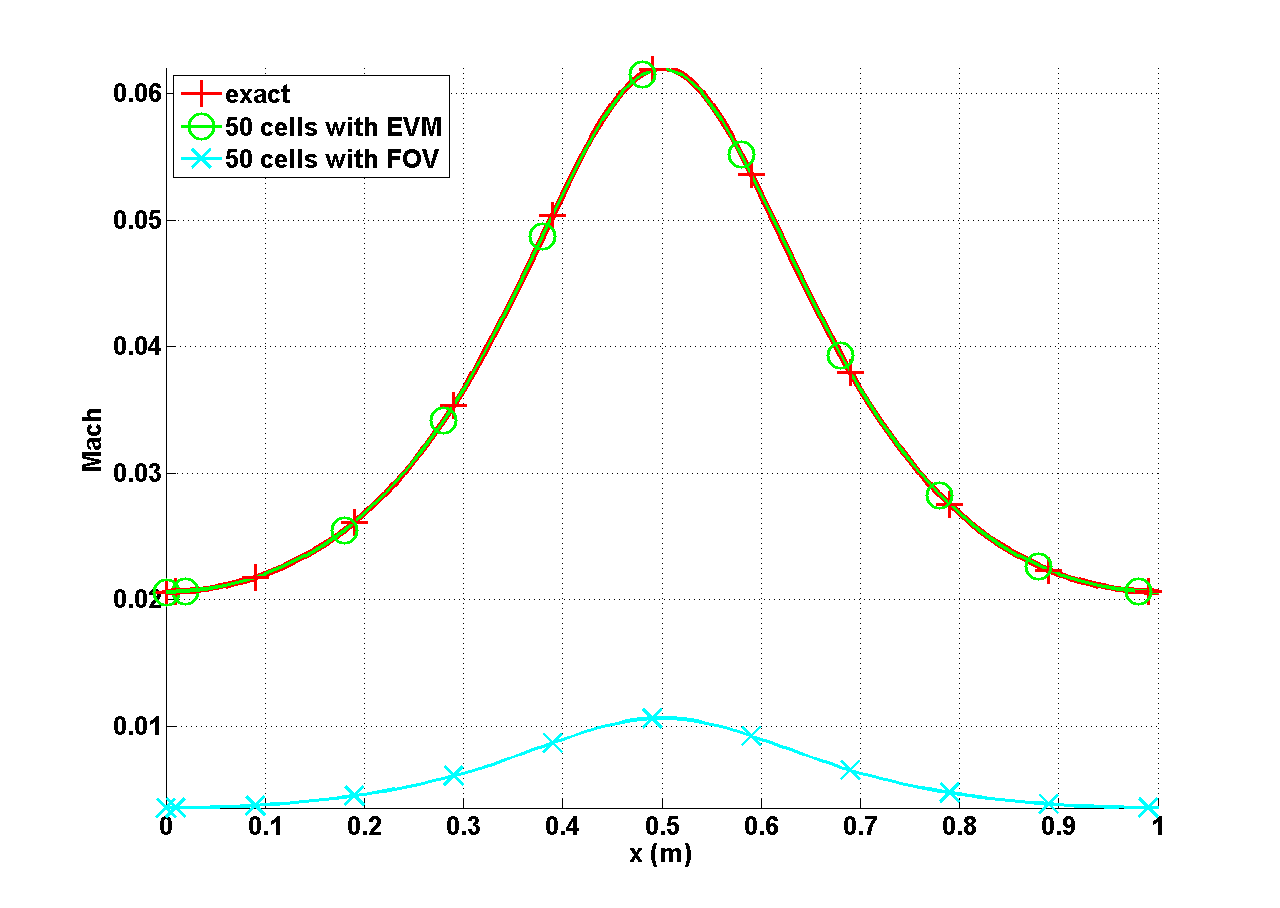
\includegraphics[width=\textwidth]{figures/liquid_mach_numerical_and_exact_50.png}
                \caption{Mach number}
                \label{fig:1d_nozzle_liq_vel}
        \end{subfigure}%
        \begin{subfigure}[b]{0.5\textwidth}
                \centering
                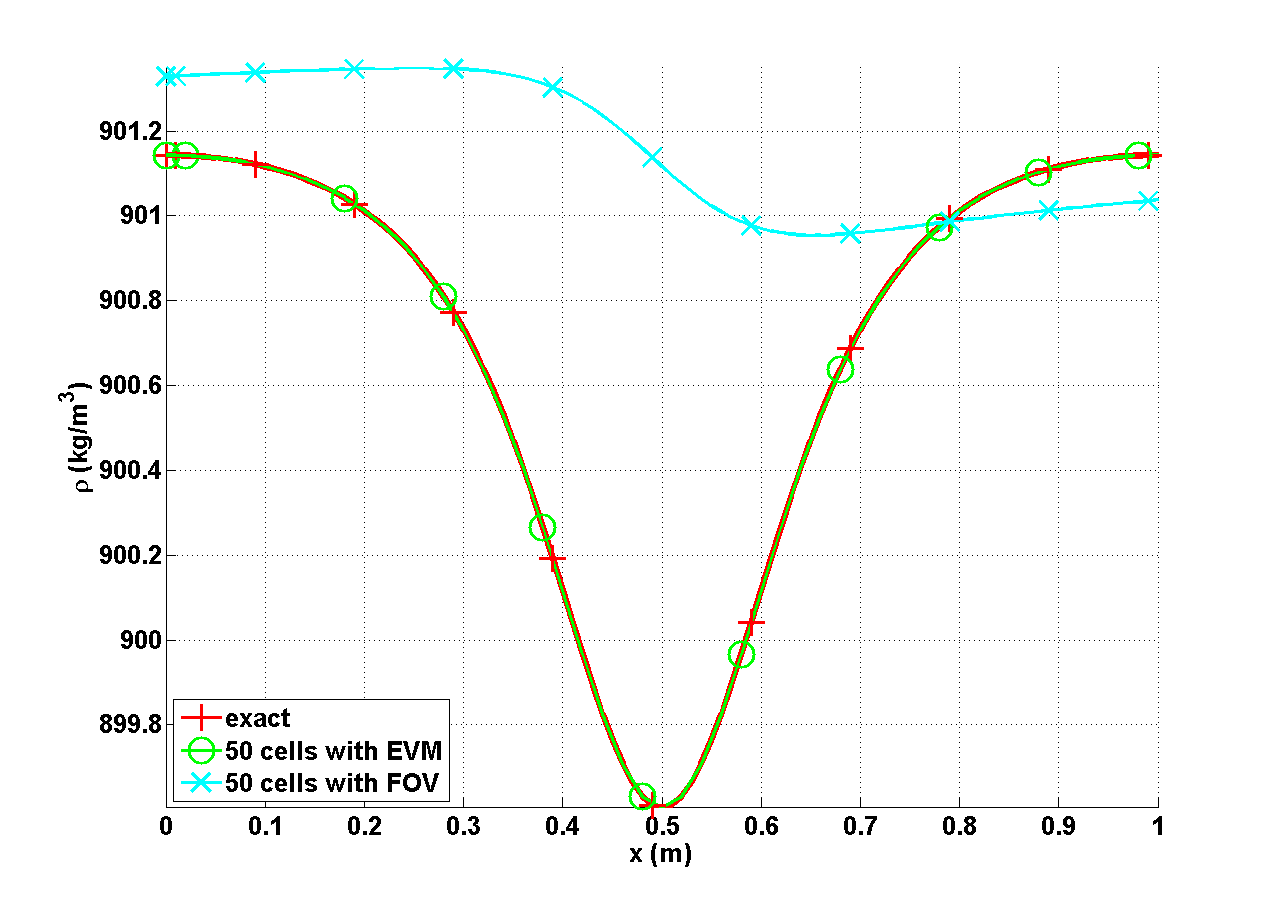
\includegraphics[width=\textwidth]{figures/liquid_density_numerical_and_exact_50.png}
                \caption{Density}
                \label{fig:1d_nozzle_liq_density}
        \end{subfigure}
        
        \begin{subfigure}[b]{0.495\textwidth}
                \centering
                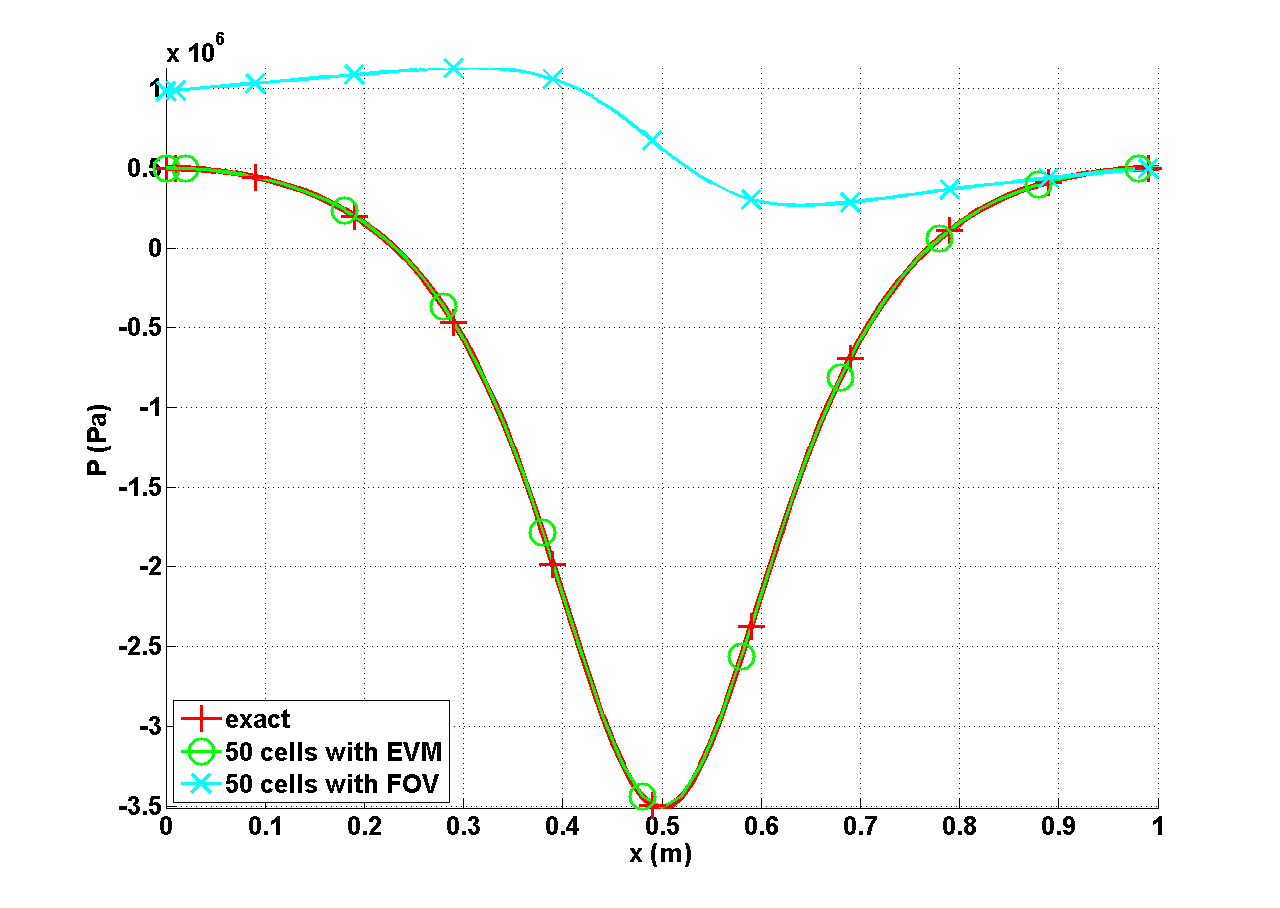
\includegraphics[width=\textwidth]{figures/liquid_pressure_numerical_and_exact_50.png}
                \caption{Pressure}
                \label{fig:1d_nozzle_liq_press}
        \end{subfigure}        
        \begin{subfigure}[b]{0.495\textwidth}
                \centering
                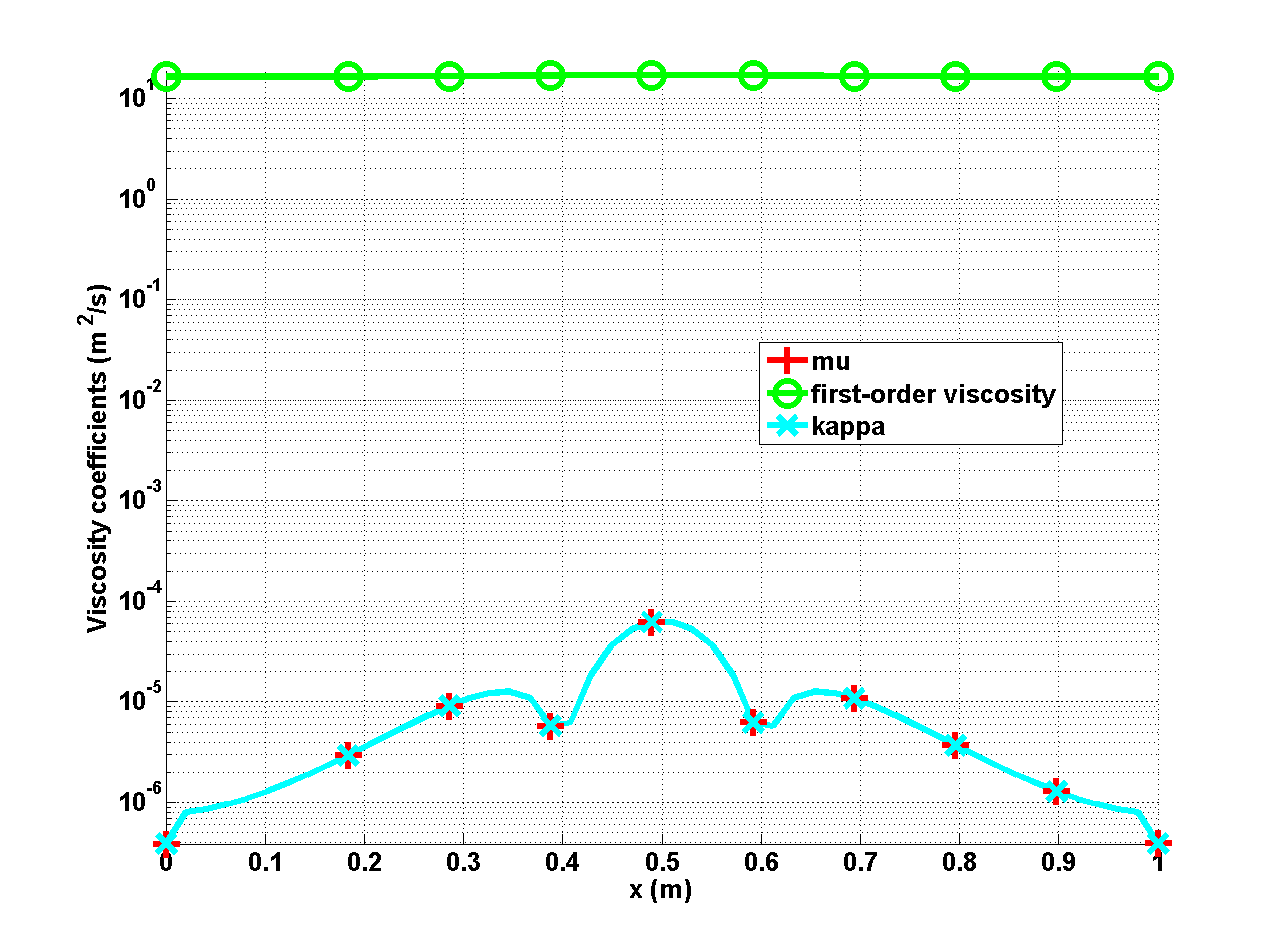
\includegraphics[width=\textwidth]{figures/liquid_viscosity_numerical50.png}
                \caption{Viscosity coefficients}
                \label{fig:1d_nozzle_liq_visc}
        \end{subfigure}
        \caption{Steady-state solution for a liquid flowing through a 1-D converging-diverging nozzle.}\label{fig:1d_liq_nozzle}
\end{figure}
%
In \fig{fig:1d_liq_nozzle}, the numerical solutions obtained using the first-order viscosity (FOV) and the entropy 
viscosity method (EVM) are plotted against the exact solution. The numerical solution obtained with the EVM and the 
exact solution overlap, even for a fairly coarse mesh (50 cells).
On the other hand, the numerical solution obtained with the FOV does not give the correct steady state: this is an 
illustration of the effect of ill-scaled dissipative terms in the low-Mach limit when using the FOV.
%
Note that the entropy viscosity coefficient is very small compared to the first-order one (\fig{fig:1d_nozzle_liq_visc}): 
(i) the numerical solution is smooth as shown in \fig{fig:1d_liq_nozzle} and (ii) the flow is in a isentropic low-Mach regime 
%and thus isentropic 
A convergence study was performed using the exact solution as a reference: the L$_1$ and L$_2$ norms of the 
error and the corresponding convergence rates are computed at steady state on various uniform meshes from 4 to 256 cells.
Spatial convergence results using linear finite elements are reported in \tbl{tbl:l1_norm_liq} and \tbl{tbl:l2_norm_liq} 
for the primitive variables: density, velocity and pressure.
%
\begin{table}[H]
\begin{center}
 \caption{\label{tbl:l1_norm_liq} L$_1$ norm of the error for the liquid phase in a 1-D converging-diverging nozzle at steady state.}
 \begin{tabular}{|c|c|c|c|c|c|c|c|c|}
 \hline
cells & density         & rate   & pressure        & rate    & velocity         & rate     \\ \hline
4    & 2.8037 $10^{-1}$ & $-$    & 8.4705 $10^{5}$ & $-$     & 7.2737           & $-$      \\ \hline
8    & 1.3343 $10^{-1}$ & 1.07 & 4.7893 $10^{5}$ & 0.82 & 6.1493           & 0.24 \\ \hline
16   & 2.9373 $10^{-2}$ & 2.18 & 1.0613 $10^{5}$ & 2.17  & 1.2275           & 2.32   \\ \hline
32   & 5.1120 $10^{-3}$ & 2.52 & 1.8446 $10^{4}$ & 2.52  & 1.8943 $10^{-1}$ & 2.69   \\ \hline
64   & 1.0558 $10^{-3}$ & 2.28 & 3.7938 $10^{3}$ & 2.28  & 3.7919 $10^{-2}$ & 2.32   \\ \hline
128  & 2.3712 $10^{-4}$ & 2.15 & 8.4471 $10^{2}$ & 2.17  & 8.5517 $10^{-3}$ & 2.15   \\ \hline
256  & 5.6058 $10^{-5}$ & 2.08 & 1.9839 $10^{2}$ & 2.09  & 2.0475 $10^{-3}$ & 2.06   \\ \hline
512  & 1.3278 $10^{-5}$ & $2.08$ & 4.6622 $10^{1}$ & 2.09  & 4.9516 $10^{-4}$ & $2.04$   \\ \hline
1024  & 3.1193 $10^{-6}$ & $2.08$ & 1.1755 $10^{1}$ & 1.99  & 1.2379 $10^{-4}$ & 2.00   \\ \hline
\end{tabular}
\end{center}
\end{table}
%
%
\begin{table}[H]
\begin{center}
 \caption{\label{tbl:l2_norm_liq} L$_2$ norm of the error for the liquid phase in a 1-D converging-diverging nozzle at steady state.}
 \begin{tabular}{|c|c|c|c|c|c|c|c|c|}
 \hline
cells& density            & rate & pressure          & rate & velocity           & rate \\ \hline
4    & 3.106397 $10^{-1}$ & $-$  & 5.254445 $10^{5}$ & $-$  & 3.288543           & $-$  \\ \hline
8    & 7.491623 $10^{-2}$ & 2.05 & 1.636966 $10^{5}$ & 1.68 & 1.823880           & 0.85 \\ \hline
16   & 2.079858 $10^{-2}$ & 1.85 & 4.627338 $10^{4}$ & 1.49 & 4.990605 $10^{-1}$ & 0.87 \\ \hline
32   & 5.329627 $10^{-3}$ & 1.96 & 1.180287 $10^{4}$ & 1.97 & 1.261018 $10^{-1}$ & 1.98 \\ \hline
64   & 1.341583 $10^{-3}$ & 1.99 & 2.967104 $10^{3}$ & 1.99 & 3.160914 $10^{-2}$ & 1.99 \\ \hline
128  & 3.359766 $10^{-4}$ & 1.99 & 7.428087 $10^{2}$ & 1.99 & 7.907499 $10^{-3}$ & 1.99 \\ \hline
256  & 8.403859 $10^{-5}$ & 1.99 & 1.857861 $10^{2}$ & 1.99 & 1.977292 $10^{-3}$ & 1.99 \\ \hline
512  & 2.10075  $10^{-5}$ & 2.00 & 4.7024   $10^{1}$ & 1.98 & 4.9516   $10^{-4}$ & 1.99 \\ \hline
\end{tabular}
\end{center}
\end{table}
% \tcr{check the rates in this table as well.} \tcb{I did and changed the values \\}
We note that the convergence rates measured in both the L$_1$ and L$_2$ norm of the error are equal to 2; the entropy viscosity method preserves 
the high-order accuracy of the discretization used when the numerical solution is smooth. The new definition of the entropy viscosity coefficients behaves 
appropriately in the low-Mach limit.

%---------------------------------------------------------------------------------------------------
\subsection{Steam in a 1-D converging-diverging nozzle} \label{sec:steam_nozzle}
%---------------------------------------------------------------------------------------------------

We use the same nozzle geometry, initial conditions and boundary conditions as in the previously example but replace liquid water 
with steam and use the steam parameters of the stiffened gas equation of state, \tbl{tbl:stff_gas_eos}. In this example, 
compressible effects will become dominant. 
The pressure difference between the inlet and outlet is large enough to accelerate the steam through the nozzle, leading 
to the formation of a shock in the diverging portion of the nozzle. The behavior is different from the one observed for the 
liquid water phase in \sct{sec:liquid_nozzle} because of the liquid to gas density ratio is about $1,000$. An exact 
solution at steady state is available for the gas phase \cite{nozzle_exact}. The aim of this section is to show that 
when using the new definitions of the viscosity coefficients (\eqt{eq:final_def_visc_coeff}), the shock can be 
correctly resolved without spurious oscillations. The steady-state numerical solution, obtained using a uniform 
mesh with $500$ cells, is shown in \fig{fig:1d_vap_nozzle}. The $CFL$ was set to $80$ (a high $CFL$ value can be used because the shock is stationary).

\begin{figure}[H]
        \centering
        \begin{subfigure}[b]{0.495\textwidth}
                \centering
                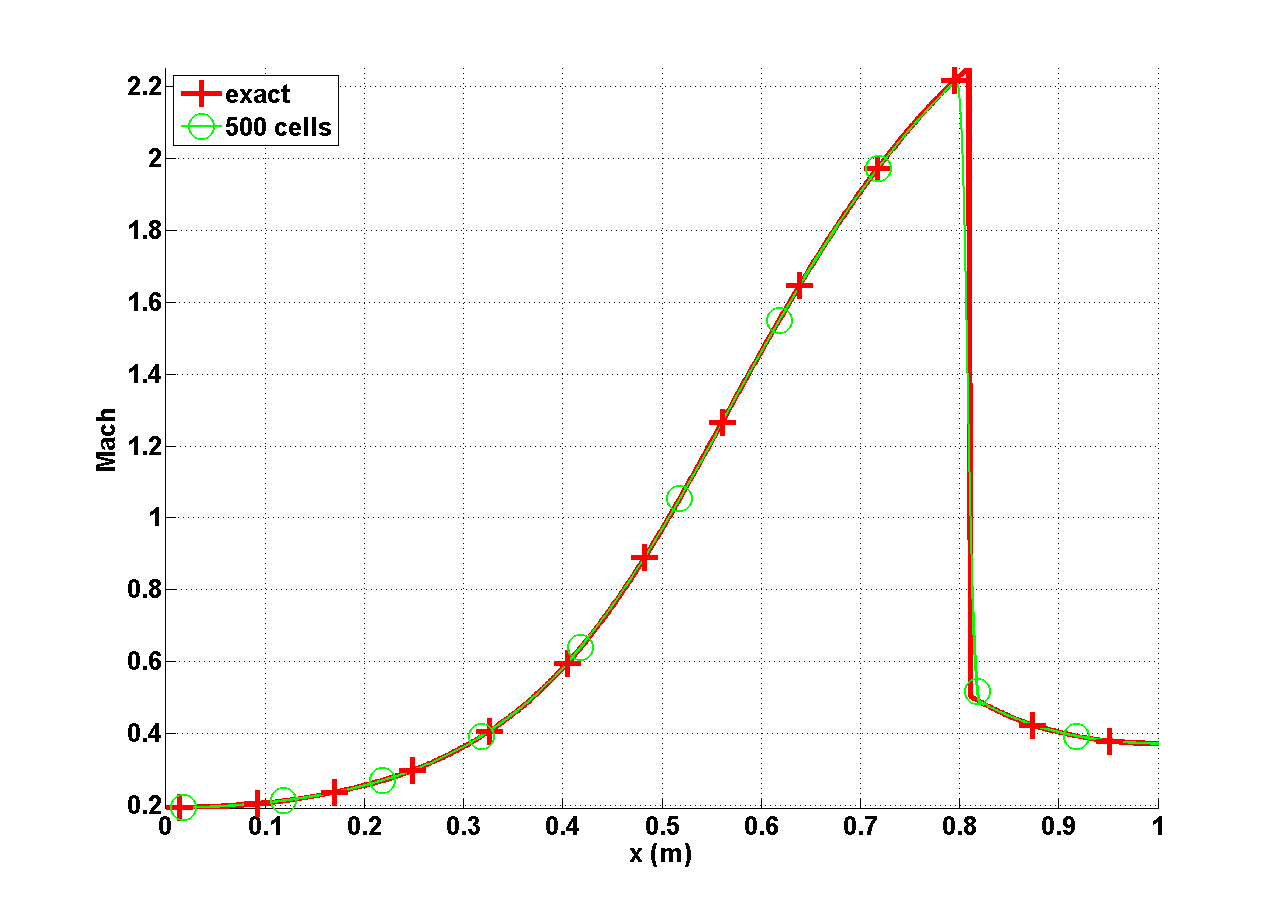
\includegraphics[width=\textwidth]{figures/vapor_mach_numerical_and_exact_500.png}
                \caption{Mach number}
                \label{fig:1d_nozzle_vap_vel}
        \end{subfigure}%
        \begin{subfigure}[b]{0.495\textwidth}
                \centering
                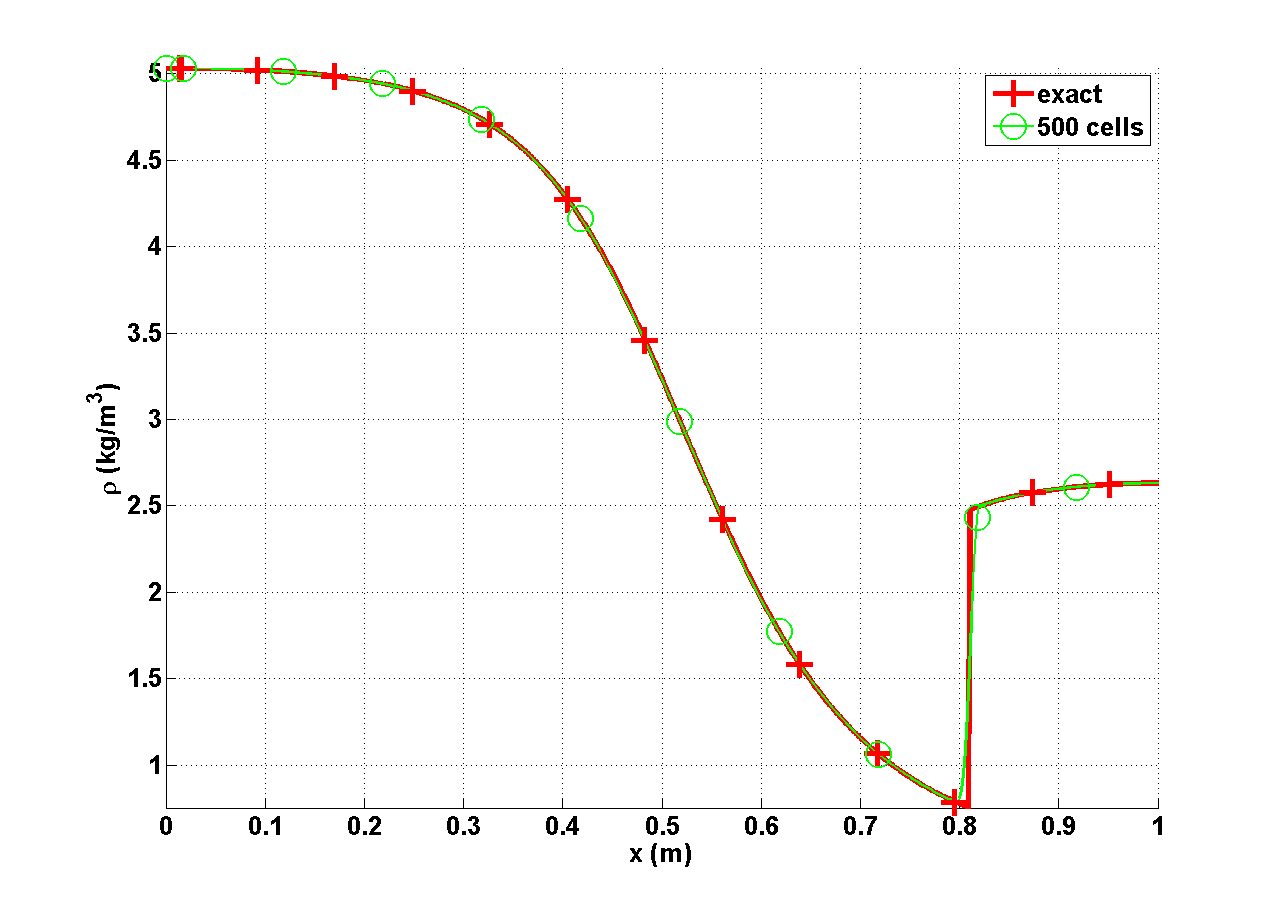
\includegraphics[width=\textwidth]{figures/vapor_density_numerical_and_exact_500.png}
                \caption{Density}
                \label{fig:1d_nozzle_vap_density}
        \end{subfigure}

        \begin{subfigure}[b]{0.495\textwidth}
                \centering
                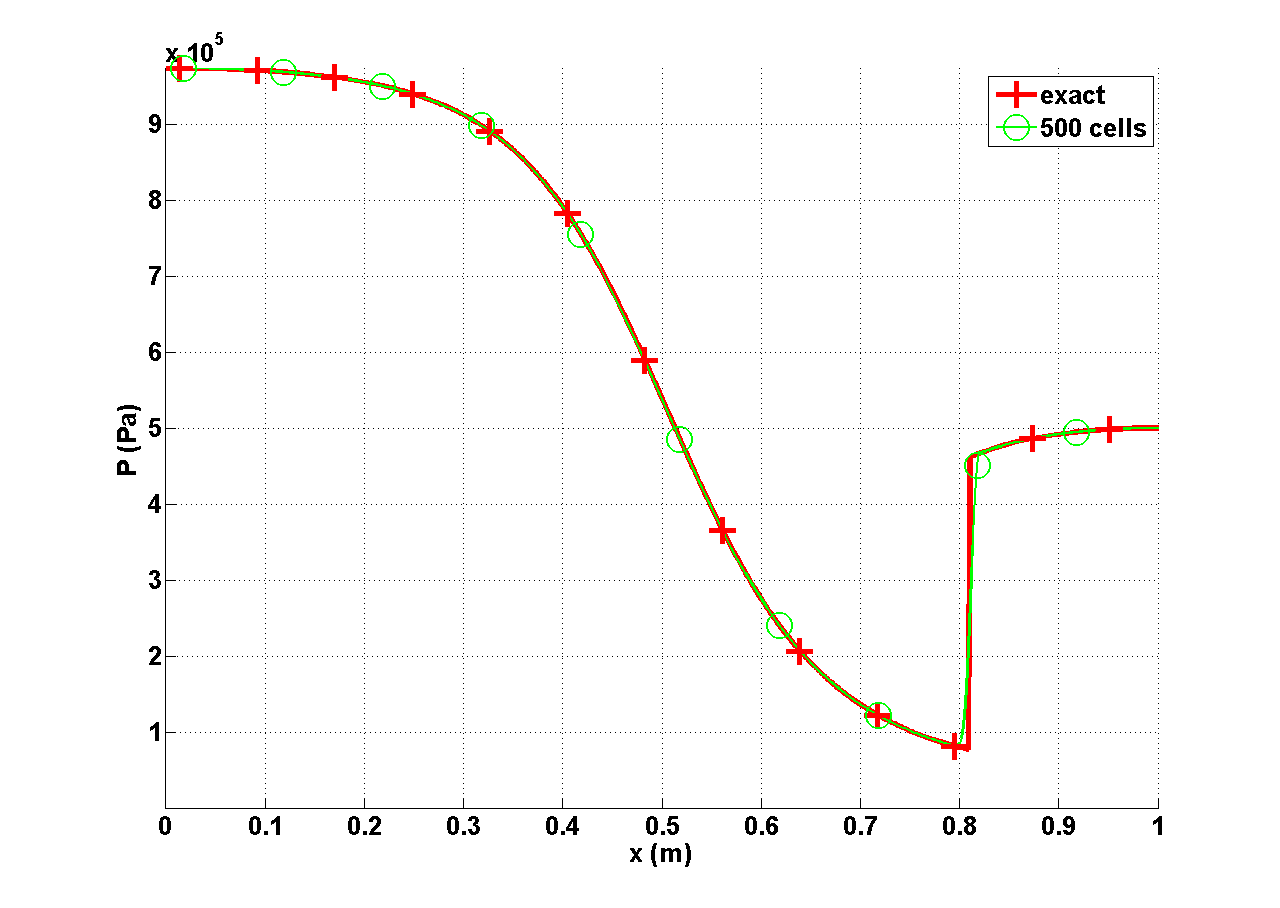
\includegraphics[width=\textwidth]{figures/vapor_pressure_numerical_and_exact_500.png}
                \caption{Pressure}
                \label{fig:1d_nozzle_vap_press}
        \end{subfigure}
        \begin{subfigure}[b]{0.495\textwidth}
                \centering
                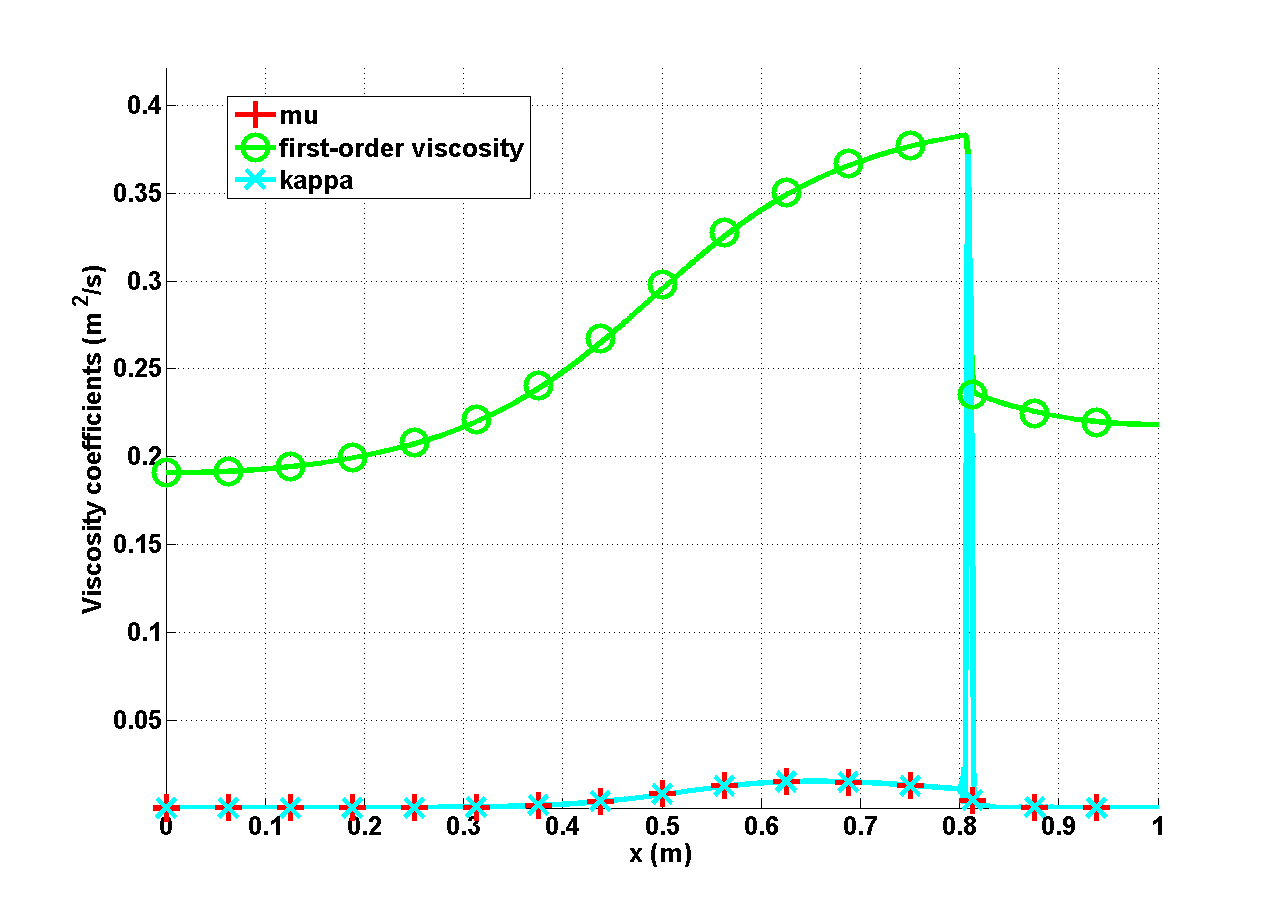
\includegraphics[width=\textwidth]{figures/vapor_viscosity_numerical_500.png}
                \caption{Viscosity coefficients}
                \label{fig:1d_nozzle_vap_visc}
        \end{subfigure}
        \caption{Steady-state solution for vapor phase flowing in a 1-D converging-diverging nozzle.}
				\label{fig:1d_vap_nozzle}
\end{figure}
%
The steady-state solution of the density, Mach number and pressure are given in \fig{fig:1d_vap_nozzle}. 
The steady-state solution exhibits a shock around $x=0.8m$ and matches the exact solution. In \fig{fig:1d_nozzle_vap_visc}, 
the first-order and entropy viscosity coefficients are plotted at steady state (on a log scale): the entropy viscosity 
coefficient is peaked in the shock region around $x=0.8m$ where it saturates to the first-order viscosity 
coefficient. 
%The graph also presents another peak at $x=0.5m$  corresponding to the position of the sonic point for the 
%1-D converging-diverging nozzle. This particular point is known to exhibit small instabilities that are detected when 
%computing the jumps of the pressure and density gradients. 
Elsewhere, the entropy  viscosity coefficient is small. 
In order to prove convergence of the numerical solution to the exact solution, a convergence study is performed. Because 
of the presence of a shock, second-order accuracy is not expected and the convergence rate of a numerical solution 
should be 1 and $1/2$ when measured in the L$_1$ and L$_2$ norms, respectively (see Theorem 9.3 in \cite{convergence_book}). 
Results are reported in \tbl{tbl:l1_norm_vap} and \tbl{tbl:l2_norm_vap} for the primitive variables: density, 
velocity and pressure. The convergence rates for the L$_1$ and L$_2$ norms of the error computed using \eqt{eq:conv_rates} 
are in good agreement with the theoretical values.
%
\begin{table}[!htbp]
\begin{center}
 \caption{\label{tbl:l1_norm_vap} L$_1$ norm of the error for the vapor phase in a 1-D converging-diverging nozzle at steady state.}
 \begin{tabular}{|c|c|c|c|c|c|c|c|c|}
 \hline
cells & density              & rate      & pressure          & rate      & velocity & rate      \\ \hline
$5$  & $0.72562$   $10^{-1}$ & $-$       & $1.5657$ $10^{5}$ & $-$       & $173.69$ & $-$       \\ \hline
$10$ & $0.4165$    $10^{-1}$ & $0.80$ & $9.6741$ $10^{4}$ & $0.63$ & $120.69$ & $0.53$ \\ \hline
$20$ & $0.20675$   $10^{-1}$ & $1.01$  & $4.9193$ $10^{4}$ & $0.97$ & $72.149$ & $0.74$ \\ \hline
$40$ & $0.093703$  $10^{-1}$ & $1.14$  & $2.0103$ $10^{4}$ & $0.73$ & $34.716$ & $1.06$  \\ \hline
$80$ & $0.047328$  $10^{-1}$ & $0.99$  & $1.0208$ $10^{4}$ & $0.98$  & $16.082$ & $1.11$  \\ \hline
$160$& $0.023965$  $10^{-2}$ & $0.98$  & $5.1969$ $10^{3}$ & $0.97$  & $7.9573$ & $1.02$  \\ \hline
$320$& $0.020768$  $10^{-2}$ & $1.03$  & $2.5116$ $10^{3}$ & $1.05$  & $3.7812$ & $1.07$  \\ \hline
$640$& $0.0059715$ $10^{-2}$ & $0.98$  & $1.2754$ $10^{3}$ & $0.98$  & $1.8353$ & $1.04$  \\ \hline
\end{tabular}
\end{center}
\nonumber
\end{table}
%\tcr{I was NOT able to reproduce all of the L1 density convergence rates with the 2-pt formula. I have\\
%         0.800897725302031\\
%          1.01042916619427\\
%          1.14172018626244\\
%         0.985401280471854\\
%          4.30369311248011\\
%         0.206566651507186\\
%          1.79819701118663\\
%My last 3 rates are wrong. 	It could be because you table does not give enough digits but you give many digits so please investigate this.}

\begin{table}[H]
\begin{center}
 \caption{\label{tbl:l2_norm_vap} L$_2$ norm of the error for the vapor phase in a 1-D converging-diverging nozzle at steady state.}
 \begin{tabular}{|c|c|c|c|c|c|c|c|c|}
 \hline
cells & density             & rate      & pressure          & rate      & velocity & rate       \\ \hline
$5$   & $9.7144$ $10^{-1}$  & $-$       & $2.0215$ $10^{5}$ & $-$       & $236.94$ & $-$        \\ \hline
$10$  & $5.9718$ $10^{-1}$  & $0.70$ & $1.3024$ $10^{5}$ & $0.63$ & $166.56$ & $0.51$  \\ \hline
$20$  & $2.9503$ $10^{-1}$  & $1.02$  & $6.6503$ $10^{4}$ & $0.97$ & $103.36$ & $0.69$  \\ \hline
$40$  & $1.8193$ $10^{-1}$  & $0.69$ & $4.0171$ $10^{4}$ & $0.73$ & $66.374$ & $0.64$   \\ \hline
$80$  & $1.3366$ $10^{-1}$  & $0.44$ & $2.3163$ $10^{4}$ & $0.44$ & $42.981$ & $0.63$  \\ \hline
$160$ & $9.6638$ $10^{-2}$  & $0.47$ & $1.7263$ $10^{4}$ & $0.42$ & $31.717$ & $0.44$  \\ \hline
$320$ & $7.0896$ $10^{-2}$  & $0.45$ & $1.2763$ $10^{4}$ & $0.44$ & $23.138$ & $0.45$  \\ \hline
$640$ & $5.2191$ $10^{-2}$  & $0.44$ & $9.4217$ $10^{3}$ & $0.44$ & $16.910$ & $0.45$  \\ \hline
\end{tabular}
\end{center}
\nonumber
\end{table}
%\tcr{I was able to reproduce the L2 density convergence rate with the 2-pt formula. Table 6 is Ok}
%---------------------------------------------------------------------------------------------------
\subsection{Leblanc shock tube} \label{sec:Leblanc}
%---------------------------------------------------------------------------------------------------

The 1-D Leblanc shock tube is a Riemann problem designed to test the robustness and the accuracy of stabilization methods. 
The initial conditions are given in \tbl{tbl:ic_1d_tests}. The ideal gas equation of state (with $\gamma=5/3$) is used to 
compute the pressure.
This test is computationally challenging because of the large pressure ratio at the initial interface.
The computational domain consists of a 1-D straight pipe of length $L=9m$ with the initial interface located at $x=2m$. 
At $t=0\,s$, the interface is removed. The numerical solution is run until $t=4\,s$ and the density, momentum and 
total energy profiles are given in \fig{fig:1d_leblanc}, along with the exact solution. The viscosity coefficients 
are also plotted in \fig{fig:1d_leblanc_visc}. These plots were run with three different uniform meshes of $800$, 
$3200$, and $6000$ cells and a constant $CFL = 1$.
\begin{figure}[H]
        \centering
        \begin{subfigure}[b]{0.495\textwidth}
                \centering
                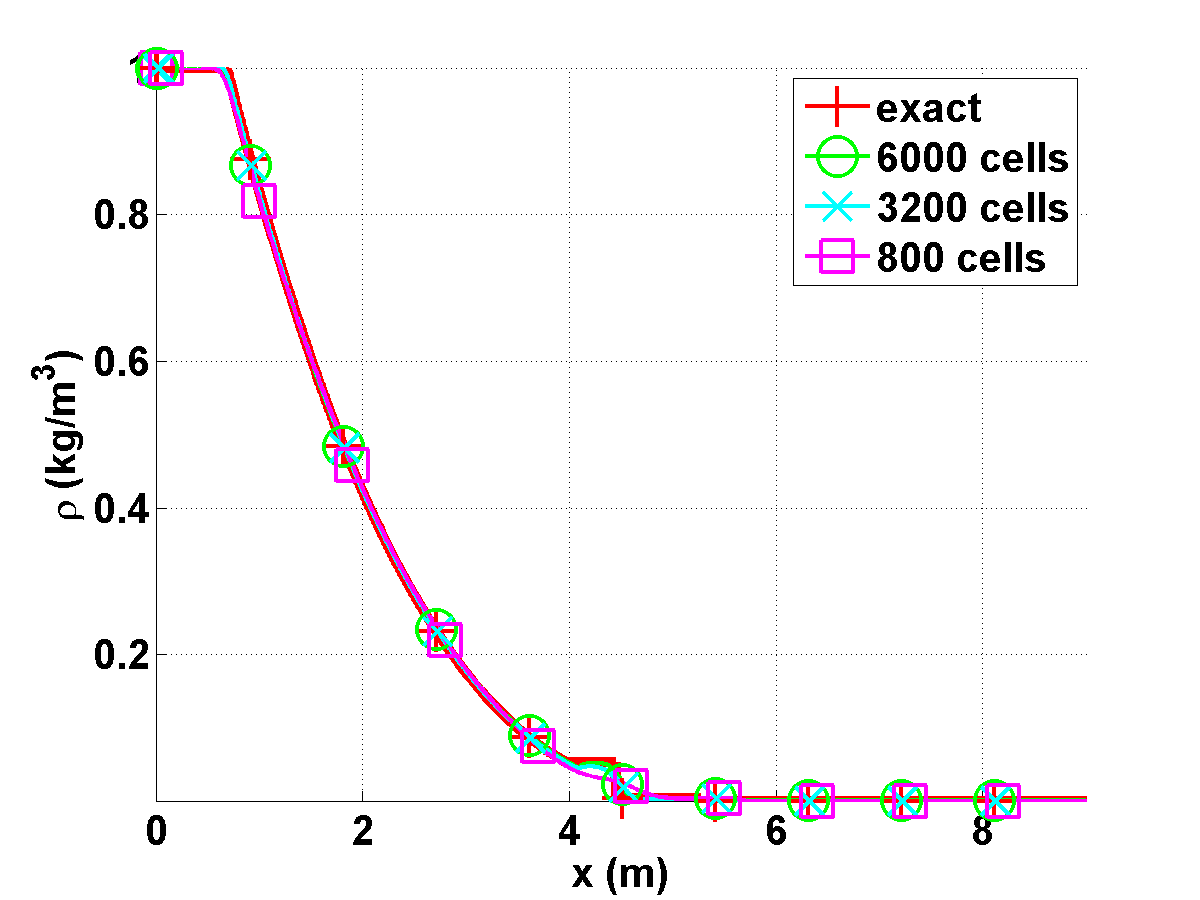
\includegraphics[width=\textwidth]{figures/Leblanc_exact_and_numerical_stt_density_6000.png}
                \caption{Density}
                \label{fig:1d_leblanc_vel}
        \end{subfigure}%
        %add desired spacing between images, e. g. ~, \quad, \qquad etc. 
          %(or a blank line to force the subfigure onto a new line)
        \begin{subfigure}[b]{0.495\textwidth}
                \centering
                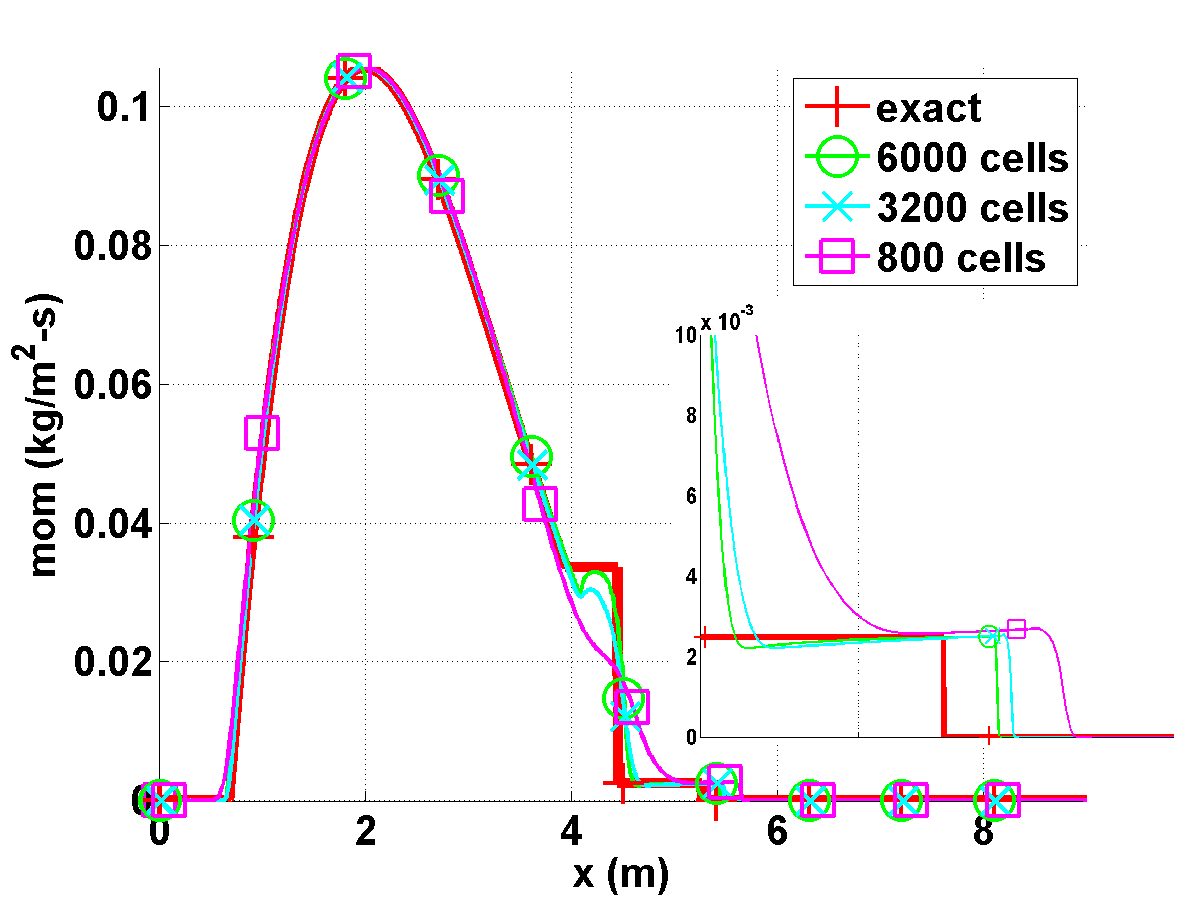
\includegraphics[width=\textwidth]{figures/Leblanc_exact_and_numerical_stt_momentum_6000.png}
                \caption{Momentum}
                \label{fig:1d_leblanc_density}
        \end{subfigure}
         %add desired spacing between images, e. g. ~, \quad, \qquad etc. 
          %(or a blank line to force the subfigure onto a new line)
        \begin{subfigure}[b]{0.495\textwidth}
                \centering
                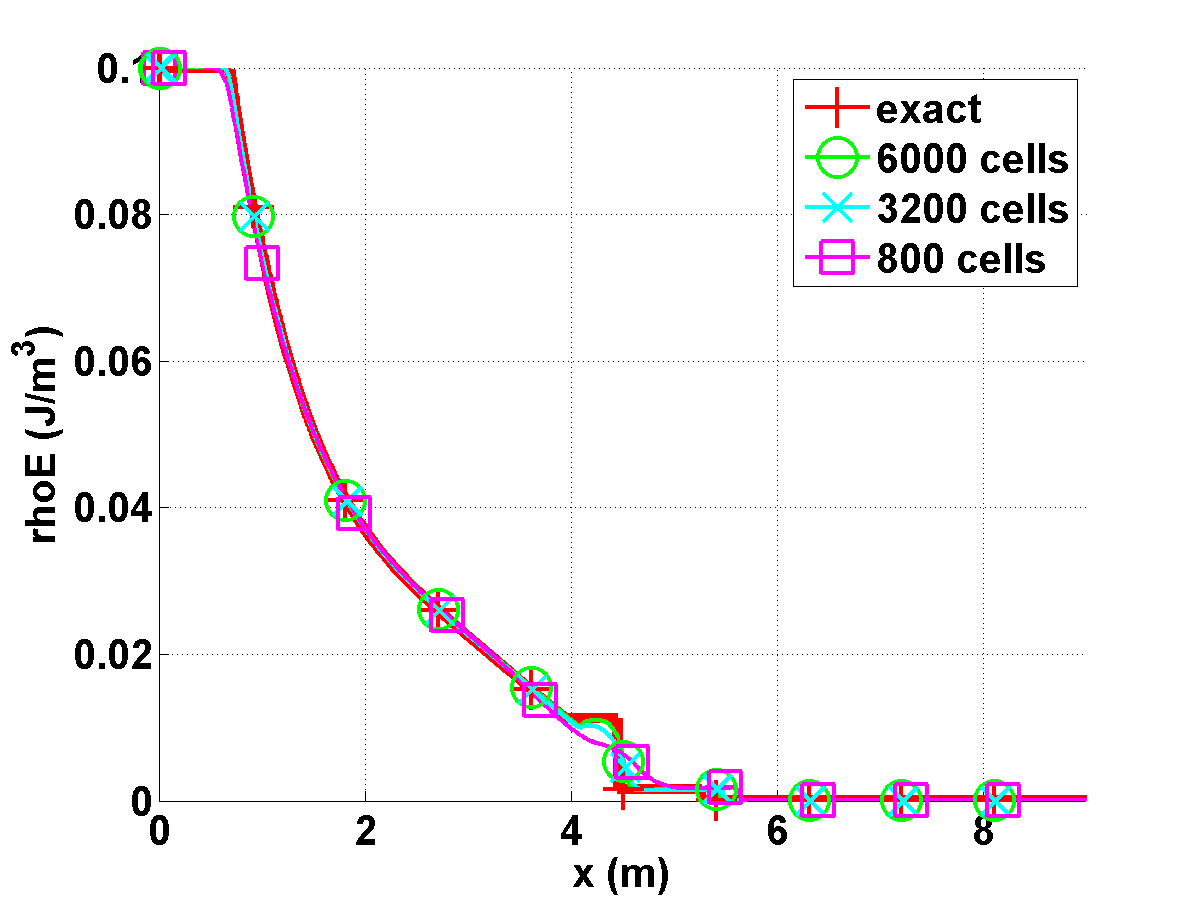
\includegraphics[width=\textwidth]{figures/Leblanc_exact_and_numerical_stt_total_energy_6000.png}
                \caption{Total energy}
                \label{fig:1d_leblanc_press}
        \end{subfigure}
          %add desired spacing between images, e. g. ~, \quad, \qquad etc. 
          %(or a blank line to force the subfigure onto a new line)
        \begin{subfigure}[b]{0.495\textwidth}
                \centering
                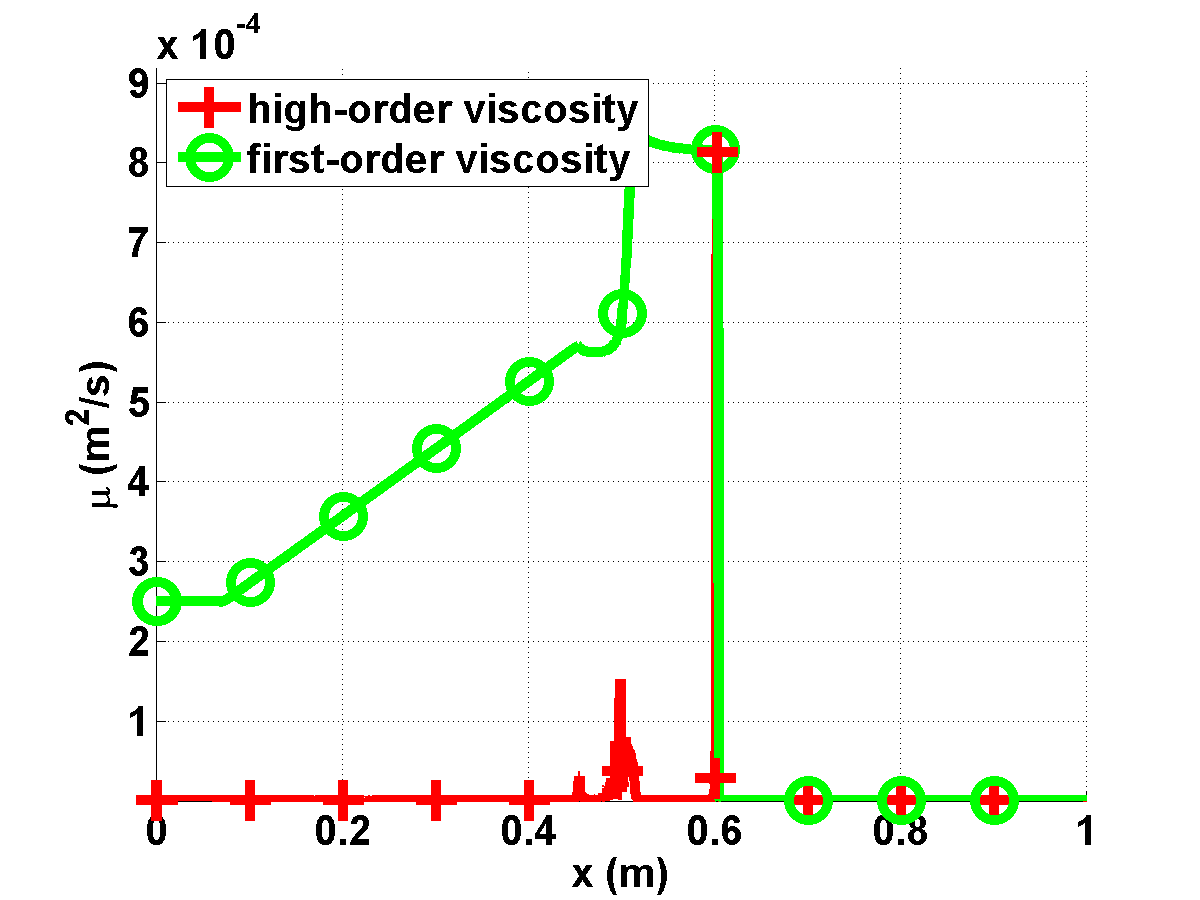
\includegraphics[width=\textwidth]{figures/Leblanc_viscosity_numerical_6000.png}
                \caption{Viscosity coefficients}
                \label{fig:1d_leblanc_visc}
        \end{subfigure}
        \caption{Exact and Numerical solutions for the 1-D Leblanc shock tube at $t=4\,s$.}\label{fig:1d_leblanc}
\end{figure}
%
The density, momentum and total energy profiles are provided in \fig{fig:1d_leblanc}. In \fig{fig:1d_leblanc_density}, 
the shock region is zoomed in for better resolution: the shock is well resolved. We also observe that the shock 
position computed numerically converges to the exact position under mesh refinement. The contact wave at $x=4.5m$ 
can be seen in \fig{fig:1d_leblanc_density}. The entropy viscosity coefficient profile is shown in 
\fig{fig:1d_leblanc_visc} and behaves as expected: it saturates to the first-order viscosity in the 
shock region, thus preventing oscillations from forming. At the location of the contact wave, a 
smaller peak is observed and is due to the presence of the jump terms in the definition of the entropy 
viscosity coefficient (\eqt{eq:final_def_visc_coeff}).  The Mach number, not plotted, is of the order 
of $1.3$ just before the shock and reaches a maximum value close to $5$ in the contact region.

Once again, a convergence study is performed in order to prove convergence of the numerical solution to 
the exact solution. As in the previous example (vapor phase in the 1-D nozzle, \sct{sec:steam_nozzle}), 
the expected convergence rates in the L$_1$ and L$_2$ norms are 1 and $1/2$, respectively. The exact 
solution was obtained by running a 1-D Riemann solver and used as the reference solution to compute 
the L$_1$ and L$_2$-norms that are reported in \tbl{tbl:l1_norm_leblanc} and \tbl{tbl:l2_norm_leblanc} 
for the conservative variables: density, momentum and total energy. The convergence rates are again approaching their theoretical values.

\begin{table}[!htbp]
\begin{center}
 \caption{\label{tbl:l1_norm_leblanc} L$_1$ norm of the error for the 1-D Leblanc test at $t=4s$.}
 \begin{tabular}{|c|c|c|c|c|c|c|c|c|}
 \hline
  cells & density               & rate         & momentum              & rate          & total energy          & rate         \\  \hline
$100$   & $1.0354722$ $10^{-2}$ & $-$          & $3.5471714$ $10^{-3}$ & $-$           & $1.4033046$ $10^{-3}$ & $-$          \\  \hline
$200$   & $7.2680512$ $10^{-3}$ & $0.51$ & $2.5933119$ $10^{-3}$ & $0.45$  & $9.8611746$ $10^{-4}$ & $0.51$  \\  \hline
$400$   & $5.0825628$ $10^{-3}$ & $0.52$ & $2.0668092$ $10^{-3}$ & $0.33$  & $7.7844421$ $10^{-4}$ & $0.34$ \\  \hline
$800$   & $3.4025056$ $10^{-3}$ & $0.58$ & $1.4793838$ $10^{-3}$ & $0.48$  & $5.5702549$ $10^{-4}$ & $0.48$ \\  \hline
$1600$  & $2.1649953$ $10^{-3}$ & $0.65$ & $9.7152832$ $10^{-4}$ & $0.61$   & $3.5720171$ $10^{-4}$ & $0.64$ \\  \hline
$3200$  & $1.2465433$ $10^{-3}$ & $0.79$ & $5.5937409$ $10^{-4}$ & $0.79$  & $2.0491799$ $10^{-4}$ & $0.80$ \\  \hline
$6400$  & $6.4476928$ $10^{-4}$ & $0.95$ & $3.0244198$ $10^{-4}$ & $0.89$  & $1.0914891$ $10^{-4}$ & $0.91$ \\  \hline
$12800$ & $3.3950948$ $10^{-4}$ & $0.93$ & $1.5958118$ $10^{-4}$ & $0.92$   & $5.7909794$ $10^{-5}$ & $0.91$ \\  \hline
 \end{tabular}
\end{center}
\end{table}
%
\begin{table}[!htbp]
\begin{center}
 \caption{\label{tbl:l2_norm_leblanc} L$_2$ norm of the error for the 1-D Leblanc test at $t=4s$.}
 \begin{tabular}{|c|c|c|c|c|c|c|}
 \hline
   cells & density & rate & momentum & rate & total energy & rate \\ \hline
$100$ &   $5.7187851$ $10^{-3}$ & $-$ & $1.7767236$ $10^{-3}$ & $-$ & $7.6112265$  $10^{-4}$& $-$\\   \hline
$200$  &  $3.8995238$ $10^{-3}$ & $0.55$ & $1.4913161$ $10^{-3}$ & $0.25$ &  $5.5497308$ $10^{-4}$& $0.46$\\ \hline
$400$ & $2.8103526$ $10^{-3}$   & $0.47$ & $1.3305301$ $10^{-3}$ & $0.16$ & $4.6063172$ $10^{-4}$ & $0.27$\\ \hline
$800$ & $2.1081933$ $10^{-3}$   & $0.41$ & $1.1398931$ $10^{-3}$ & $0.22$ & $3.7798953$ $10^{-4}$ & $0.29$\\ \hline
$1600$ & $1.5731052$ $10^{-3}$  & $0.42$ & $9.0394227$ $10^{-4}$ & $0.33$ & $2.9584646$ $10^{-4}$ & $0.35$\\ \hline
$3200$&$1.0610667$ $10^{-3}$    & $0.57$ & $6.2735595$ $10^{-4}$ & $0.53$ & $2.054455$ $10^{-4}$ & $0.53$\\ \hline
$6400$&$7.3309974$ $10^{-4}$    & $0.53$ & $4.4545754$ $10^{-4}$ & $0.49$ & $1.4670834$ $10^{-4}$ & $0.49$\\ \hline
 $12800$&$5.1020991$ $10^{-4}$  & $0.52$ & $3.1266758$ $10^{-4}$ & $0.51$ & $1.0299897$ $10^{-5}$ & $0.51$\\  \hline
\end{tabular}
\end{center}
\nonumber
\end{table}

%---------------------------------------------------------------------------------------------------
\subsection{1-D shock tube with a liquid phase} \label{sec:liquid_shock}
%---------------------------------------------------------------------------------------------------
%\tcr{until now, you never gave the mu and kappa coefficients, yet they are now different due to their different normalizations.
%Maybe very little for the previous cases, but we need to mention something because, in this section, you show both, and it is better
%to say something than to let the reviewers wonder ... } \tcb{what do you think of the following?}
The purpose of this test is to investigate the ability of the entropy viscosity method to stabilize a strong 
shock with a small Mach number \cite{abgrall} (this reference is for a two-phase flow model but we are only 
interested in the initial conditions for the liquid phase): the Mach number in the shock region is of the 
order of 0.1. In this case, as explained in \sct{sec:lowMach}, the viscosity coefficients are required to 
have different order of magnitude in order to ensure the correct scaling of the dissipative terms. 
The purpose of this test is to validate the approach presented in \sct{sec:lowMach}. 

The stiffened gas equation of state is used to model a liquid flow with the parameters given in 
\tbl{tbl:stff_gas_eos}. The computational domain of length $L=1m$ is uniformly discretized using 500 cells. 
The step initial conditions are given in \tbl{tbl:ic_1d_tests}.
%
The simulation is run with a $CFL=1$ until the final time $t_{\text{final}} = 7 \ 10^{-5}s$. Results 
for pressure, density, velocity and the viscosity coefficients are given in \fig{fig:1d_strong_shock} 
along with the exact solution for comparison purposes. The numerical solution is in good agreement 
with exact solution in \fig{fig:1d_strong_shock_var}. The viscosity coefficients $\mu$ and $\kappa$ 
are not equal in the shock because the Mach number is of order $0.1$. The viscosity coefficient $\kappa$ 
saturates to the first-order viscosity in the shock region around $x = 0.65m$ and is sufficient to 
stabilize the numerical scheme. 
%This example illustrates the capabilities of the entropy viscosity method to stabilize a strong shock using liquid fluid properties. 
%
\begin{figure}[H]
        \centering
        \begin{subfigure}[b]{0.495\textwidth}
                \centering
                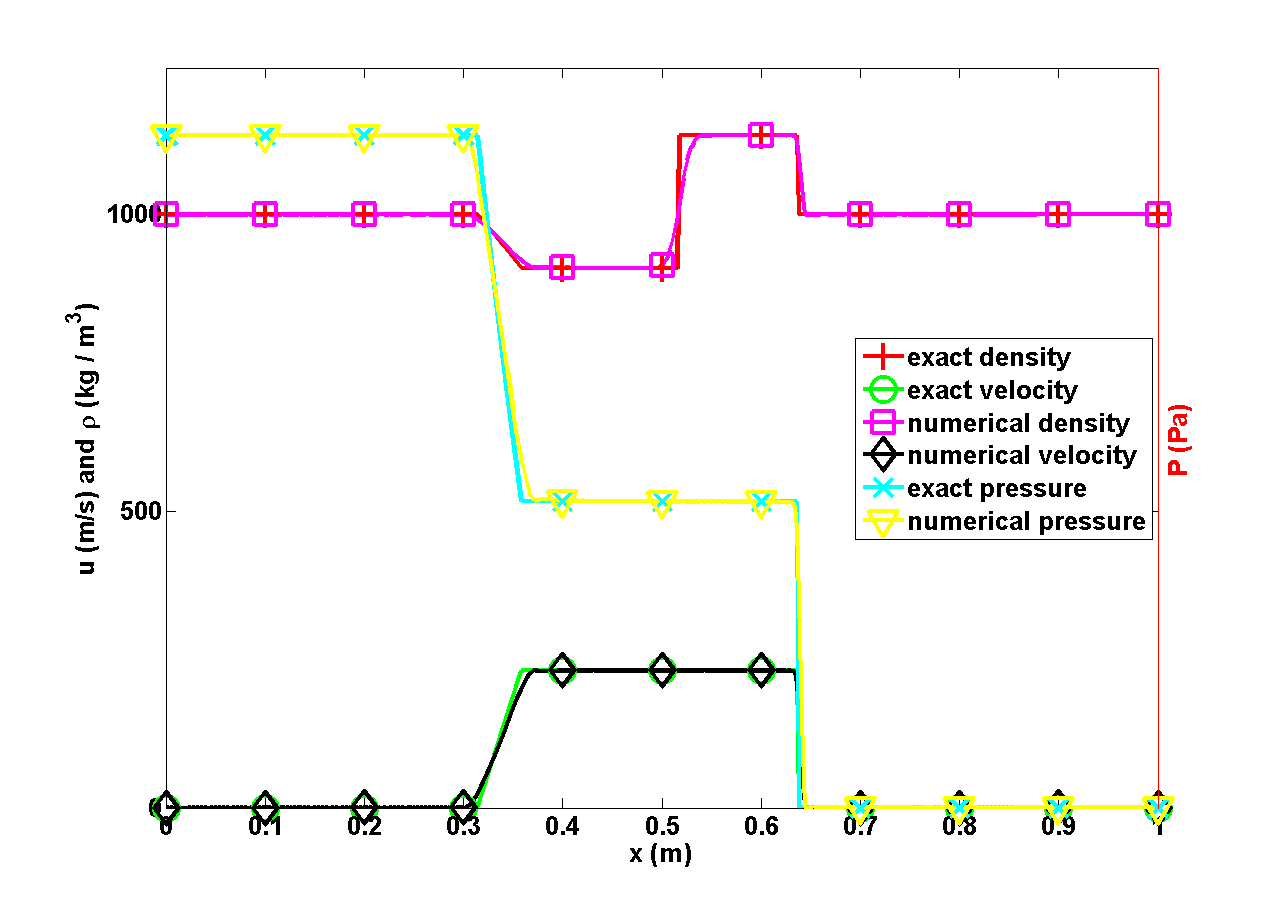
\includegraphics[width=\textwidth]{figures/LiquidSrongShock_density_velocity_pressure_profiles.png}
                \caption{Density, velocity and pressure profiles.}
                \label{fig:1d_strong_shock_var}
        \end{subfigure}%
        \begin{subfigure}[b]{0.495\textwidth}
                \centering
                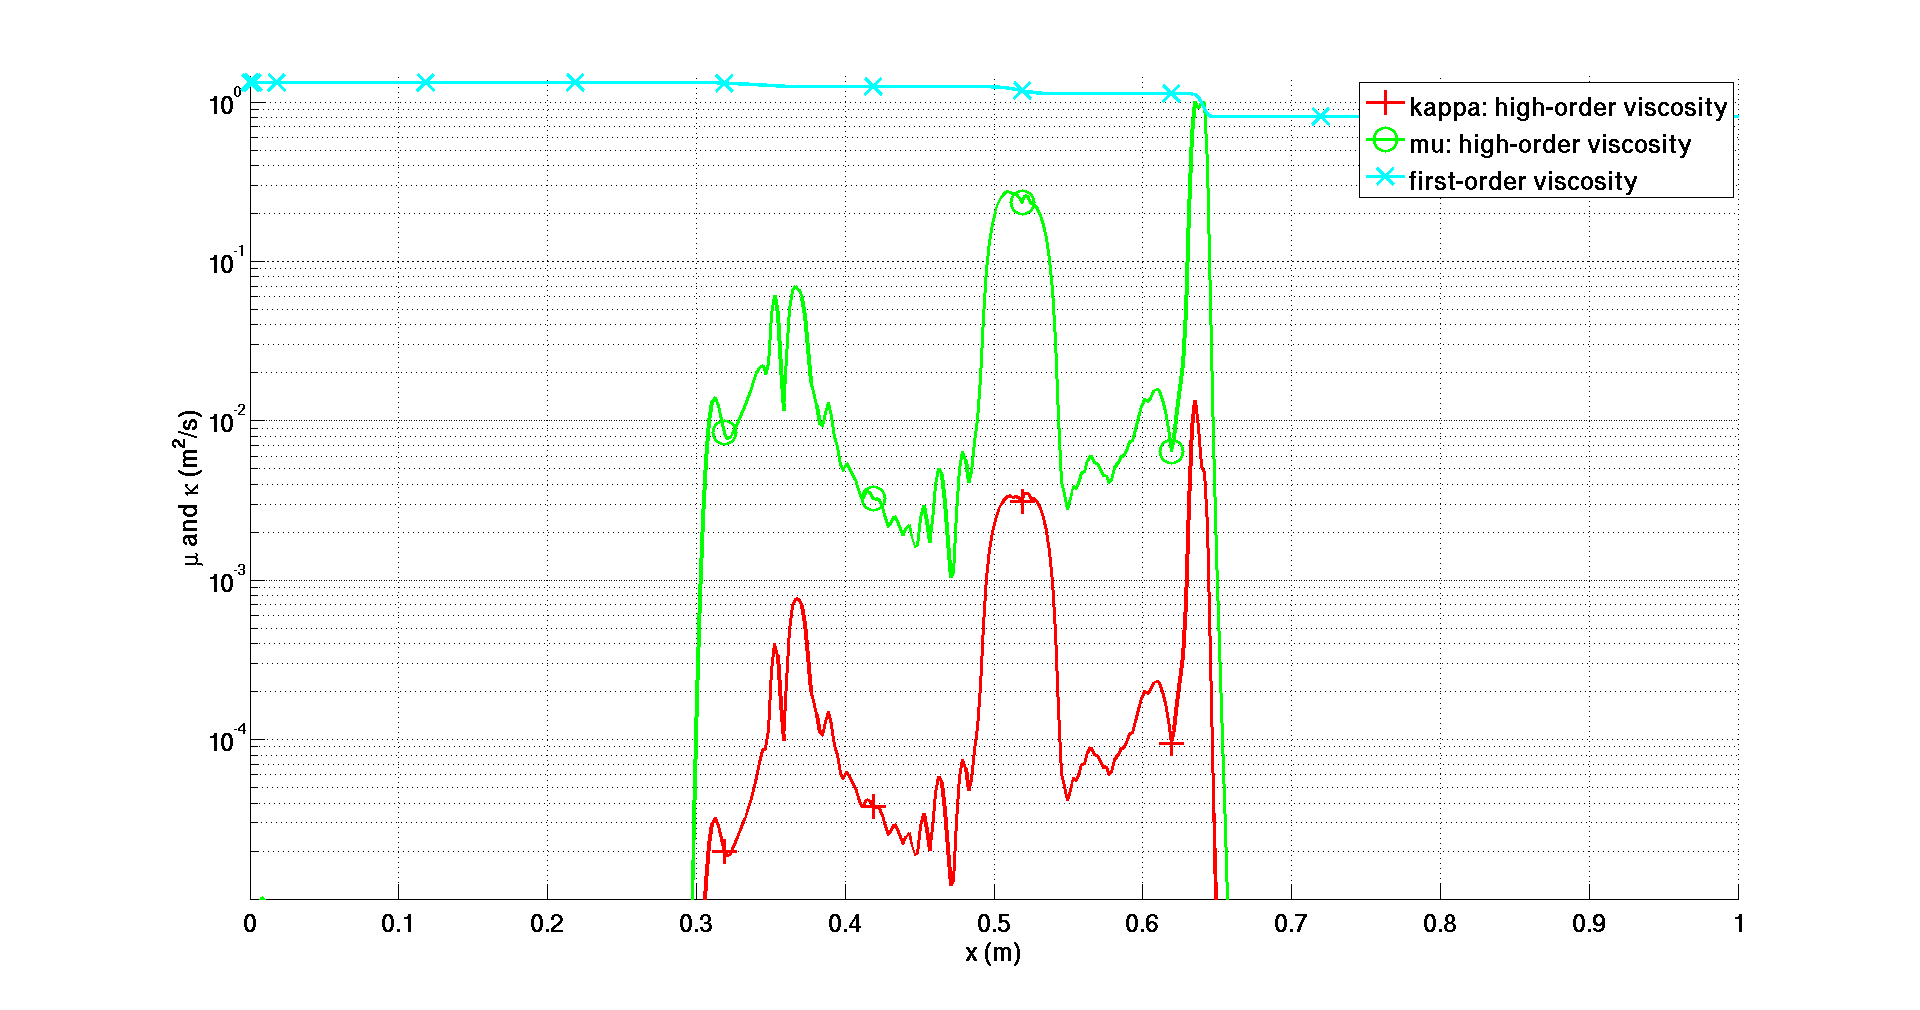
\includegraphics[width=\textwidth]{figures/LiquidSrongShock_viscosity.png}
                \caption{Viscosity coefficients profile.}
                \label{fig:1d_strong_shock_visc}
        \end{subfigure}
        \caption{Numerical solution for the 1-D liquid shock tube at  at $t_{\text{final}} = 7 \  10^{-5}s$.}
				\label{fig:1d_strong_shock}
\end{figure}


%---------------------------------------------------------------------------------------------------
\subsection{1-D slow moving shock} \label{sec:slow_moving_shock}
%---------------------------------------------------------------------------------------------------

Slow moving shocks are known to produce post-shock noise of low frequency that is not damped by some 
numerical dissipation methods \cite{james}. The aim of this simulation is to test the ability of the 
entropy viscosity method to dampen the low frequency waves.
The 1-D slow moving shock consists of a shock wave moving from left to right with the initial conditions 
given in \tbl{tbl:ic_1d_tests}. The ideal gas equation of state is used with a heat capacity ratio 
$\gamma=1.4$.  In order to make the shock travel a significant distance, the final time is taken 
equal to $t=1.1\,s$. A pressure boundary condition is used at the left boundary to let the rarefaction 
and contact waves exit the domain.   
%
The numerical solution, obtained with 200 equally-spaced cells, is given in \fig{fig:low_moving_shock} 
and is compared to the exact solution obtained from a Riemann solver. We use a $CFL$ of 1. With this 
$CFL$ value, it takes about 50 time steps for the shock to traverse one cell.
%
The numerical results are in good agreement with the exact solution and do not display any post-shock 
noise. The rarefaction and contact waves are not visible on \fig{fig:profiles_sms} since they exited 
the computational domain through the left pressure boundary condition earlier. As explained in 
\cite{roberts}, Godunov's type methods usually fail to resolve a slow moving shock because of the 
nature of the stabilization method: the method scales as the eigenvalue of the appropriate field. 
In the case of a slow moving shock, the dissipation added to the system is under-estimated and leads 
to post-shock noise. In the case of the entropy viscosity method, the entropy residual detects 
the shock position and the viscosity coefficients saturate to the first-order viscosity values in 
the shock region. The main difference between a  Godunov's type method and the entropy viscosity 
method lies in the definition of the first-order viscosity coefficients that are proportional to 
the \emph{local maximum eigenvalue} $||\vec{u}||+c$ and not to the eigenvalue of the characteristic field.
%
\begin{figure}[H]
        \centering
        \begin{subfigure}[b]{0.495\textwidth}
                \centering
                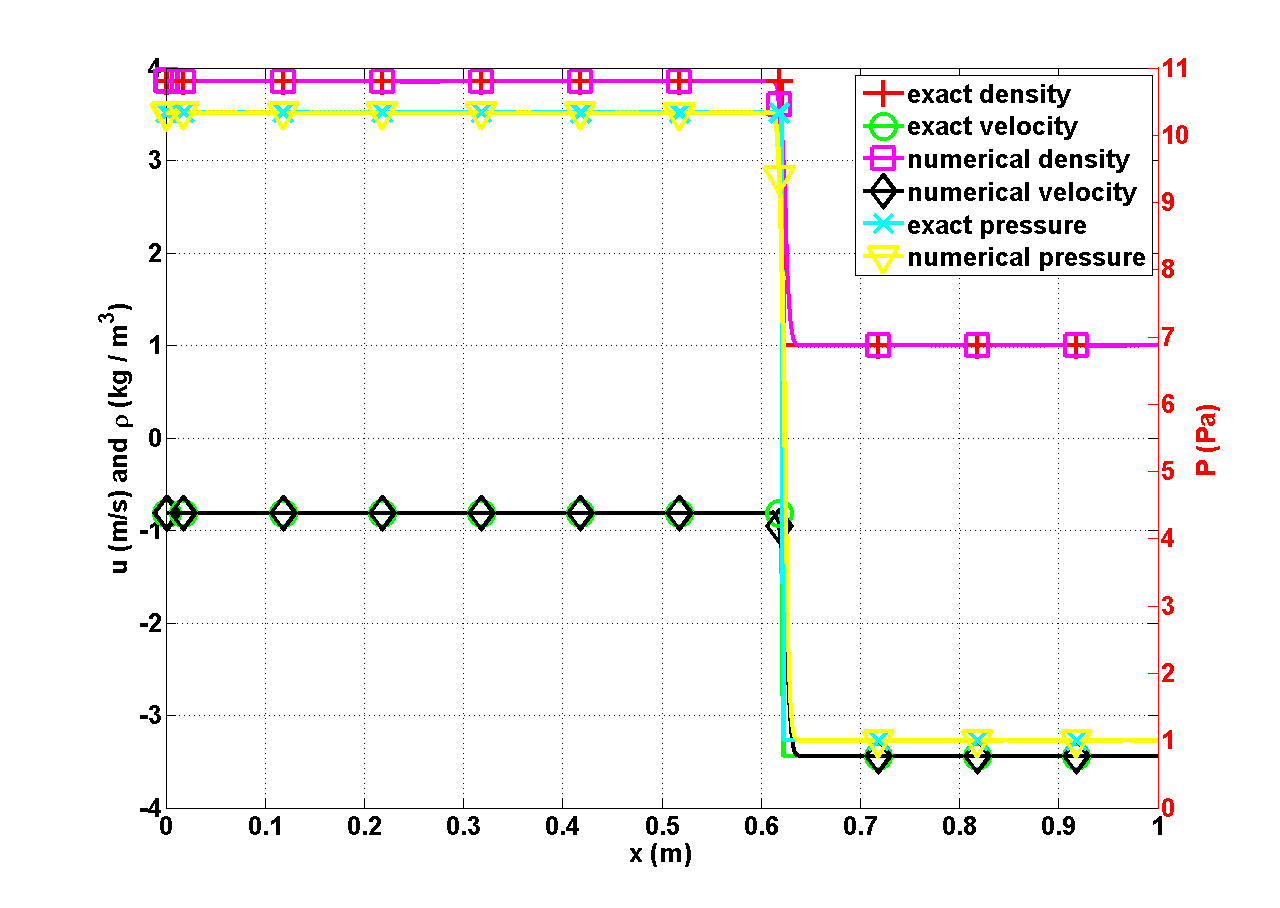
\includegraphics[width=\textwidth]{figures/SlowMovingShock_density_velocity_pressure_profiles.png}
                \caption{Velocity, density and pressure}
                \label{fig:profiles_sms}
        \end{subfigure}%
        \begin{subfigure}[b]{0.495\textwidth}
                \centering
                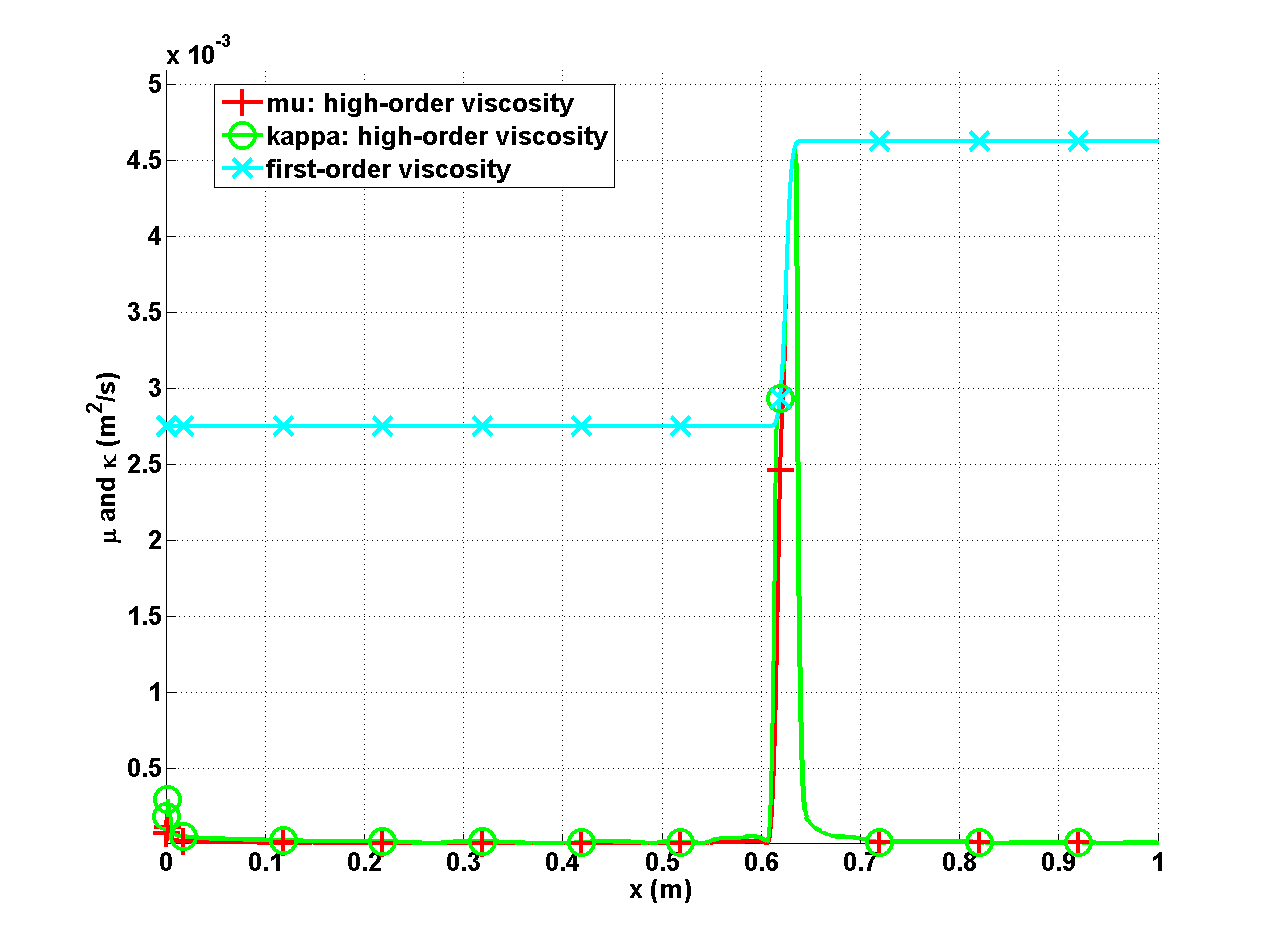
\includegraphics[width=\textwidth]{figures/SlowMovingShock_viscosity.png}
                \caption{Viscosity coefficients}
                \label{fig:viscosity_sms}
        \end{subfigure} 
        \caption{Slow moving shock profiles at $t=1.1s$.}\label{fig:low_moving_shock}
\end{figure} 

%---------------------------------------------------------------------------------------------------
\subsection{Subsonic flow over a 2-D cylinder} \label{sec:cylinder}
%---------------------------------------------------------------------------------------------------

Fluid flow over a 2-D cylinder is often used as a benchmark case to test numerical schemes in the 
low-Mach regime \cite{LowMach1, LowMach2, LowMach3}. For this test, an analytical solution is available 
in the incompressible limit and is often referred to as the potential steady-state flow solution. 
The main features of the potential flow are the following:
%
\begin{itemize}
\item The solution is symmetric: the iso-Mach contour lines are used to assess the symmetry of the numerical solution;
\item The steady-state velocity at the top of the cylinder is twice the incoming velocity set at the inlet;
\item The spatial steady-state pressure variations are proportional to the square of inlet Mach number, i.e., 
\begin{equation}
\delta P = \frac{\max(P(\vec{r})) - \min(P(\vec{r}))}{\max(P(\vec{r}))}  \propto M_\infty^2
%||\tilde{\vec{u}}|| = \frac{\max(||\vec{u}||) - \min(||\vec{u}||)}{\max(||\vec{u}||)}  \propto M_\infty\nonumber 
\end{equation}
where $\delta P$ and $M_\infty$ denote the spatial steady-state pressure variations and the inlet Mach number, respectively.
\end{itemize}
%
The computational domain consists of a $1\times 1$ square with a circular hole of radius $0.05$ in its center. 
A $\mathbb{P}_1$ triangular mesh with $4008$ triangular elements is employed to discretize the geometry. 
The ideal gas equation of state, with $\gamma=1.4$ is used. At the inlet, a subsonic stagnation boundary 
condition is used: the stagnation pressure and temperature are computed using the following relations:
%
\begin{equation}
\label{eq:stagnation_relations}
\left\{
\begin{array}{l}
P_0 = P\left( 1 + \frac{\gamma-1}{2} M^2 \right)^{\frac{\gamma-1}{\gamma}} \\
T_0 = T\left( 1 + \frac{\gamma-1}{2} M^2 \right)
\end{array}
\right.
\end{equation}
%
A static pressure boundary condition, with static pressure $P_s = 101,325$ $Pa$, is set at the outlet boundary. 
The implementation of the pressure boundary conditions is based on \cite{SEM}. A solid wall boundary condition 
is set for the top and bottom walls of the computational domain. The simulations are run until a steady state 
is reached (with a $CFL$ of $40$). When the residual norm (for all equations) is less than $10^{-12}$ the 
steady state is considered to have been reached.

Several simulations are performed, with inlet Mach numbers $M_{\text{inlet}}$ ranging from $10^{-3}$ to $10^{-7}$, 
and are shown in \fig{fig:cylinder}. The iso-Mach contour lines are drawn using 30 equally-spaced intervals, from 
$2\times 10^{-10}$ to $M_{\text{inlet}}$.
%
\begin{figure}[H]
        \centering
        \begin{subfigure}[b]{0.495\textwidth}
                \centering
                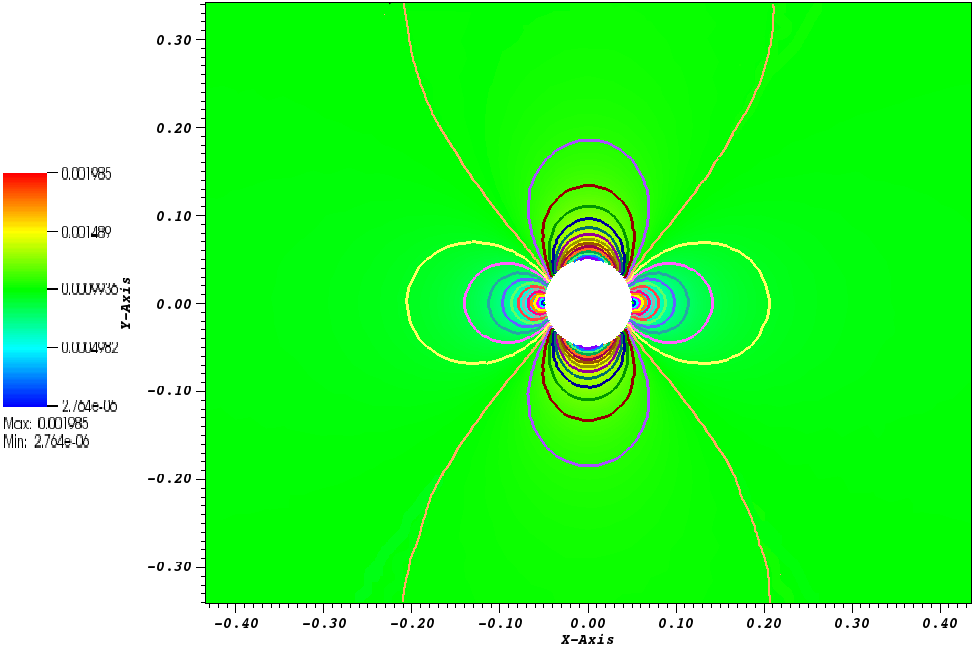
\includegraphics[width=\textwidth]{figures/CylinderMach1em3ZoomIn.png}
                \caption{$M_{\text{inlet}}=10^{-3}$}
                \label{fig:cyl_1em3}
        \end{subfigure}%
        \begin{subfigure}[b]{0.495\textwidth}
                \centering
                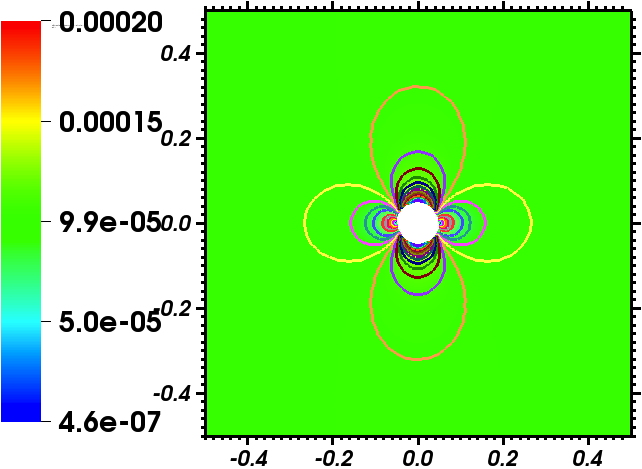
\includegraphics[width=\textwidth]{figures/CylinderMach1em4ZoomIn.png}
                \caption{$M_{\text{inlet}}=10^{-4}$}
                \label{fig:cyl_1em4}
        \end{subfigure}    

        \begin{subfigure}[b]{0.495\textwidth}
                \centering
                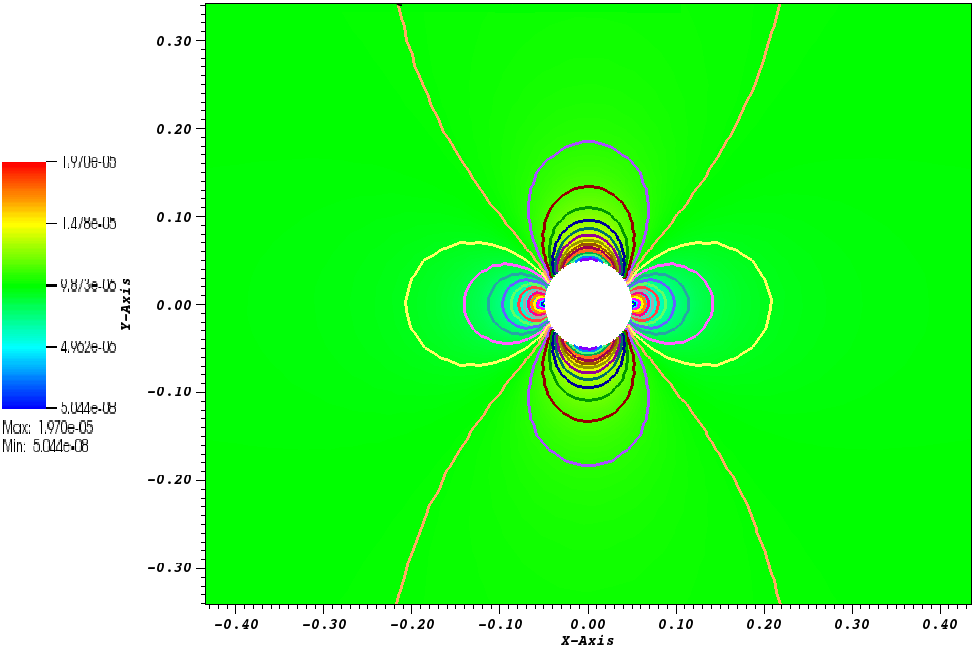
\includegraphics[width=\textwidth]{figures/CylinderMach1em5ZoomIn.png}
                \caption{$M_{\text{inlet}}=10^{-5}$}
                \label{fig:cyl_1em5}
        \end{subfigure}
        \begin{subfigure}[b]{0.495\textwidth}
                \centering
                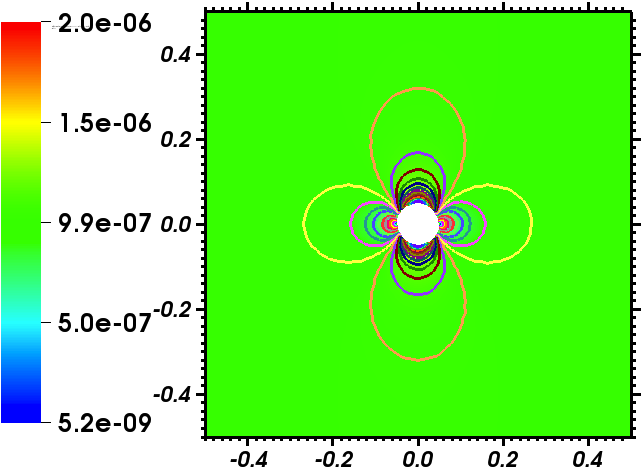
\includegraphics[width=\textwidth]{figures/CylinderMach1em6ZoomIn.png}
                \caption{$M_{\text{inlet}}=10^{-6}$}
                \label{fig:cyl_1em6}
        \end{subfigure}

        \begin{subfigure}[b]{0.495\textwidth}
                \centering
                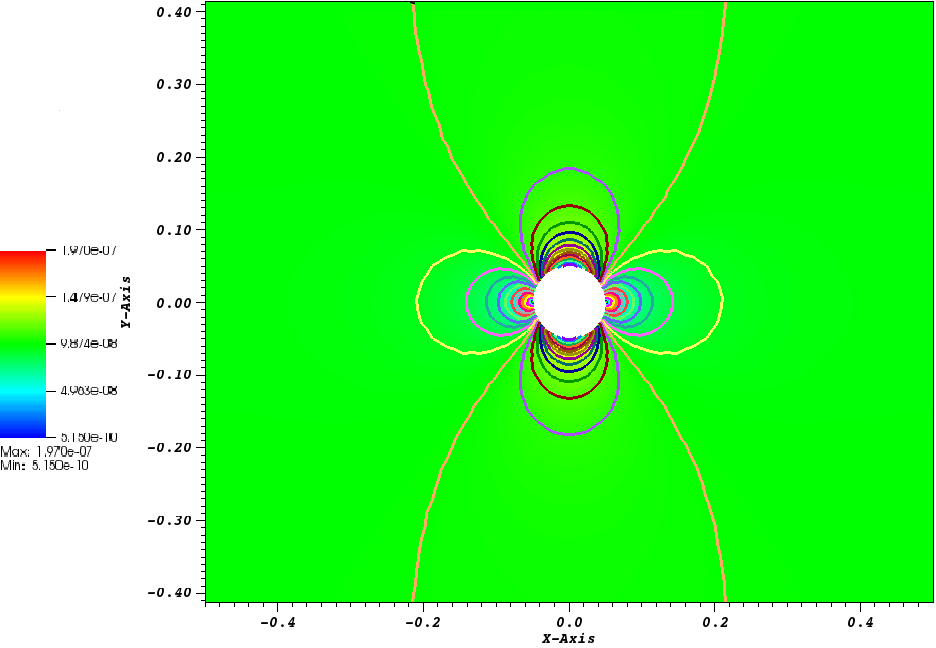
\includegraphics[width=\textwidth]{figures/CylinderMach1em7ZoomIn.png}
                \caption{$M_{\text{inlet}}=10^{-7}$}
                \label{fig:cyl_1em7}
        \end{subfigure}
        \caption{Iso-Mach lines for a subsonic flow over a 2-D cylinder with inlet Mach number values 
				from ranging from $10^{-3}$ to $10^{-7}$ (steady-state solution).}
				\label{fig:cylinder}
\end{figure}
%
The steady-state velocity at the top of the cylinder and at the inlet are given for different Mach-number values 
(ranging from $10^{-3}$ to $10^{-7}$) in \tbl{tbl:velocity_ratio}. The ratio of the inlet velocity to 
the velocity at the top of cylinder is also computed and is very close to the theoretical value of $2$ 
that is expected in the incompressible limit.
%
\begin{table}[H]
\begin{center}
 \caption{\label{tbl:velocity_ratio}Steady-state velocity ratio for different Mach numbers.}
\begin{tabular}{|c|c|c|c|}
\hline
Mach number & inlet velocity & velocity at the top of the cylinder & ratio \\ \hline
$10^{-3}$ & $2.348$ $10^{-3}$ & $1.176$ $10^{-3}$& $1.99$  \\ \hline
$10^{-4}$ & $2.285$ $10^{-4}$ & $1.145$ $10^{-4}$& $1.99$  \\ \hline
$10^{-5}$ & $2.283$ $10^{-5}$ & $1.144$ $10^{-5}$ & $1.99$ \\ \hline
$10^{-6}$ & $2.283$ $10^{-6}$ & $1.144$ $10^{-6}$ & $1.99$ \\ \hline
$10^{-7}$ & $2.283$ $10^{-7}$ & $1.144$ $10^{-7}$ & $1.99$ \\ \hline 
\end{tabular}
\end{center}
\nonumber
\end{table}
%
In \fig{fig:pressure_vel_fluc}, the spatial steady-state variations in pressure and velocity are plotted as a function of the 
Mach number (on a log-log scale). The spatial steady-state pressure variations are expected to be of the order of $M^2$ in the incompressible limit, 
which we observe. From Bernoulli's principle, this implies that the velocity spatial variations should be of order $M$ 
in the incompressible limit, which we also observe in \fig{fig:pressure_vel_fluc}. 
It is known that some stabilization methods, e.g., \cite{LowMach1, LowMach2, LowMach3}, 
can produce spatial steady-state pressure variations with the wrong Mach-number order. Here, the entropy viscosity method yields 
the correct orders in the low-Mach limit. For ease of comparison, reference lines with slope values of 1 and 2 are also plotted.
%
\begin{figure}[H]
\centering
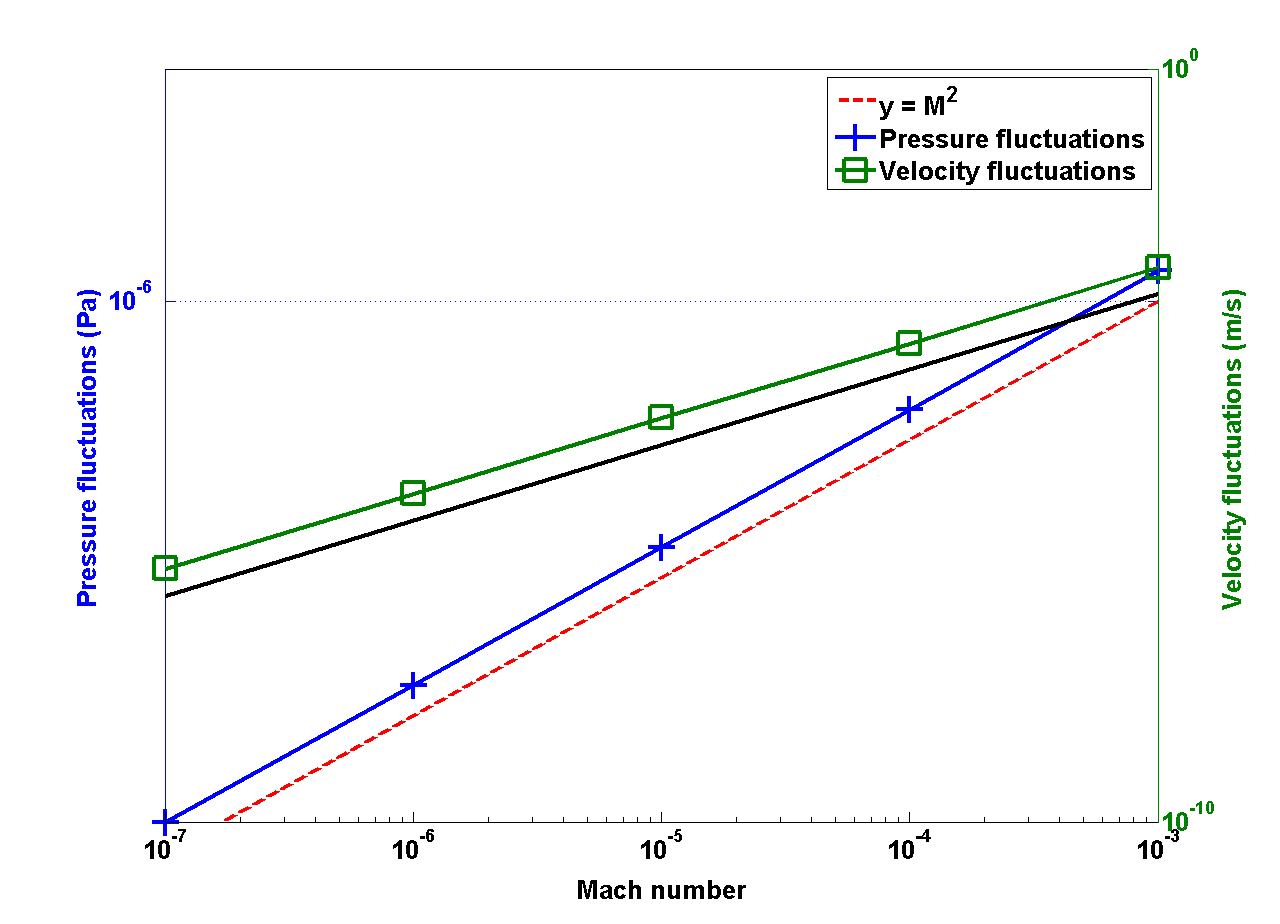
\includegraphics[width=\textwidth]{figures/pressure_fluctuation.png}
\caption{Log-log plot of the spatial steady-state pressure and velocity variations as a function of the far-field Mach number.}
\label{fig:pressure_vel_fluc}
\end{figure}

%---------------------------------------------------------------------------------------------------
\subsection{Subsonic flow over a 2-D hump} \label{sec:hump}
%---------------------------------------------------------------------------------------------------
%\tcr{Is it a circular hump or Gaussian hump in the literature???} \tcb{circular hump}

This is a another example of an internal flow configuration. It consists of a channel of height $L=1$ $m$ 
and length $3L$, with a circular bump of length $L$ and thickness $0.1L$. The bump is located on the bottom 
wall at a distance $L$ from the inlet. The system is initialized with an uniform pressure $P=101,325$ $Pa$ 
and temperature $T=300$ $K$. The initial velocity is computed from the inlet Mach number, the pressure, the 
temperature and the ideal gas equation (with  $\gamma=1.4$). Here,  $C_v = 717$ $J/kg-K$. At the inlet, a 
subsonic stagnation boundary condition is used and the stagnation pressure and temperature are computed 
using \eqt{eq:stagnation_relations}.
The static pressure $P_s = 101,325$ $Pa$ is set at the subsonic outlet. The results are shown in \fig{fig:2d_hump_mach_0p7}, 
\fig{fig:2d_hump_mach_0p01}, \fig{fig:2d_hump_mach_0p0001} and \fig{fig:2d_hump_mach_0p0000001} for the inlet 
Mach numbers $M_{\infty}=0.7$, $M_{\infty}=0.01$, $M_{\infty}=10^{-4}$ and $M_{\infty}=10^{-7}$, respectively. 
It is expected that, for low Mach numbers, the solution does not depend on the Mach number and is 
identical to the incompressible flow solution. On the other hand, for a flow with $M=0.7$, 
the compressible effects become non negligible and a shock can form. An uniform grid of $3352$ $Q_1$ elements 
was used to obtain the numerical solution for Mach numbers less than and equal to $M_{\infty}=0.01$. A spatial mesh, once refined, was 
employed for the $M_{\infty}=0.7$ simulation in order to better resolve the shock. A $CFL$ of 20 was employed 
and the simulations were run until steady state.
%
\begin{figure}[H]
        \centering
        \begin{subfigure}[b]{\textwidth}
                \centering
                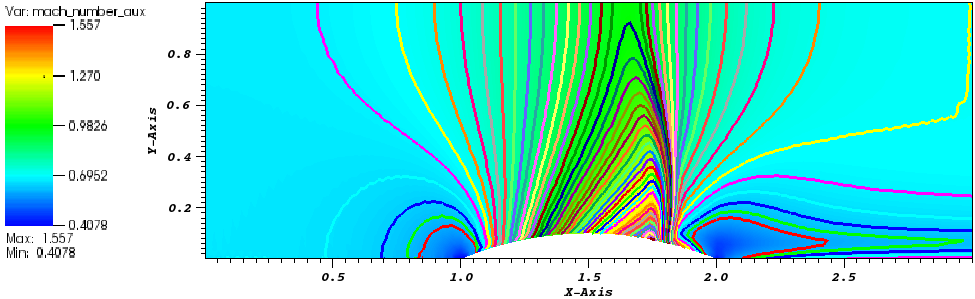
\includegraphics[width=\textwidth]{figures/Hump2D_mach_0p7.png}
                \caption{Mach $0.7$}
                \label{fig:2d_hump_mach_0p7}
        \end{subfigure}%

        \begin{subfigure}[b]{\textwidth}
                \centering
                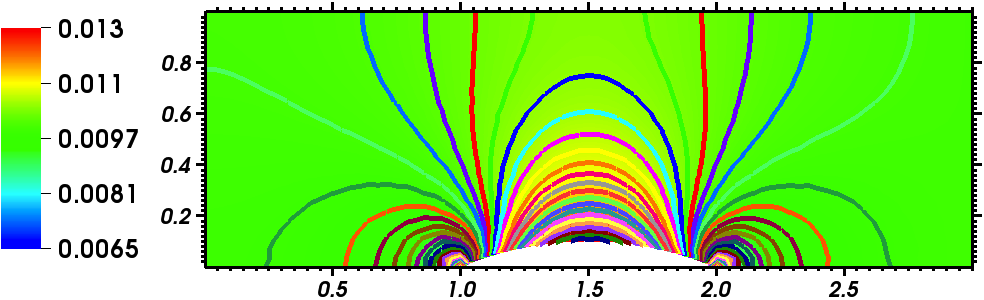
\includegraphics[width=\textwidth]{figures/Hump2D_mach_0p01.png}
                \caption{Mach $10^{-2}$}
                \label{fig:2d_hump_mach_0p01}
        \end{subfigure}%
        
        \begin{subfigure}[b]{\textwidth}
                \centering
                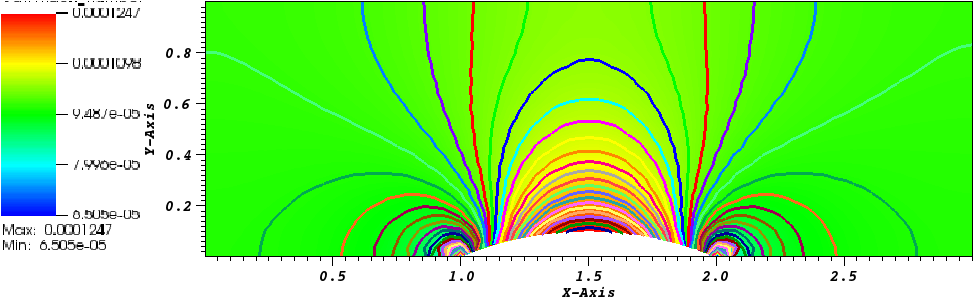
\includegraphics[width=\textwidth]{figures/Hump2D_mach_1em4.png}
                \caption{Mach $10^{-5}$}
                \label{fig:2d_hump_mach_0p0001}
        \end{subfigure}

        \begin{subfigure}[b]{\textwidth}
                \centering
                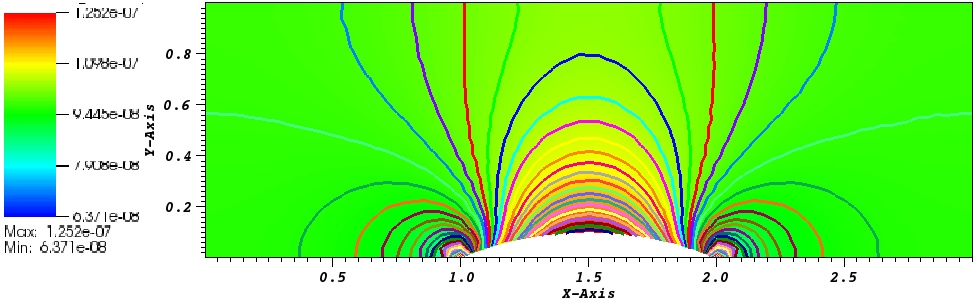
\includegraphics[width=\textwidth]{figures/Hump2D_mach_1em7.png}
                \caption{Mach $10^{-7}$}
                \label{fig:2d_hump_mach_0p0000001}
        \end{subfigure}
        \caption{Iso-Mach lines for a 2-D flow over a circular bump (steady-state solution).}
				\label{fig:2d_hump}
\end{figure}
%
The results shown in \fig{fig:2d_hump_mach_0p01}, \fig{fig:2d_hump_mach_0p0001} and \fig{fig:2d_hump_mach_0p0000001} 
correspond to the low-Mach regime. The iso-Mach lines are drawn ranging from the minimum and the maximum values 
(provided in each legend) using 50 equally-spaced intervals. The steady-state solution is symmetric and does not 
depend on the value of the inlet Mach number, as expected in the incompressible limit. 

In \fig{fig:2d_hump_mach_0p7}, the steady-state numerical solution develops a shock: the compressibility effects 
are no longer small. The iso-Mach lines are also plotted with 50 intervals and range from $0.4$ to $1.6$. 
The shock is well resolved and does not display any instabilities or spurious oscillations. 

%---------------------------------------------------------------------------------------------------
\subsection{Supersonic flow in a compression corner} \label{sec:corner}
%---------------------------------------------------------------------------------------------------

In this last example, we consider a supersonic flow at Mach 2.5 impinging on a corner with an angle of $15^\circ$. 
From the oblique shock theory \cite{CompressionCorner}, an analytical solution for this supersonic flow is available 
and gives the downstream-to-upstream pressure, entropy and Mach number ratios. 
The initial conditions are chosen to be spatially uniform: the pressure and temperature are set to $P=101,325$ $Pa$ 
and $T=300$ $K$, respectively.  The ideal gas equation of state is used with the same parameters as in \sct{sec:hump}. 
The initial velocity is computed from the upstream Mach number. The inlet is supersonic and therefore, the pressure, 
temperature and velocity are specified using Dirichlet boundary conditions. The outlet is also supersonic and none 
of the characteristics enter the domain through this boundary; the values are computed by the solver.

The simulation is run with $CFL=2$ until steady state is reached. A 2-D mesh made of $16,109$ $\mathbb{Q}_1$ elements 
is used. The ratios for pressure, entropy and Mach number computed using the analytical (published with only two 
significant digits) and the numerical solutions are given in \tbl{tbl:corner_exact_sol}; they are in excellent 
agreement. The shock wave angle at steady state is also known and given by the so-called $\theta -\beta -M$ relation:
%
\begin{equation}
\tan \theta = 2 \cot \beta \frac{M^2 \sin^2 \beta -1}{M^2 \left(\gamma+\cos^2 (2\beta)\right)+2} ,
\end{equation}
%
where $\theta$, $\beta$ and $M$ denote the corner angle, the shock wave angle, and the upstream Mach number, respectively. 
For Mach 2.5 and a 15$^\circ$ corner angle, the analytical value for the shock wave angle is $36.94^\circ$ 
at steady state. From \fig{fig:2d_corner_mach}, the numerical value of the shock wave angle can be measured 
and is found to be equal to $36.9^{\circ}$ and thus is in excellent agreement with the theory.
%
\begin{table}[H]
\begin{center}
\begin{tabular}{|c|c|c|}  \hline
            & analytical & numerical\\ \hline
Pressure    & 2.47       & 2.467    \\ \hline
Mach number &  0.74      & 0.741    \\ \hline
Entropy     & 1.03       & 1.026    \\ \hline 
\end{tabular}
\caption{\label{tbl:corner_exact_sol} Ratio of analytical and numerical downstream to upstream quantities for 
the compression corner problems (corner angle of $15^\circ$ and inlet $M=2.5$ (analytical values from \cite{CompressionCorner}).}
\end{center}
\end{table}
%
\begin{figure}[H]
        \centering
        \begin{subfigure}[b]{0.52\textwidth}
                \centering
                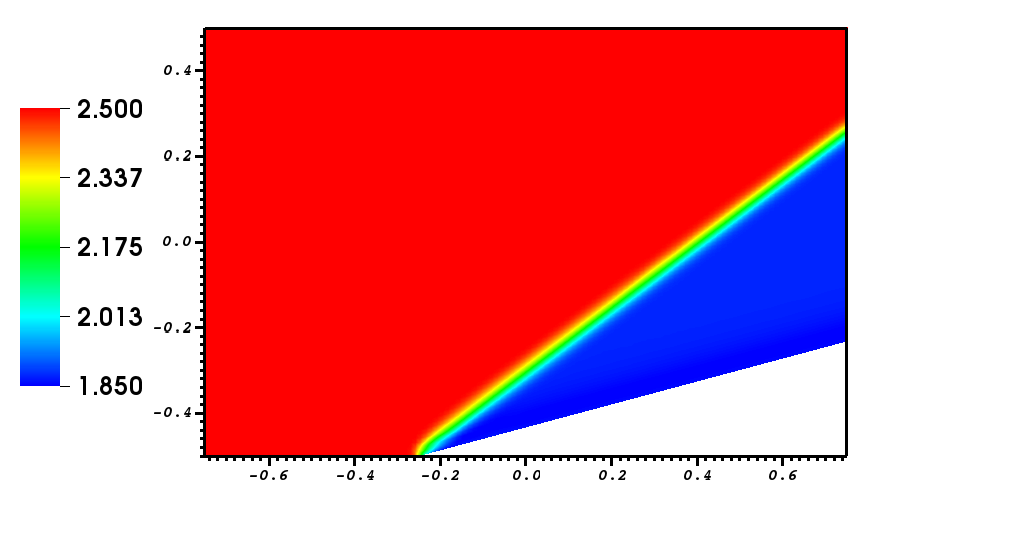
\includegraphics[width=\textwidth]{figures/CompressionCorner2D_mach.png}
                \caption{Mach number}
                \label{fig:2d_corner_mach}
        \end{subfigure}%
        \begin{subfigure}[b]{0.52\textwidth}
                \centering
                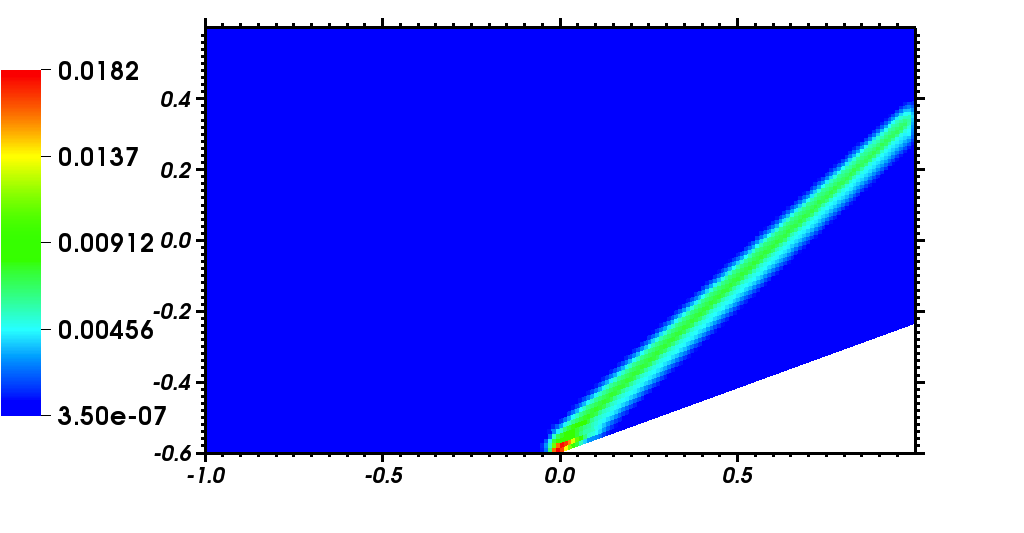
\includegraphics[width=\textwidth]{figures/CompressionCorner2D_viscosity.png}
                \caption{Viscosity coefficients}
                \label{fig:2d_corner_visc}
        \end{subfigure}
        
        \begin{subfigure}[b]{0.49\textwidth}
                \centering
                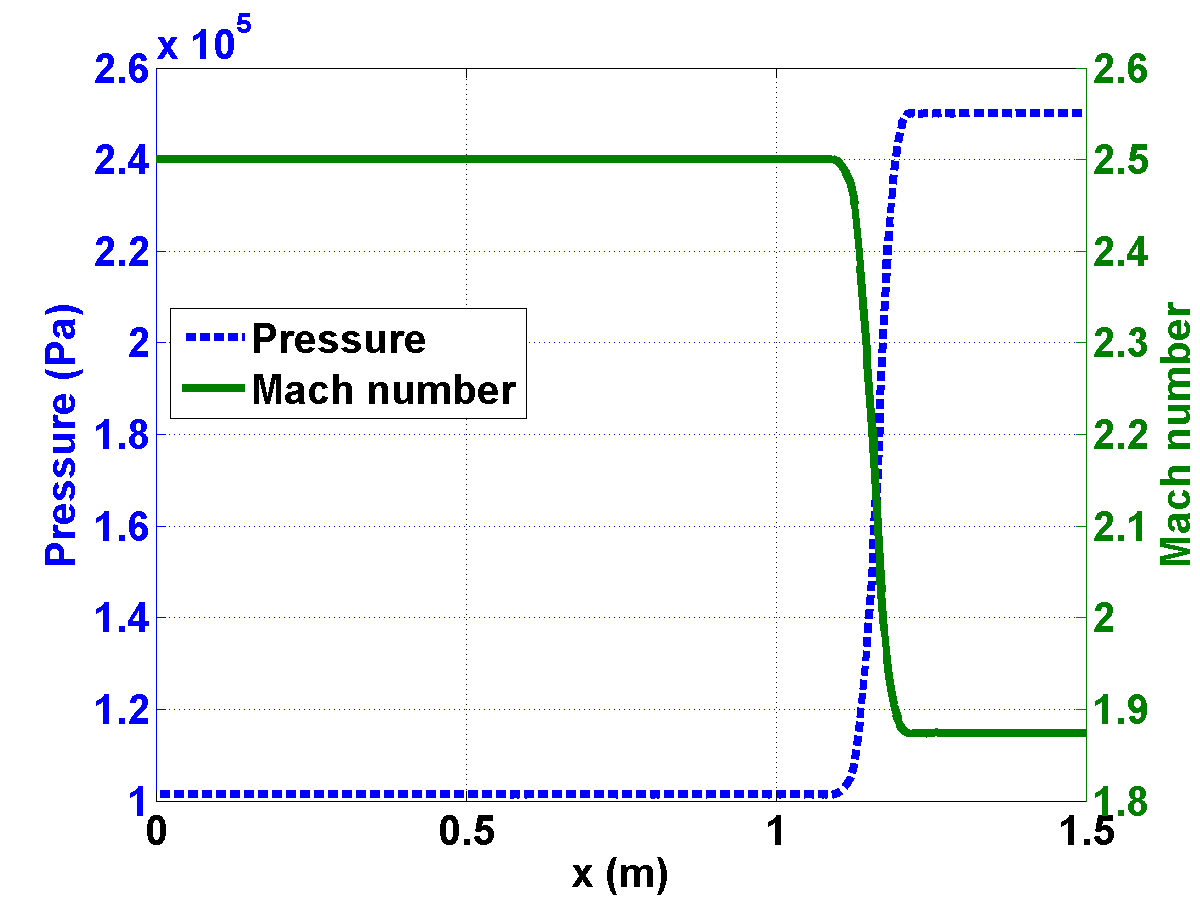
\includegraphics[width=\textwidth]{figures/mach_number_pressure.png}
                \caption{Pressure and Mach number}
                \label{fig:2d_corner_isomach}
        \end{subfigure}        
        \begin{subfigure}[b]{0.49\textwidth}
                \centering
                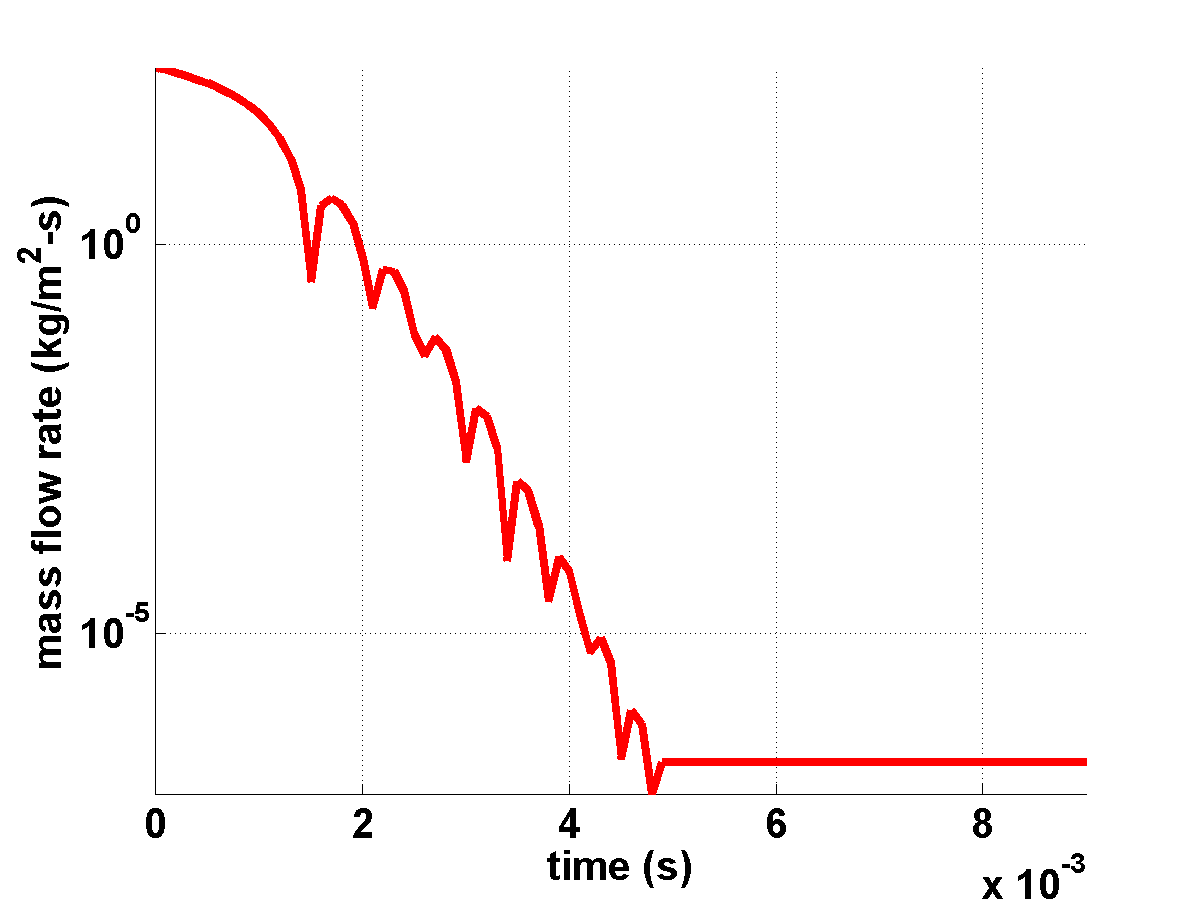
\includegraphics[width=\textwidth]{figures/CompressionCorner2DQ.png}
                \caption{Difference between inlet and outlet mass flow rates as a function of time.}
                \label{fig:2d_convergence}
        \end{subfigure}
        \caption{Steady-state solution for a flow in a 2-D compression corner.}\label{fig:2d_corner}
\end{figure}
%
The steady-state numerical solution is given in \fig{fig:2d_corner}; the Mach number and the viscosity 
coefficients are plotted in \fig{fig:2d_corner_mach} and \fig{fig:2d_corner_visc}, respectively. The 
steady-state solution is composed of two regions of constant state separated by an oblique shock. 
\fig{fig:2d_corner_visc} shows that the viscosity coefficient is large in the shock and small elsewhere, 
as expected. At the location of the corner ($x=-0.25m$, $y=-0.5m$), the viscosity coefficient is peaked 
because of the treatment of the wall boundary condition: at this particular node, the normal is not well 
defined and may cause some numerical errors. The 1-D graphs at $y=0$ for the pressure and the Mach number 
are given in \fig{fig:2d_corner_isomach}: no spurious oscillations are observed and the shock is well resolved. 
Finally, the difference between the inlet and outlet mass flow rates is plotted in \fig{fig:2d_convergence} 
and shows that a steady state has indeed been reached. 

The results presented in this paper demonstrate the ability of the entropy viscosity method with the new definitions of the viscosity coefficients 
to correctly simulate several types of flows (from very low Mach subsonic to transonic flows) without tuning parameters.


%%%%%%%%%%%%%%%%%%%%%%%%%%%%%%%%%%%%%%%%%%%%%%%%%%%%%%%%%%%%%%%%%%%%%%%%%%%%%%%%%%%%%%%%%%%%%%%%%%%%
%%%%%%%%%%%%%%%%%%%%%%%%%%%%%%%%%%%%%%%%%%%%%%%%%%%%%%%%%%%%%%%%%%%%%%%%%%%%%%%%%%%%%%%%%%%%%%%%%%%%
\section{Conclusions} \label{sec:ccl}
%%%%%%%%%%%%%%%%%%%%%%%%%%%%%%%%%%%%%%%%%%%%%%%%%%%%%%%%%%%%%%%%%%%%%%%%%%%%%%%%%%%%%%%%%%%%%%%%%%%%
%%%%%%%%%%%%%%%%%%%%%%%%%%%%%%%%%%%%%%%%%%%%%%%%%%%%%%%%%%%%%%%%%%%%%%%%%%%%%%%%%%%%%%%%%%%%%%%%%%%%

A new version of the entropy viscosity method that is valid for a wide range of Mach numbers has been derived 
and presented for the inviscid Euler equations.
The definition of the viscosity coefficients
is now consistent with the low-Mach asymptotic limit, does not require an analytical expression 
for the entropy function, and is therefore applicable to a larger variety of flow regimes, from very 
low-Mach flows to supersonic flows. 
The method has also been extended to Euler equation with variable area to solve nozzle flow problems.
In 1-D, convergence of the numerical solution to 
the exact solution was demonstrated by computing the convergence rates of the L$1$ and L$2$ norms 
for flows in a converging-diverging nozzle and in straight pipes. For smooth solutions, second-order 
convergence was verified; solutions with shocks converged with the expected theoretical rates of 1 (L$_1$-norm)
and 0.5 (L$_2$-norm).

The effectiveness of the method was also demonstrated in 2-D using a series of benchmark problems
for both subsonic and supersonic flows in various geometries, with Mach numbers ranging from $10^{-7}$ to 
2.5. For very low-Mach flows, we numerically verified that the spatial steady-state pressure variations were proportional to 
the square of the Mach number, as expected in the incompressible limit.

In the future, we plan to further extend the entropy viscosity method to the seven-equation two-phase flow fluid model \cite{SEM}. 
This two-phase flow system of equations is a good candidate for two reasons: it is unconditionally hyperbolic and degenerates to the standard Euler equations when one phase disappears.

%%%%%%%%%%%%%%%%%%%%%%%%%%%%%%%%%%%%%%%%%%%%%%%%%%%%%%%%%%%%%%%%%%%%%%%%%%%%%%%%%%%%%%%%%%%%%%%%%%%%
%%%%%%%%%%%%%%%%%%%%%%%%%%%%%%%%%%%%%%%%%%%%%%%%%%%%%%%%%%%%%%%%%%%%%%%%%%%%%%%%%%%%%%%%%%%%%%%%%%%%

%%%%%%%%%%%%%%%%%%%%%%%%%%%%%%%%%%%%%%%%%%%%%%%%%%%%%%%%%%%%%%%%%%%%%%%%%%%%%%%%%%%%%%%%%%%%%%%%%%%%
%%%%%%%%%%%%%%%%%%%%%%%%%%%%%%%%%%%%%%%%%%%%%%%%%%%%%%%%%%%%%%%%%%%%%%%%%%%%%%%%%%%%%%%%%%%%%%%%%%%%
\section*{Acknowledgments} 
The authors (M.D. and J.R.) would like to thank Bojan Popov and Jean-Luc Guermond for many fruitful discussions.  
The research was carried out under the auspices the Idaho National Laboratory for the US Department of Energy.

%%%%%%%%%%%%%%%%%%%%%%%%%%%%%%%%%%%%%%%%%%%%%%%%%%%%%%%%%%%%%%%%%%%%%%%%%%%%%%%%%%%%%%%%%%%%%%%%%%%%
%%%%%%%%%%%%%%%%%%%%%%%%%%%%%%%%%%%%%%%%%%%%%%%%%%%%%%%%%%%%%%%%%%%%%%%%%%%%%%%%%%%%%%%%%%%%%%%%%%%%
\bibliography{mybibfile}
%%%%%%%%%%%%%%%%%%%%%%%%%%%%%%%%%%%%%%%%%%%%%%%%%%%%%%%%%%%%%%%%%%%%%%%%%%%%%%%%%%%%%%%%%%%%%%%%%%%%
%%%%%%%%%%%%%%%%%%%%%%%%%%%%%%%%%%%%%%%%%%%%%%%%%%%%%%%%%%%%%%%%%%%%%%%%%%%%%%%%%%%%%%%%%%%%%%%%%%%%
\newpage
%%%%%%%%%%%%%%%%%%%%%%%%%%%%%%%%%%%%%%%%%%%%%%%%%%%%%%%%%%%%%%%%%%%%%%%%%%%%%%%%%%%%%%%%%%%%%%%%%%%%
%%%%%%%%%%%%%%%%%%%%%%%%%%%%%%%%%%%%%%%%%%%%%%%%%%%%%%%%%%%%%%%%%%%%%%%%%%%%%%%%%%%%%%%%%%%%%%%%%%%%
\appendix
%%%%%%%%%%%%%%%%%%%%%%%%%%%%%%%%%%%%%%%%%%%%%%%%%%%%%%%%%%%%%%%%%%%%%%%%%%%%%%%%%%%%%%%%%%%%%%%%%%%%
%%%%%%%%%%%%%%%%%%%%%%%%%%%%%%%%%%%%%%%%%%%%%%%%%%%%%%%%%%%%%%%%%%%%%%%%%%%%%%%%%%%%%%%%%%%%%%%%%%%%

%%%%%%%%%%%%%%%%%%%%%%%%%%%%%%%%%%%%%%%%%%%%%%%%%%%%%%%%%%%%%%%%%%%%%%%%%%%%%%%%%%%%%%%%%%%%%%%%%%%%
%%%%%%%%%%%%%%%%%%%%%%%%%%%%%%%%%%%%%%%%%%%%%%%%%%%%%%%%%%%%%%%%%%%%%%%%%%%%%%%%%%%%%%%%%%%%%%%%%%%%
\section{Derivation of the entropy residual as a function of density, pressure, and speed of sound} \label{app:ent_res}
%%%%%%%%%%%%%%%%%%%%%%%%%%%%%%%%%%%%%%%%%%%%%%%%%%%%%%%%%%%%%%%%%%%%%%%%%%%%%%%%%%%%%%%%%%%%%%%%%%%%
%%%%%%%%%%%%%%%%%%%%%%%%%%%%%%%%%%%%%%%%%%%%%%%%%%%%%%%%%%%%%%%%%%%%%%%%%%%%%%%%%%%%%%%%%%%%%%%%%%%%

The entropy residual is defined as follows:
%
\begin{equation*}
\resi(\vec{r},t) = \partial_t s (\vec{r},t) + \vec{u} \cdot \grad s (\vec{r},t) ,
\end{equation*}
%
where all variables were defined previously. This form of the entropy residual is not suitable for the low-Mach 
limit as explained in \sct{sec:background}. In this appendix, we recast the entropy residual $\resi(\vec{r},t)$ 
as a function of the primitive variables (pressure, velocity and density) and the speed of sound. The first step 
of this derivation is to use the chain rule, recalling that the entropy is a function of the internal energy $e$ 
and the density $\rho$, yielding
%
\begin{equation*}
\resi(\vec{r},t) = s_e  \matder{e} + s_{\rho}  \matder{\rho} \,,.
\end{equation*}
%
where $s_e$ denotes the partial derivative of $s$ with respect to the variable $e$. We recall that $\matder{\ }$ 
denotes the material derivative. Since the internal energy $e$ is a function of pressure $P$ and density $\rho$ 
(through the equation of state), we use again the chain rule to re-express the previous equation as a function 
of the material derivatives in $P$ and $\rho$:
%
\begin{eqnarray*}
\resi(\vec{r},t) &=&  s_e e_P \matder{P} + ( s_e e_{\rho} + s_{\rho} ) \matder{\rho} \\
&=& s_e e_P \left( \matder{P} + \frac{1}{s_e e_P} ( s_e e_{\rho} + s_{\rho} )  \matder{\rho}\right) \\
&=& s_e e_P \left( \matder{P} + ( \frac{e_{\rho}}{e_P} + \frac{s_{\rho}}{s_e e_P} )  \matder{\rho} \right) \,.
\end{eqnarray*}
%
To prove that the term multiplying the material derivative of the density is indeed equal to the square of the speed 
of sound, we recall that the speed of sound is defined as the partial derivative of pressure with respect to density 
at constant entropy, which can be recast as a function of the entropy as follows (see Appendix A.2 of \cite{jlg}):
%
\begin{equation*}
c^2 := \left. \frac{\partial P}{\partial \rho} \right|_{s=cst} = P_{\rho} - \frac{s_{\rho}}{s_e} P_e   \, .
\end{equation*}
%
Using the following relations (see Appendix A.1 of \cite{jlg})
%
\begin{equation*}
P_e = \frac{1}{e_P} \text{ and } P_{\rho} = -\frac{e_{\rho}}{e_P}  \, .
\end{equation*}
%
Substitution of these expressions into the entropy residual equation above gives \eqt{eq:ent_res}, which is recalled 
below for completeness:
%
\begin{equation*}
\resi(\vec{r},t) := \partial_t s + \vec{u} \cdot \grad s = \matder{s} = \frac{s_e}{P_e} \left( \underbrace{\matder{P} - c^2 \matder{\rho} }_{\resinew(\vec{r},t)} \right) \, .
\end{equation*} 

%%%%%%%%%%%%%%%%%%%%%%%%%%%%%%%%%%%%%%%%%%%%%%%%%%%%%%%%%%%%%%%%%%%%%%%%%%%%%%%%%%
\newpage
%%%%%%%%%%%%%%%%%%%%%%%%%%%%%%%%%%%%%%%%%%%%%%%%%%%%%%%%%%%%%%%%%%%%%%%%%%%%%%%%%%%%%%%%%%%%%%%%%%%%
%%%%%%%%%%%%%%%%%%%%%%%%%%%%%%%%%%%%%%%%%%%%%%%%%%%%%%%%%%%%%%%%%%%%%%%%%%%%%%%%%%%%%%%%%%%%%%%%%%%%
\section{Derivation of the dissipative terms for the Euler equations with variable area using the entropy minimum principle} \label{app:diss_terms}
%%%%%%%%%%%%%%%%%%%%%%%%%%%%%%%%%%%%%%%%%%%%%%%%%%%%%%%%%%%%%%%%%%%%%%%%%%%%%%%%%%%%%%%%%%%%%%%%%%%%
%%%%%%%%%%%%%%%%%%%%%%%%%%%%%%%%%%%%%%%%%%%%%%%%%%%%%%%%%%%%%%%%%%%%%%%%%%%%%%%%%%%%%%%%%%%%%%%%%%%%
%
The Euler equations (without viscous regularization) with variable area are recalled here
%
\begin{subequations}
\label{app:euler_variable_A}
%
\begin{equation}
\partial_t \left( \rho A \right) + \div \left( \rho \vec{u} A \right) = 0 
\end{equation}
%
\begin{equation}
\partial_t \left( \rho \vec{u} A \right) + \div \left[A\left( \rho \vec{u} \otimes \vec{u} + P \mathbb{I} \right) \right] = P \grad A 
\end{equation}
% 
\begin{equation}
\partial_t \left( \rho E A \right) + \div \left[ \vec{u} A \left( \rho E + P \right) \right] = 0 \,.
\end{equation}
\end{subequations}
%
The specific entropy is a function of the density $\rho$ and the internal energy $e$, i.e., $s(e,\rho)$. The 
above system of equations satisfies the minimum entropy principle \cite{Leveque},
%
\begin{equation}
A \rho \left( \partial_t s + \vec{u} \cdot \div s \right) \geq 0 \, .
\end{equation}
%
The entropy function $s$ satisfies the second law of thermodynamics, $T ds = de - \frac{P}{\rho^2} d \rho$, 
which implies $s_e := T^{-1}$ and $s_\rho := -P T^{-1} \rho^{-2}$. One can show that \cite{jlg}
%
\begin{equation}
s_e = T^{-1} \geq 0 \text{ and }
Ps_e + \rho^2 s_{\rho} = 0 \,.
\end{equation}
%
In order to apply the entropy viscosity method to the variable-area Euler equations, dissipative terms need to 
be added to each equation in \eqt{app:euler_variable_A}. The functional forms of these terms need to be such 
that the entropy residual derived with these terms present also satisfies the minimum entropy principle. 
To prove the minimum entropy principle, the extra terms appearing in the entropy residual are either recast as 
conservative terms or shown to be positive. The rest of this appendix presents this demonstration. 
Following \cite{jlg}, we first write the variable-area equations with dissipative terms: 
%
%
\begin{subequations}
\label{app:euler_variable_A_diss}
%
\begin{equation}
\partial_t \left( \rho A \right) + \div \left( \rho \vec{u} A \right) = \div f 
\end{equation}
%
\begin{equation}
\partial_t \left( \rho \vec{u} A \right) + \div \left[A\left( \rho \vec{u} \otimes \vec{u} + P \mathbb{I} \right) \right] = P \grad A + \div g
\end{equation}
% 
\begin{equation}
\partial_t \left( \rho E A \right) + \div \left[ \vec{u} A \left( \rho E + P \right) \right] = \div ( h + \vec{u} \cdot g )  \,.
\end{equation}
\end{subequations}
%
where $f$, $g$ and $h$ are dissipative fluxes to be determined. Starting from the modified system of equations 
given in \eqt{app:euler_variable_A_diss}, the entropy residual is derived again. The derivation requires the 
following steps : express the governing laws in terms of primitive variables $(\rho, \vec{u}, e)$, multiply the 
continuity equation by $\rho s_\rho$ and the internal energy equation by $s_e$, and invoke multivariate chain 
rule, e.g., $\partial s /\partial x = s_e \partial e /\partial x + s_\rho \partial \rho /\partial x$. These steps 
are similar to those used for the standard Euler equations \cite{jlg}. Some of the lengthy algebra is omitted here. The above steps yield:
%
\begin{equation}
\label{eq:ent_res_app}
A \rho \left( \partial_t s + \vec{u} \cdot \grad s \right) = s_e \left[ \div h + g : \grad u + \left( \frac{u^2}{2}-e \right) \div f \right] 
+ \rho s_{\rho} \div f \,. 
\end{equation}
%
The next step consists of choosing a definition for each of the dissipative terms so that the left hand-side is positive. 
The right hand-side of \eqt{eq:ent_res_app} can be simplified using the relations $g = A \mu \grad^s \vec{u} + f \otimes \vec{u}$ and $h = \tilde{h} - 0.5 || \vec{u} ||^2 f$ to give
%
\begin{equation}
\label{eq:ent_res_app2}
A \rho \left( \partial_t s + \vec{u} \cdot \div s \right) = s_e \left[ \div \tilde{h}-e \div f \right] + \rho s_{\rho} \div f  + A s_e \mu \grad \vec{u}^s : \grad \vec{u} \,. 
\end{equation}
%
The right hand-side is now integrated by parts:
%
\begin{multline}
\label{eq:ent_res_app3}
A \rho \left( \partial_t s + \vec{u} \cdot \div s \right) = \div \left[ s_e \tilde{h}-s_e e f  + \rho s_{\rho} f \right]  \\
-\div \tilde{h} \grad s_e  + f \cdot \grad (e s_e) -  f \cdot \grad ( \rho s_{\rho} ) + A s_e \mu \grad^s \vec{u} : \grad \vec{u} 
\end{multline}
%
where $\grad^s$ is the symmetric gradient. The term $A s_e \mu \grad^s \vec{u} : \grad \vec{u}$ is positive and thus, 
does not need any further modification. It %
remains to treat the other terms of the right hand-side that we now call $rhs$:
%
\begin{equation}
rhs = \div \left[ s_e \tilde{h}-s_e e f  + \rho s_{\rho} f \right] - \tilde{h} \cdot \grad s_e  + f \cdot \grad (e s_e) - f \cdot \grad ( \rho s_{\rho} )  \,. \nonumber
\end{equation}
%
The first term in $rhs$ is a conservative term. By carefully choosing a definition for $\tilde{h}$ and $f$, the 
conservative term can be expressed as a function of the entropy $s$. The inclusion of the variable area in the 
choice of the dissipative terms is also required so that, when assuming constant area, the standard Euler 
equations are recovered. The following definitions for $\tilde{h}$ and $f$ are chosen:
%
\begin{equation}
\tilde{h} = A \kappa \grad ( \rho e ) \text{  and  } f = A \kappa \grad \rho, \nonumber 
\end{equation}
%
which yields, using the chain rule,
%
\begin{equation}
rhs = \div (\rho A \kappa \grad s ) - A \kappa \underbrace{\left[ \grad (\rho e) \grad s_e  - \grad \rho \grad (e s_e) +  \grad \rho \grad ( \rho s_{\rho} )  \right]}_{\mathbf{Q}} \nonumber
\end{equation}
%
It remains to treat the term $\mathbf{Q}$ that can be recast under a quadratic form. Following \cite{jlg}, one obtain:
%
\begin{eqnarray}
\mathbf{Q} &=& \rho X^t \Sigma X \nonumber \\
\text{with } X &=& \begin{bmatrix}
\grad \rho \\
\grad e 
\end{bmatrix}
\text{and } \Sigma = \begin{bmatrix}
       \rho^{-2}\partial_{\rho} (\rho^2 \partial_{\rho} s) & \partial_{\rho,e} s  \\[0.3em]
       \partial_{\rho,e} s & \partial_{e,e} s           \\[0.3em]
     \end{bmatrix} \nonumber 
\end{eqnarray}
%
The matrix $\Sigma$ is symmetric and identical to the matrix obtained in \cite{jlg}. The sign of the quadratic form 
can be simply determined by studying the positiveness of the matrix $\Sigma$. In this particular case, it is required 
to prove that the matrix is negative definite: the quadratic form is on the right hand-side and is preceded by a negative 
sign. According to \cite{jlg}, the convexity of the opposite of the entropy function, i..e, $-s$, with respect to the internal energy $e$ 
and the specific volume $1/ \rho$ is sufficient to ensure that the matrix $\Sigma$ is negative definite. \\
Thus, the right hand-side of the entropy residual \eqt{eq:ent_res_app} is now either recast as conservative terms, 
or known to be positive. Thus, the entropy minimum principle holds.

%%%%%%%%%%%%%%%%%%%%%%%%%%%%%%%%%%%%%%%%%%%%%%%%%%%%%%%%%%%%%%%%%%%%%%%%%%%%%%%%%%
\newpage
%%%%%%%%%%%%%%%%%%%%%%%%%%%%%%%%%%%%%%%%%%%%%%%%%%%%%%%%%%%%%%%%%%%%%%%%%%%%%%%%%%%%%%%%%%%%%%%%%%%%
%%%%%%%%%%%%%%%%%%%%%%%%%%%%%%%%%%%%%%%%%%%%%%%%%%%%%%%%%%%%%%%%%%%%%%%%%%%%%%%%%%%%%%%%%%%%%%%%%%%%
\section{Entropy residual for isentropic flows} \label{app:ise_equ}
%%%%%%%%%%%%%%%%%%%%%%%%%%%%%%%%%%%%%%%%%%%%%%%%%%%%%%%%%%%%%%%%%%%%%%%%%%%%%%%%%%%%%%%%%%%%%%%%%%%%
%%%%%%%%%%%%%%%%%%%%%%%%%%%%%%%%%%%%%%%%%%%%%%%%%%%%%%%%%%%%%%%%%%%%%%%%%%%%%%%%%%%%%%%%%%%%%%%%%%%%
\tcr{I cannot find a reference to this appendix in the main body of the manuscript. Add one.\\}
This appendix shows that the entropy residual is zero for isentropic flows. For convenience, we recall
here the entropy residual as a function of the pressure, density, velocity, and speed of sound:
%
\begin{equation}\label{eq:app_entr}
\resinew = \matder P - c^2  \matder \rho \,.
\end{equation}
%
Assuming an isentropic flow, pressure is only a function of density, i.e., $P = f( \rho )$ or equivalently $\rho = f^{-1}( P )$. 
Using the definition of the speed of sound $c^2 = \left. \frac{\partial P}{\partial \rho} \right)_s$ and the above 
form of the equation of state, we have
%
\begin{equation}\label{eq:app_sp}
c^2 = \left. \frac{\partial P}{\partial \rho} \right)_s = \frac{d P}{d \rho} = \frac{d f(\rho)}{d \rho} \,.
\end{equation}
%
Using the chain rule, the entropy residual in \eqt{eq:app_entr} can be recast as follows and proven equal to zero:
%
\begin{equation}
\resinew = \frac{d f(\rho)}{d \rho}  \matder \rho - c^2  \matder  \rho  
         = c^2                       \matder \rho - c^2  \matder  \rho  
         =  0 \,.
\end{equation}

%%%%%%%%%%%%%%%%%%%%%%%%%%%%%%%%%%%%%%%%%%%%%%%%%%%%%%%%%%%%%%%%%%%%%%%%%%%%%%%%%%%%%%%%%%%%%%%%%%%%
%%%%%%%%%%%%%%%%%%%%%%%%%%%%%%%%%%%%%%%%%%%%%%%%%%%%%%%%%%%%%%%%%%%%%%%%%%%%%%%%%%%%%%%%%%%%%%%%%%%%
\end{document}
%%%%%%%%%%%%%%%%%%%%%%%%%%%%%%%%%%%%%%%%%%%%%%%%%%%%%%%%%%%%%%%%%%%%%%%%%%%%%%%%%%%%%%%%%%%%%%%%%%%%
%%%%%%%%%%%%%%%%%%%%%%%%%%%%%%%%%%%%%%%%%%%%%%%%%%%%%%%%%%%%%%%%%%%%%%%%%%%%%%%%%%%%%%%%%%%%%%%%%%%%
